% REMEMBER: You must not plagiarise anything in your report. Be extremely careful.

\documentclass{l4proj}

    
\usepackage{adjustbox}
\usepackage{natbib}
\usepackage{subcaption}
\usepackage{float}
\usepackage{booktabs}
\usepackage{graphicx}
\usepackage[table]{xcolor} 
\usepackage{colortbl} 
\usepackage{hhline} 
\usepackage{array}
\usepackage{listings}




% Define colors
\definecolor{HeaderColor}{rgb}{0.6, 0.8, 1}
\definecolor{RowColor}{rgb}{0.9, 0.9, 0.9}

\begin{document}

%==============================================================================
%% METADATA
\title{GlasgowSupportBot: A Chatbot Companion for Academic and Wellbeing Support}
\author{Mohammed Nader Al Haffar}
\date{March 3, 2024}

\maketitle

%==============================================================================
%% ABSTRACT
\begin{abstract}
The University of Glasgow supports its students by providing a range of academic and well-being services. These include disability, good cause, and international support services. Despite the valuable resources available, navigating them can be challenging for new students. Students might be unaware of the existence of certain services or struggle to locate the information they need. GlasgowSupportBot offers a chatbot interface that serves as a guide to the University's support services. Functioning as a centralized source of information, GlasgowSupportBot is equipped with comprehensive data on various services. This interface aims to direct users to the specific support they need, mirroring the functionality of ChatGPT but customized within the University context. After conducting user evaluation, the web app received an "excellent" rating in usability. This was determined by computing the System Usability Scale (SUS) score from 23 participants, resulting in an average score of 88.5 out of 100. GlasgowSupportBot is a valuable tool for empowering students to access and utilize the University's support services efficiently.
\end{abstract}


%==============================================================================
%% ACKNOWLEDGE
\chapter*{Acknowledgements}
I am deeply grateful to Dr. Mireilla Bikanga Ada for her guidance and support throughout my dissertation journey. Over the past year, her expertise and insights have significantly shaped this work. This dissertation would not have been possible without her help. Her significant contribution to my academic journey has been invaluable, and I am thankful for the opportunity to have learned and grown under her mentorship.
Additionally, I would like to express my gratitude to my friends and family. Their consistent support and encouragement throughout my undergraduate degree have been significant.

% EDUCATION REUSE CONSENT FORM

%
\def\consentname {Mohammed Nader Al Haffar} % your full name
\def\consentdate {3 March 2023} % the date you agree
%
\educationalconsent


%==============================================================================
\tableofcontents

%==============================================================================
%% Notes on formatting
%==============================================================================
% The first page, abstract and table of contents are numbered using Roman numerals and are not
% included in the page count. 
%
% From now on pages are numbered
% using Arabic numerals. Therefore, immediately after the first call to \chapter we need the call
% \pagenumbering{arabic} and this should be called once only in the document. 
%
% Do not alter the bibliography style.
%
% The first Chapter should then be on page 1. You are allowed 40 pages for a 40 credit project and 30 pages for a 
% 20 credit report. This includes everything numbered in Arabic numerals (excluding front matter) up
% to but excluding the appendices and bibliography.
%
% You must not alter text size (it is currently 10pt) or alter margins or spacing.
%
%
%==================================================================================================================================
%
% IMPORTANT
% The chapter headings here are **suggestions**. You don't have to follow this model if
% it doesn't fit your project. Every project should have an introduction and conclusion,
% however. 
%
%==================================================================================================================================
\chapter{Introduction}

% reset page numbering. Don't remove this!
\pagenumbering{arabic} 


GlasgowSupportBot is a virtual assistant created for students at the University of Glasgow. Its purpose is to make it easier for them to find various support services. In an age where information is plentiful but dispersed, this chatbot serves as a central point where students can ask questions and be guided to the most relevant services for their needs.

In this chapter, we will introduce GlasgowSupportBot, discuss its motivations and aims, and conclude with a summary of the chapters that will be discussed in the dissertation.


\section{Motivation}

In today's fast-changing world of higher education, the University of Glasgow recognizes the unique needs of its students. Students face a variety of challenges, including those related to health, academics, and settling into a new country. To help with these issues, universities have been building up their support services. However, with so many resources available, students often find it hard to navigate and use them effectively.

This is where the idea for GlasgowSupportBot comes in. We have noticed that while there are many support options, students sometimes struggle to find and make use of them. The university is committed to making sure every student feels included and supported, especially as more international students join and as mental health becomes a recognized part of student success. \cite{gacs2023role} demonstrate the critical role of psychological support and mental health services in medical education, highlighting the significant impact of such services on student well-being. The University of Glasgow's Services Strategy aligns with this, supporting a student-centered culture and committing to excellent services that efficiently and effectively accommodate the needs of every student, ensuring they get the support they need exactly when they need it \citep{services}.

As technology rapidly advances especially in the realm of artificial intelligence and the ongoing shift of education to online, we thought, 'Why not have a chatbot that can help students?' That is why we built GlasgowSupportBot. It is here to simplify finding support to just a quick message, making sure students can easily get the help they're looking for. We understand that students nowadays expect quick answers and value straightforward communication. That is exactly why a chatbot makes perfect sense for them.

\section{Aims}

The project is committed to the following objectives:

Make it simpler for students to access information about support services. The bot is designed to be easy to use, aiming to help every student find the support they need quickly and without confusion.

Gather information about different support services in one place. GlasgowSupportBot will act as a one-stop hub, saving students from having to visit numerous websites to find the help they're looking for.

Provide help that is tailored to each student's individual needs. The bot will offer personalized responses to questions, making the interaction feel more relevant and supportive.

Encourage more students to take advantage of the support services on offer. By making these services easier to access, the bot aims to help more students get the support that can benefit their university life.

\section{Chapter Structure}

This chapter introduces the motivation behind and the aims of GlasgowSupportBot. Following this introduction, the dissertation will detail the development and evaluation of GlasgowSupportBot as follows:

\begin{itemize}
    \item \textbf{Chapter 2} - This chapter will involve comprehensive research on background information  It will also include an analysis of existing applications that are similar to GlasgowSupportBot, aiming to understand their features, strengths, and weaknesses to inform the development of our chatbot.
    
    \item \textbf{Chapter 3} - This chapter will detail the requirements of GlasgowSupportBot using the MoSCoW method. The creation of user personas and user stories will also be discussed to provide a clear framework for the development process.
    
    \item \textbf{Chapter 4} - This chapter will elaborate on the Agile methodology adopted for the development of GlasgowSupportBot, detailing the system architecture, activity diagram, Entity-Relationship (ER) diagram, and wireframes.
    
    \item \textbf{Chapter 5} - Documents the actual development process of GlasgowSupportBot, highlighting the tools and technologies employed for the front-end, back-end. 
    
    \item \textbf{Chapter 6} - Discusses the evaluation methods used to validate the functionality and usability of GlasgowSupportBot. It will include details on unit testing and user evaluation.
    
    \item \textbf{Chapter 7} - Provides a summary of the project, outlining the potential future work along with a reflection on the lessons learned throughout the project.
\end{itemize}


%==================================================================================================================================
\chapter{Background}


\section{Background Research}
The introduction of chatbot technology in schools and universities is a significant step forward in how these institutions support their students. Through the integration of artificial intelligence (AI) and natural language processing (NLP), chatbots have transitioned from generating basic, premade responses to conducting conversation-like exchanges that more accurately resemble human interaction \citep{AI}.

Chatbots in schools and universities are changing the way students get help. They connect students with all the resources their schools have to offer. This can include any available support services or anything related to the institution.  In the education context, chatbots are not just for sharing information. They're also about making learning more engaging, responsive, and welcoming for everyone. \cite{WinklerSollner2018} argue about how chatbots can make a difference in making the learning experience better for students, offering a learning space that is tailored to them and more interactive, which could change the way educational support is given.

\subsection{ Technological Foundations of Chatbots}


Because of developments in artificial intelligence (AI) and natural language processing (NLP), the core technology of chatbots has changed completely. These technologies allow chatbots to not only respond but also learn and adapt over time, fostering more personalized and engaging
interactions \citep{alamin2024history}. NLP enables chatbots to process and understand human language meaningfully since it sits at the intersection of linguistics, artificial intelligence, and computer science \citep{abdulla2022chatbots}. This capability is fundamental for chatbots to parse user queries, comprehend the context, and generate relevant responses.

Sentiment analysis and Named Entity Recognition (NER) are two essential NLP elements for improving chatbot interactions. NER, a critical information extraction component, identifies and categorizes significant aspects in text, such as dates, names, and locations, into predetermined categories using deep learning models to recognize entities based on context and semantic information \citep{Nerpredetermined}. The use of deep learning models, specifically Long Short-Term Memory (LSTM) networks and Conditional Random Fields (CRFs), for recognizing entities based on their context in a sentence, is a significant part of the contribution to the field of NER \citep{ner}. On the other hand, Sentiment analysis assesses the emotional tone of messages by classifying the polarity of a given text to understand the user's sentiments, emotions, and attitudes \citep{sentiment}. This allows chatbots to adjust their responses to match the user's feelings, resulting in a more empathic and engaging discussion.

Recent NLP advancements, particularly with transformer models such as BERT (Bidirectional Encoder Representations from Transformers) and GPT (Generative Pre-trained Transformer), have significantly improved chatbot capabilities. BERT, a model that reads text bi-directionally, is pre-trained on a large corpus of text and fine-tuned on specific NLP tasks, achieving state-of-the-art results in understanding language context and nuances \citep{bert}. GPT, an autoregressive model trained to predict the next word in a sentence, excels in generating human-like text based on a given prompt, demonstrating amazing abilities in automated content creation \citep{gpt}. These models, trained on large datasets, excel at producing responses that are not just contextually correct but are also consistent and natural. 

The development of these models has helped bridge the gap between human and machine communication, making chatbots more approachable and useful in various applications, such as customer service, education, and personal assistance \citep{rane2022aidriven}.




\subsection{Evolution and Impact of Chatbots in Education}

The evolution of chatbots in education can be traced back to the inception of ELIZA in 1966, a creation by MIT professor Joseph Weizenbaum that marked the beginning of chatbots. Initially designed to mimic human conversation, ELIZA laid the foundation for the development of more sophisticated chatbots \citep{onlimHistoryChatbots}. Over the years, the progress in artificial intelligence and machine learning has significantly advanced the capabilities of chatbots. Notably, WeChat in 2009 revolutionized the creation of chatbots on its platform, leading to a wider acceptance and integration of chatbots in various sectors, including education. The arrival of platforms like Facebook Messenger and Google Assistant further boosted the development and integration of chatbots into daily services, reaching a high point in the creation of ChatGPT by OpenAI in 2021 \citep{onlimHistoryChatbots}. This large language model, known for generating human-like text, represents a pinnacle in chatbot evolution, offering unprecedented potential for enhancing educational experiences through more natural and effective interactions \citep{alamin2024history}.

\begin{figure}[h]
  \centering
  \begin{adjustbox}{center,max height=0.18\textheight, max width=\linewidth}
    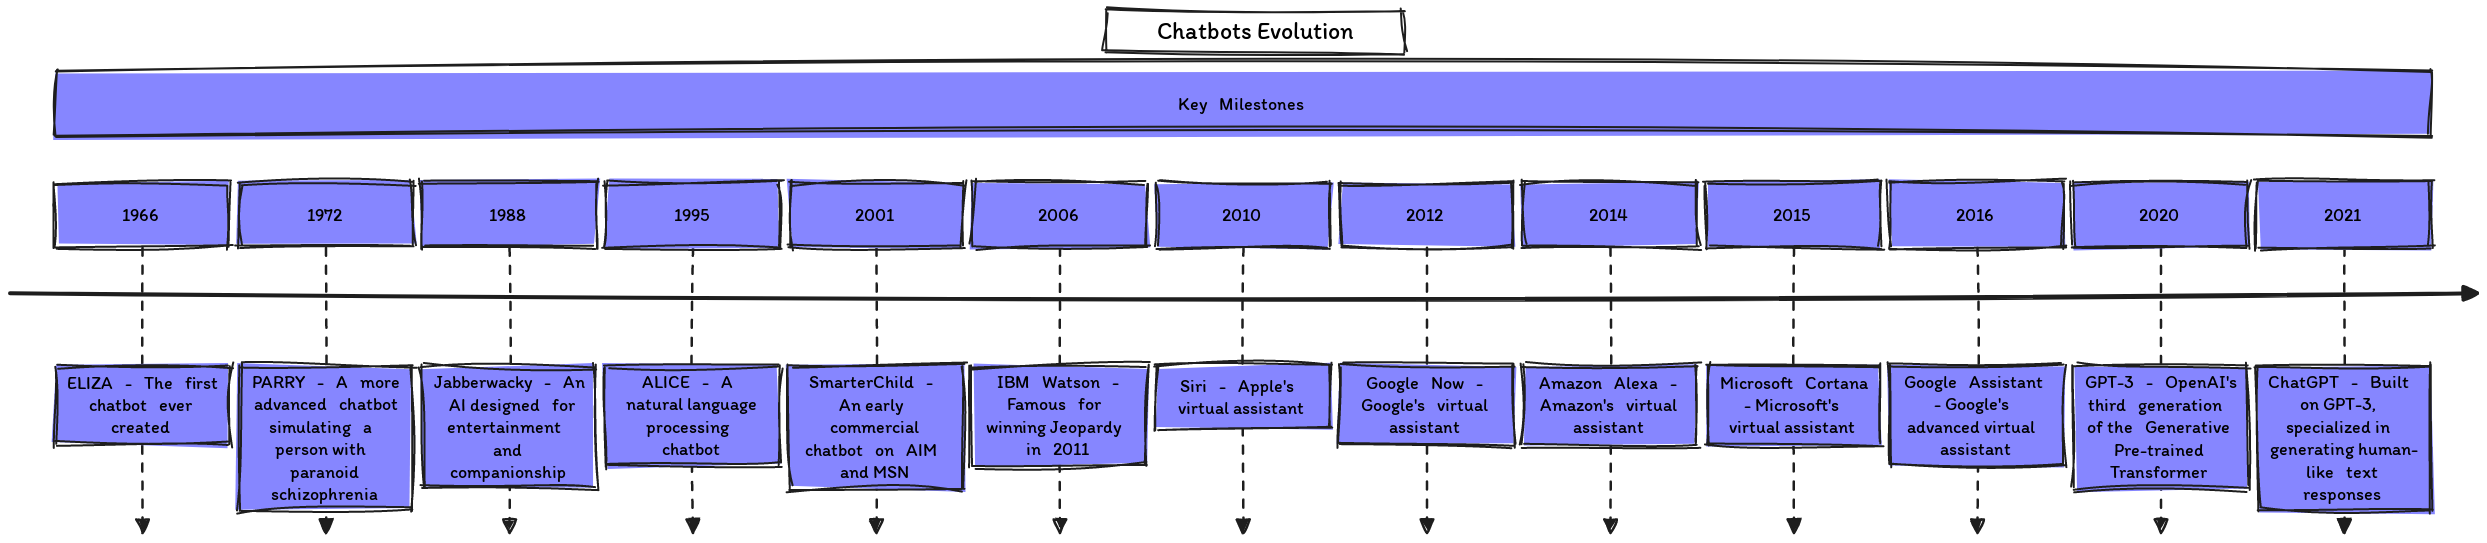
\includegraphics{images/chatbots timeline.png}
  \end{adjustbox}
  \caption{Chatbots History Timeline.}
\end{figure}

The integration of artificial intelligence (AI) into education is a major change in the way we teach and learn. Chatbots have become a key part of this change. They can automate assessments, and act as virtual assistants for educational purposes. The arrival of advanced AI chatbots, such as ChatGPT, represents a major step forward in how chatbots are used in education, improving the level of interaction and support available to both students and teachers \citep{Annuš2023}.

Chatbots are used in education for a variety of reasons, from providing Q\&A platforms to simulating conversations with successful entrepreneurs \citep{Vanichvasin2022}. A study with first-year graduate students in an entrepreneurship program showed that chatbots significantly improved learning outcomes and student satisfaction. These chatbots, designed to mimic the insights of successful entrepreneurs, responded based on real-life best practices, making the educational experience more interactive and effective \citep{Vanichvasin2022}.

The integration of ChatGPT and similar advanced chatbots into educational environments presents significant benefits, largely attributable to the substantial investments by companies in server infrastructure and data management. This enables support for millions of users simultaneously. Notably, Microsoft has recently invested \$10 billion in OpenAI, allowing for further expansion \citep{teamsilverbackMuchWill}. Such technological advancements empower the creation of educational content and the facilitation of online tutoring services. Educators can use ChatGPT's capabilities to create customized teaching aids, including quizzes, by using its custom dataset feature. This feature permits the incorporation of specific data or information, allowing ChatGPT to produce materials that align with the educators' specific curriculum requirements. \citep{Vasudevan2024}.


\subsection{Challenges in Accessing University Support Services}

In a study by \cite{Harryba2022Understanding}, it was found that international students, despite recognizing their need for help, seldom use the support services offered by universities. This reluctance is often due to language barriers and cultural differences, as well as a lack of knowledge about the services available. Similarly, the research highlighted by \cite{Abreu2016StudentExperiences} shows that students with disabilities face their own set of hurdles. Although they have disability support services (SDS) at their disposal, these students tend to engage with SDS minimally, averaging about 4.7 visits each semester.  The challenges do not stop there, especially with the rise of online and distance learning. \cite{ArkoAchemfuor2017StudentSupport} and \cite{WalkerGibbs2016ViewThrough} have both pointed out difficulties faced by students in remote or rural areas, or those enrolled in distance learning programs. Poor internet connectivity and unfamiliarity with digital platforms can make accessing digital resources and support services tricky. Lastly, navigating the wide range of resources and services offered by universities can often overwhelm students. The challenge mainly lies in the need to visit many websites and go through lots of pages to find a specific support service. This approach to getting information can lead to frustration and, sometimes, stop students from seeking the help they need. \citep{Harryba2022Understanding}.



\subsection{Academic Support and Mental Health}

The study conducted by \cite{patel2023enhancing} points out how important chatbots have become in education settings. These chatbots use specific knowledge within their domain and natural language
processing (NLP) techniques to accurately identify and respond to students’ unique needs. \cite{potts2021chatbots} looks into how chatbots could completely change mental health support, stressing that chatbots need to be both understanding and full of information. By adding engaging activities and mental health checks, these chatbots can make users more involved and offer relevant support to those dealing with mental health issues.

Adapting to the University can be challenging, leading many students to overlook their health because of academic or financial concerns. The work by \cite{kettle2023user} talk about how chatbots with dialogue-based interfaces are helpful. The research shows that the ease of access, the style of conversation, and the presence of human-like features are crucial in encouraging students to engage and maintain their well-being. Also, another study by \cite{kumar2022exploring} looks into the particular stressors for computer science students, who often face a lot of stress in competitive environments. The findings of the study
indicate that chatbots can be an effective and accessible support system for these students, overcoming the reluctance of some to use traditional support services.

\subsection{Summary}

The background section explores how chatbots have evolved in education, moving from scripted responses to complex conversations powered by AI and natural language processing. It highlights the journey from early chatbots like ELIZA to advanced systems like ChatGPT, showing how these tools have become more capable of understanding and interacting with users in a human-like way. The section also touches on the challenges students face when trying to access university support services, such as language barriers and the difficulty of navigating various resources. It points out how chatbots can help overcome these obstacles by providing support and making it easier for students to find the help they need. Overall, the section paints a picture of chatbots as a valuable tool in modern education.

\section{Similar Applications}


In this part, we'll take a closer look at four chatbot applications that are similar to GlasgowSupportBot. For each of these applications, we will give a small description, we'll explore the features, strengths, and weaknesses. 

\subsection{CSUNny}

CSUNny is a chatbot project powered by artificial intelligence, started by California State University, Northridge, and launched in 2018 \citep{csunCSUNny}. Its main goal is to boost student interaction and help achieve academic success. This project is part of the Graduation Initiative 2025 and was created to tackle the issue of increasing graduation rates within the California State University System. I took the time to chat with CSUNny, diving into its capabilities to get a feel for its offers and pinpoint its strengths, weaknesses, and features.

\begin{figure}[h!]
  \centering
  \begin{adjustbox}{center,max height=0.24\textheight, max width=\linewidth}
    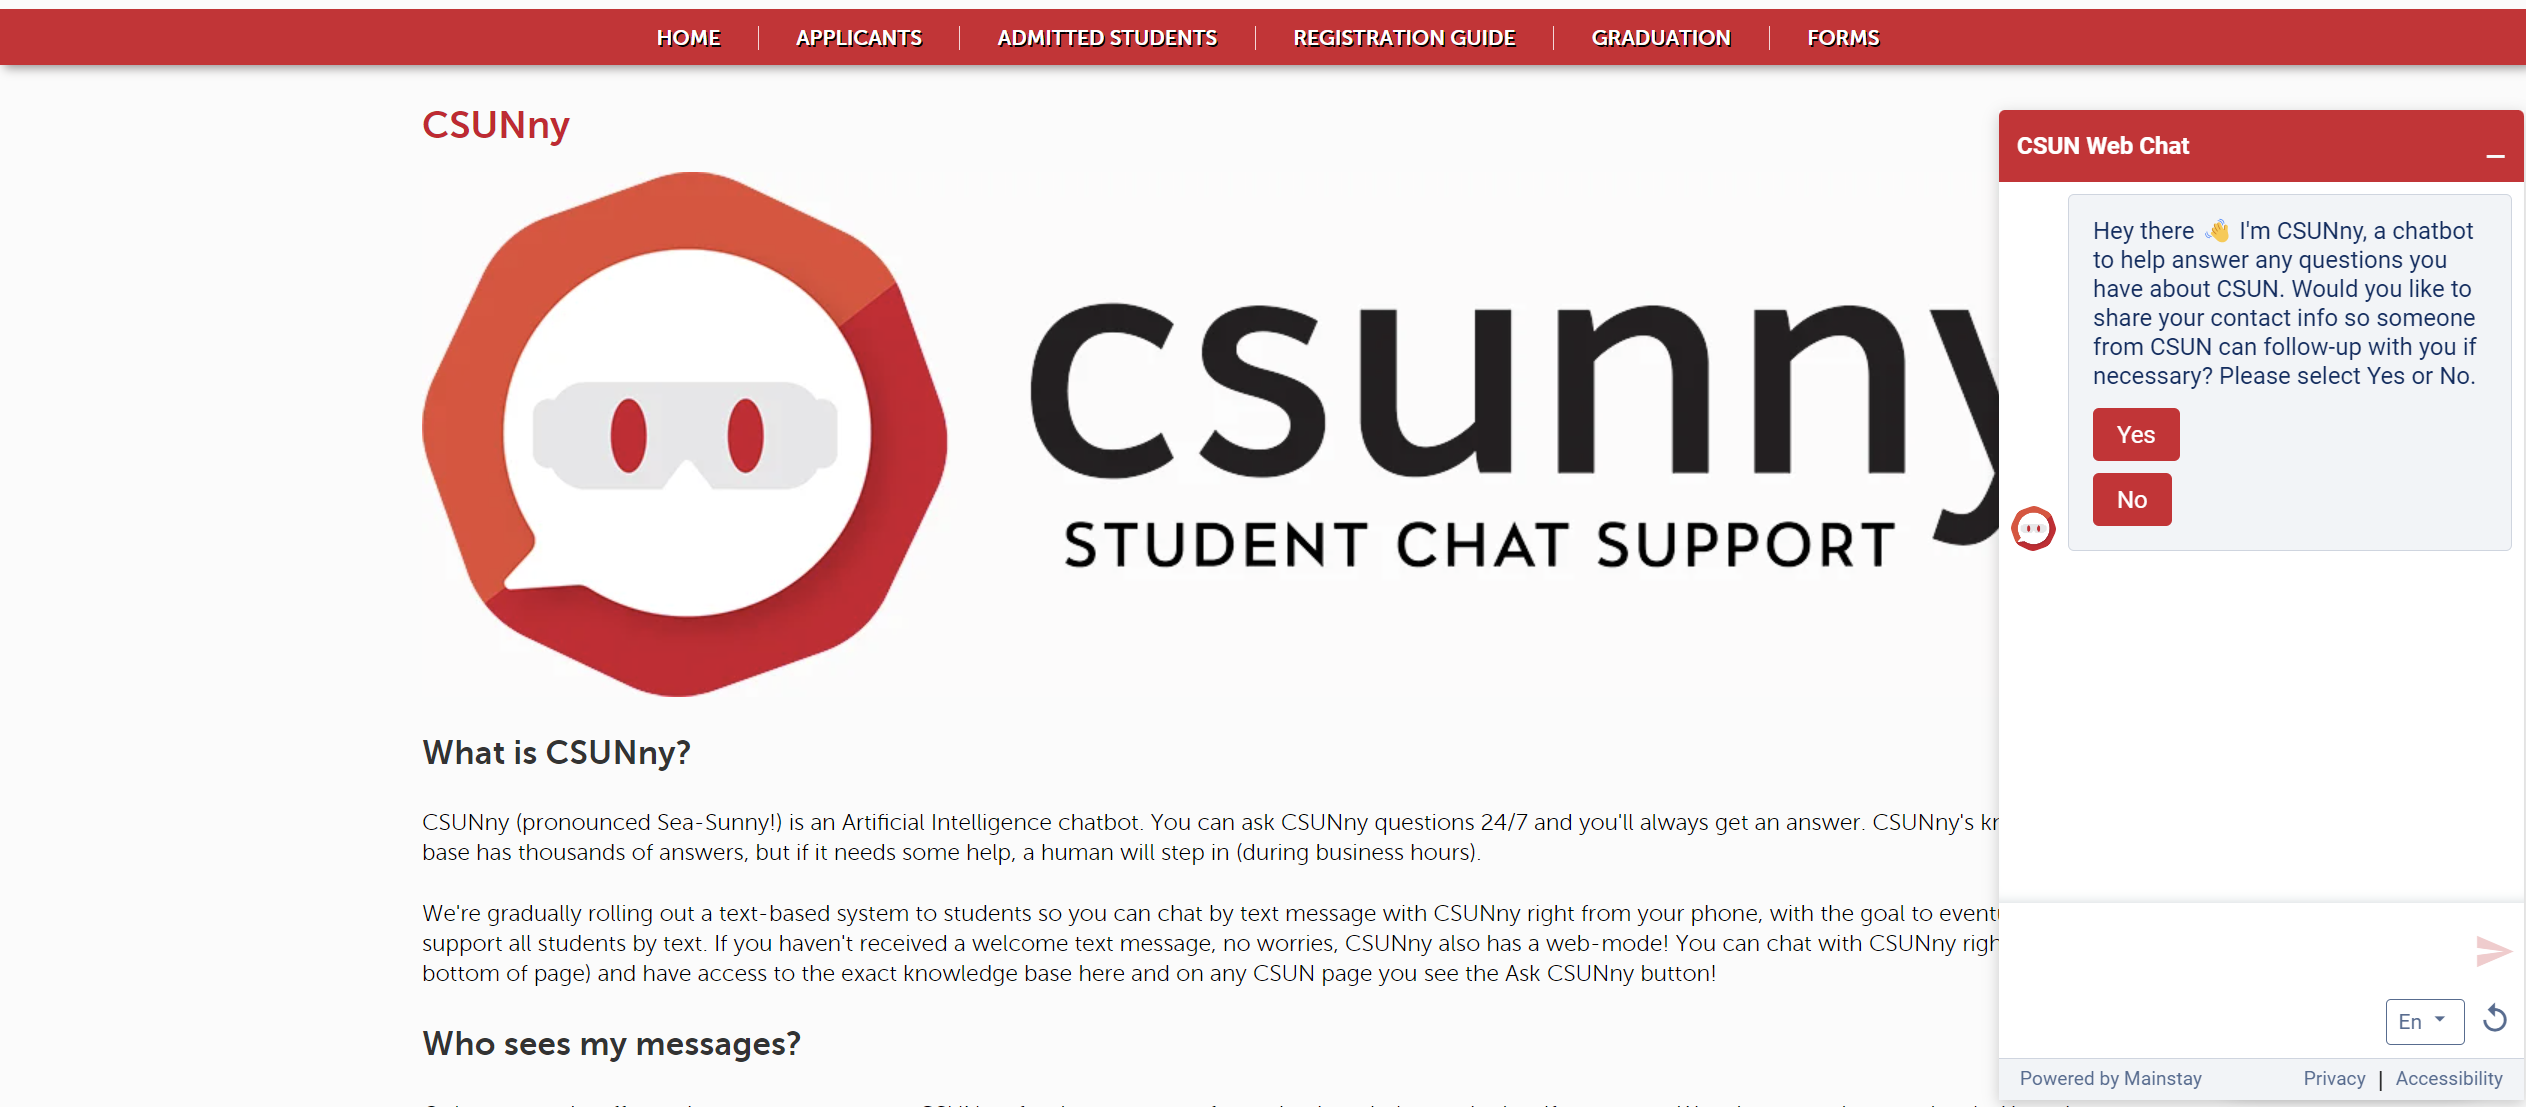
\includegraphics{images/csunny.png}
  \end{adjustbox}
  \caption{CSUNny Main Page.}
\end{figure}



\textbf{Features}

\begin{itemize}

    \item Provides 24/7 support, allowing students to seek assistance and access information anytime.

    \item For questions or concerns, students can reach out directly to CSUNny via email or contact CSUN IT for assistance.

    \item Students can choose not to receive text messages from CSUNny, with easy options to pause or stop messaging.
\end{itemize}

\textbf{Strengths}

\begin{itemize}
    \item CSUNny has been successful in improving graduation rates, demonstrating significant success in its objective to enhance student academic progression.
    
    \item CSUNny is accessible via text message and web mode, offering flexibility in how students can interact with it.

    \item With thousands of answers in its database, CSUNny can handle a wide range of queries.

    \item If CSUNny cannot answer a question, approved staff can step in during business hours to assist.

    \item Conversations with CSUNny are viewed only by approved staff, ensuring user privacy and data protection.
    
\end{itemize}

\textbf{Weaknesses}

\begin{itemize}

    \item While CSUNny has a vast knowledge base, the accuracy of its responses might vary depending on the complexity of the questions asked. Misinterpretations or outdated information could lead to incorrect guidance.

    \item The text messaging system is being gradually rolled out, meaning not all students may have access to this feature immediately.

    \item CSUNny likely lacks emotional intelligence, which can be crucial for understanding and responding to students' emotional states or providing support during stressful academic situations.

    \item The user interface (UI) of a chat does not look very good. It is important to have a good UI so that it is more engaging and intuitive for students. 

\end{itemize}

\subsection{Beacon}

In 2019, Staffordshire University launched Beacon, a friendly digital assistant designed to help students navigate university life more smoothly \citep{staffsBeaconYour}. It is a chatbot that can help you find where you need to go on campus and manage simple tasks like viewing your class schedule or getting a new student ID card. Beacon is all about making student life easier, providing instant answers to common questions, and connecting students with resources and support whenever they need it. 

\begin{figure}[h!]
  \centering
  \begin{adjustbox}{center,max height=0.34\textheight, max width=\linewidth}
    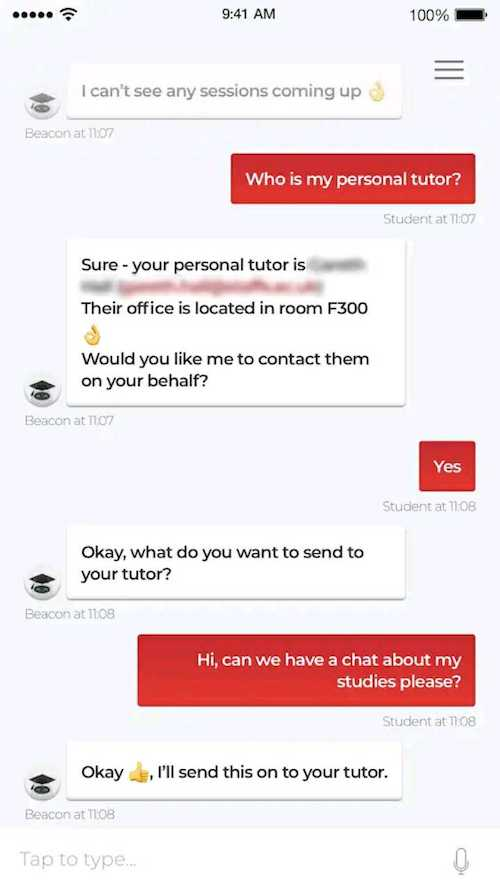
\includegraphics{images/beacon.jpg}
  \end{adjustbox}
  \caption{Beacon Chat.}
\end{figure}

\textbf{Features}

\begin{itemize}

    \item Students can view their academic schedule/timetable, helping them stay organized and prepared for their classes.

    \item Students can access the contact information of lecturers, personal tutors, and course leaders. They can also search generally for the staff directory.

    \item Beacon assists in finding societies and clubs, provides directions to rooms and places on campus, and answers common questions across various university services like Careers, Counselling, Digital, International Student, Library, Student Enabling, Student Services, and Students' Union.

    \item Students can request important documents directly through the platform.
    
\end{itemize}

\textbf{Strengths}

\begin{itemize}

   \item Beacon eases students into university life and supports them throughout their course, aiming to reduce dropout rates.
   
   \item It alerts staff with relevant experience to resolve student issues, enhancing the support system.
   
   \item  Beacon is available 24/7.

\end{itemize}

\textbf{Weaknesses}

\begin{itemize}

    \item Beacon's user interface is not very good-looking. Many helpful UI features could be added to improve the way Beacon looks.
    
    \item Beacon may still struggle with interpreting and providing accurate responses to less common or more complex queries, therefore it is better to have an approved staff to intervene during business hours.
    
    \item Data privacy and security are very important. Students might be afraid to type personal information into Beacon. Therefore it is important to establish GDPR and other regulations to ensure students feel at ease when using it.

\end{itemize}

\subsection{Deakin Genie}

Deakin Genie is a smartphone chatbot launched in 2017 \citep{deakin}. It was designed to offer information and resources to students at Deakin University. It uses a combination of natural language processing, voice recognition, and machine learning to have interactive conversations with users.

\begin{figure}[ht]
  \centering
  \begin{subfigure}[b]{0.22\textwidth}
    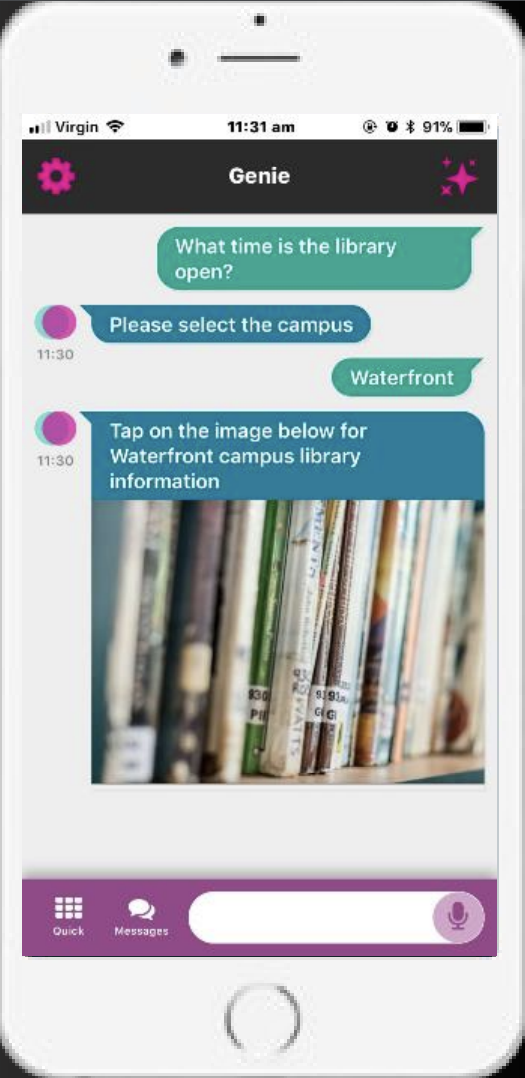
\includegraphics[width=\textwidth]{images/genie.png}
    \caption{Library Query}
  \end{subfigure}
  \hfill % Optional space between
  \begin{subfigure}[b]{0.22\textwidth}
    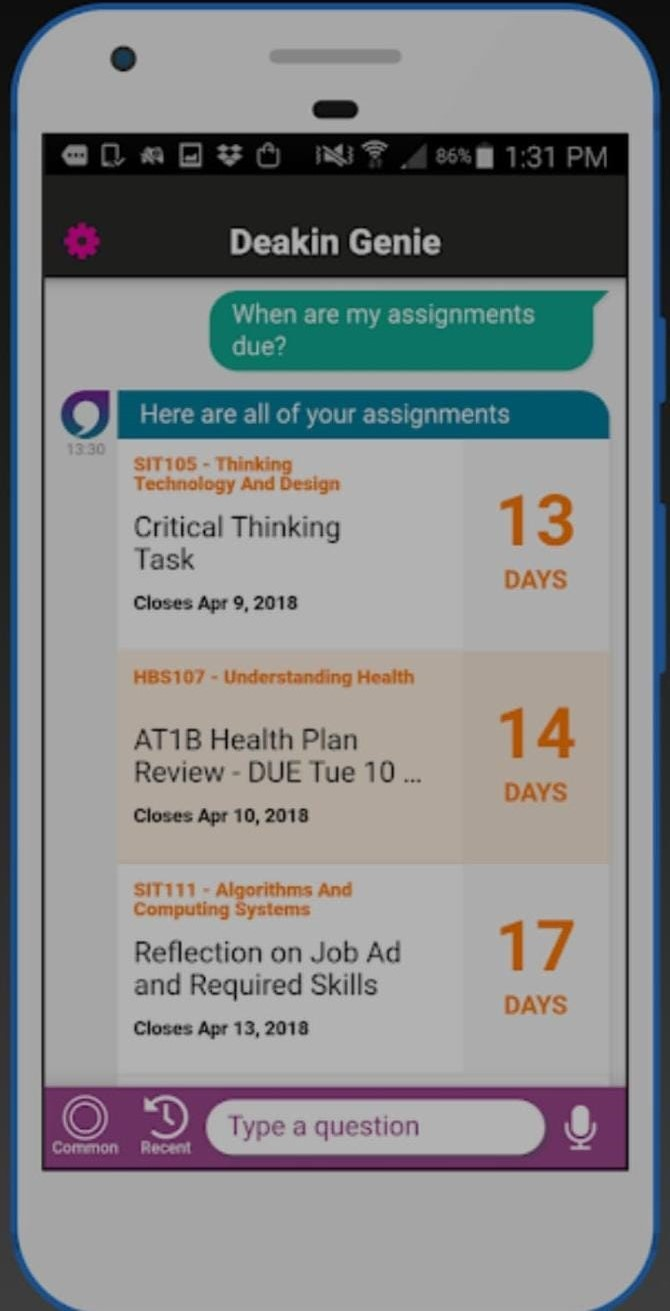
\includegraphics[width=\textwidth]{images/genie1.jpeg}
    \caption{Assignment Query}
  \end{subfigure}
  \hfill % Optional space between
  \begin{subfigure}[b]{0.22\textwidth}
    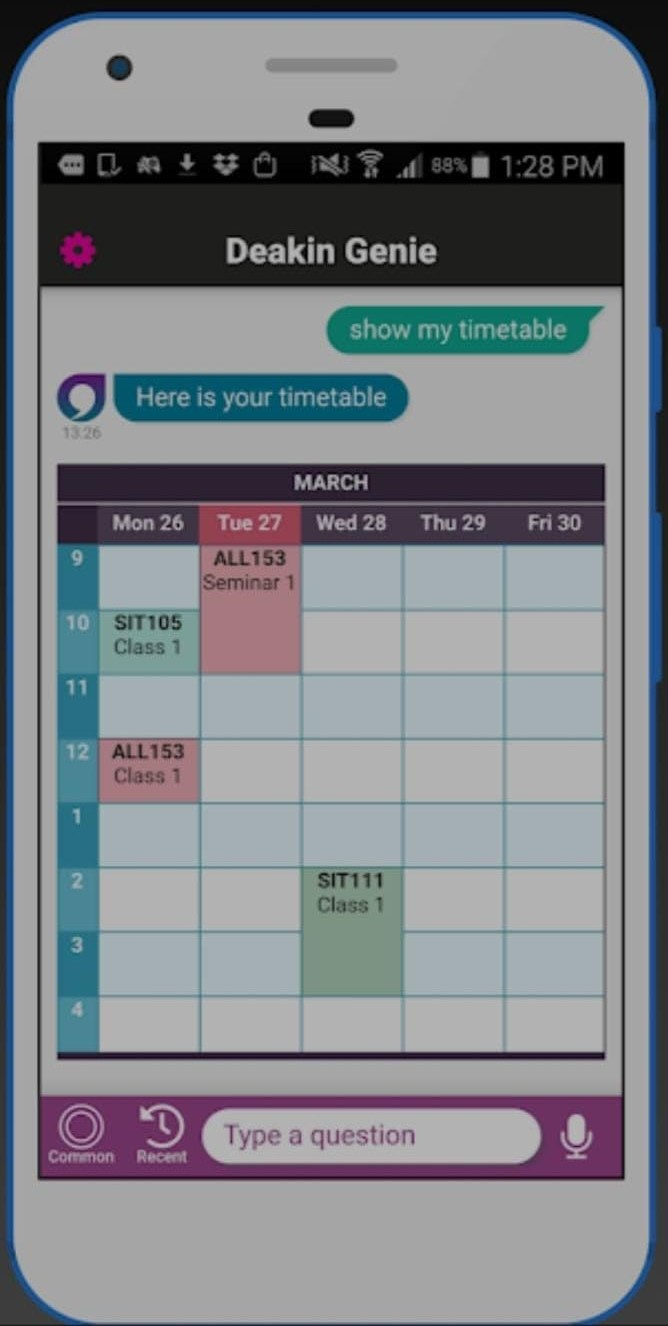
\includegraphics[width=\textwidth]{images/genie2.jpeg}
    \caption{Timetable Query}
  \end{subfigure}
\end{figure}

\textbf{Features}

\begin{itemize}

    \item  Allows for interaction through voice or text input.
    \item  Accessible via a mobile app, making it convenient for students on the go.
    \item Adapts and personalizes the experience based on individual student interactions.

\end{itemize}

\textbf{Strengths}

\begin{itemize}
    \item Deakin provides a wide range of services, from academic support to offering guidance on on-campus facilities, events, and other aspects of university life.
    
    \item Deakin automates routine inquiries and tasks, allowing university staff to focus on more complex issues.

    \item Capable of handling a large volume of queries simultaneously.
    
    \item Deakin is available 24/7.

\end{itemize}

\textbf{Weaknesses}

\begin{itemize}
    \item Some users may find navigating the app or understanding its full range of capabilities challenging without adequate guidance or tutorials.
    
    \item Requires ongoing updates and improvements to stay relevant and effective in meeting student needs.
\end{itemize}


\subsection{Pounce}

In 2016, Georgia State University launched \citep{pounce}. It is a text messaging app that supports students by offering guidance and reminders to students about critical university processes, such as enrollment deadlines and financial aid submissions. This initiative significantly reduced the occurrence of "summer melt," a situation where students accepted for admission do not proceed to enroll. Furthermore, Pounce contributed to reminding students about upcoming exams and assignments.

\begin{figure}[h!]
  \centering
  \begin{adjustbox}{center,max height=0.24\textheight, max width=\linewidth}
    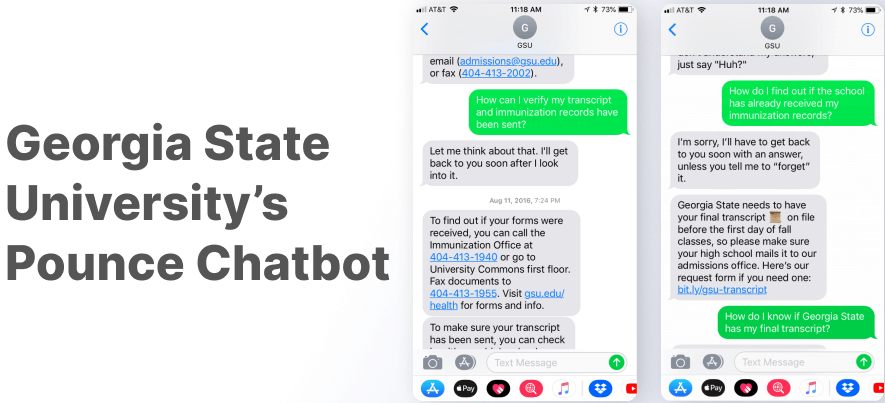
\includegraphics{images/pounce.png}
  \end{adjustbox}
  \caption{Pounce.}
\end{figure}


\textbf{Features}
\begin{itemize}

    \item Helps potential students navigate the admissions process with reminders and information on deadlines and required documents.
    
    \item Offers guidance on financial aid applications, deadlines, and eligibility requirements.
    
    \item Assists students in finding locations on campus, such as administrative offices, and classrooms.
\end{itemize}

\textbf{Strengths}

\begin{itemize}

    \item Collects data on student inquiries, which can provide valuable insights into common concerns and areas where the university might need to improve resources or communications.

    \item  Can offer support in multiple languages.
    
    \item Delivers immediate answers to frequently asked questions, reducing wait times for information.
    
\end{itemize}
   
\textbf{Weaknesses}

\begin{itemize}

    \item Collecting and processing personal information raises privacy and data protection concerns.
    
    \item As an automated tool, it struggles with complex queries.
    
\end{itemize}




%==================================================================================================================================
\chapter{Requirements}

In this chapter, we will explore the functional and non-functional requirements using the MoSCoW method. At the start of the project, some basic requirements for GlasgowSupportBot were established. However, as the development journey continued, these requirements were frequently updated. Also, we will be talking about User Personas to understand the potential use cases of the application. Then user stories will be generated from these personas. After considering all these, the final functional and non-functional requirements were established.

\section{MoSCoW Approach}
\label{ch:MoSCoW Approach}

The MoSCoW method is a prioritization technique used in project management and software development. It helps everyone involved in the project to agree on what features or tasks are essential and which ones can wait. 'MoSCoW' stands for different levels of priority:

\begin{itemize}
    \item \textbf{Must Have:} These are non-negotiable requirements critical for the system to be considered successful.
    \begin{itemize}
        \item Must be implemented for the project to be successful.
    \end{itemize}
    
    \item \textbf{Should Have:} These are important but not vital features, not as critical as the "Must Have" requirements.
    \begin{itemize}
        \item High priority but not essential for launch.
    \end{itemize}
    
    \item \textbf{Could Have:} These are desired features that could improve user experience or system efficiency but are not as important as the "Should Have" requirements.
    \begin{itemize}
        \item Nice to have but not as important as "Should Have".
    \end{itemize}
    
    \item \textbf{Won't Have:} These are the least critical, least beneficial, or most easy to leave out of the current project scope, considered for future updates.
    \begin{itemize}
        \item Identified as not necessary for the current development cycle.
        \item May be revisited in the future but is excluded from the current scope.
    \end{itemize}
\end{itemize}

\section{User Personas}


We began by brainstorming different ideas for features that users would find helpful. After this, we created personas to show how a variety of University of Glasgow students, each with their unique backgrounds and needs, would use the chatbot we're designing. They include a range of students such as international students, local students, undergraduates, postgraduates, students who are struggling with their studies, and students who need mental health support. Each Persona demonstrates the main goal of our project which is to make it easier for students to find and use the support services the University of Glasgow offers. We have created some personas here, but we have more of them in the Appendices in section \ref{ch:User Personas}.

\begin{itemize}
    \item \textbf{Elena} is in Scotland for a semester to study history. She is very excited to learn about Scottish culture and university life. Elena needs a place to stay because she is still new to the country. She also needs help understanding how the university works and wants to make friends quickly. A chatbot that could advise on these would help Elena a lot.

    \item \textbf{Tom} is studying computer science. He needs special arrangements to move around campus because he had an injury to his leg which caused him to have mobility issues. He is looking for information on buildings that are easy to access, services that can help him, and groups where he can talk to people like him. A chatbot that can support in finding these resources would make his time at university better.
    
    \item \textbf{Alex}, a first-year student, is studying late at night for an exam and suddenly has questions about the library's online resources and study materials specific to his course. Traditional university websites may not offer the immediate assistance Alex needs outside regular office hours. A chatbot, however, can provide instant answers, guiding Alex to specific online resources or past exam papers relevant to his study, regardless of the time.

    \item \textbf{Jess}, an international student, needs to find her way to a specific department for her registration and later, locate the nearest student health services. While university websites contain this information, navigating through multiple pages can be very tiring and could deter her from following up because the information required is too specific and therefore hard to find. A chatbot could instantly provide Jess with directions to the departments, along with opening hours and contact information for student health services.

    \item \textbf{Nora} is working on a big research project and feels stressed by the amount of work and the pressure to do well. She is looking for easier ways to find research materials, meet other experts in her field, and learn about writing and publishing her work. Guidance in these areas would help her succeed in her research and academic career.
\end{itemize}

\section{User Stories}

Following the creation of the user personas in the above sub-section, the following relevant user stories were created. Some are listed below and the rest are in the appendix, section \ref{ch:User Stories}. The user stories in the appendix are relevant to the user personas in section \ref{ch:User Personas}.

\subsection{What Questions Users want GlasgowSupportBot to Answer}
\begin{itemize}
    
    \item \textit{As a} chatbot user facing unforeseen academic challenges, \textit{I want} to learn how to navigate the Good Cause claim process and understand what circumstances qualify, \textit{so that} I can manage the impact on my academic performance with appropriate actions.
    
    \item \textit{As a} new international student at the university (like Elena and Jess), \textit{I want} the chatbot to provide me with immigration advice, information about the CAS process for my visa application, and guidance on adapting to UK and Scottish culture, \textit{so that} I can settle in more comfortably and focus on my studies.
    
    \item \textit{As a} chatbot user needing mental health support (potentially relevant for Nora), \textit{I want} information on how to access counseling services, crisis support, and peer wellbeing support, \textit{so that} I can navigate mental health challenges more effectively during my studies.

    \item \textit{As a} chatbot user studying computer science with specific learning difficulties (like Tom), \textit{I want} information on available assistive technology and training, \textit{so that} I can leverage these tools to overcome learning barriers and excel in my studies.
    
    \item \textit{As a} chatbot user who is an international student (like Elena and Jess), \textit{I want} detailed guidance on maintenance requirements and financial evidence needed for my Student Visa, \textit{so that} I can ensure my visa application is successful without unnecessary delays.
    
    \item \textit{As a} chatbot user experiencing a personal crisis affecting my academic work (relevant for all, but especially Nora), \textit{I want} to know the process for arranging exam accommodations and how to claim Good Cause, \textit{so that} I can focus on my wellbeing without compromising my academic progress.
    
    \item \textit{As a} late-night studier (like Alex), \textit{I want} instant advice on how to consult a General Practitioner for mental health support and access self-help resources, \textit{so that} I can manage stress and maintain mental health while preparing for exams.
    
    \item \textit{As a} chatbot user interested in networking and improving career prospects (applicable to all, particularly final-year students), \textit{I want} to know how to access Glasgow Careers Service, \textit{so that} I can connect with potential employers and enhance my career opportunities.
    
    \item \textit{As a} chatbot user with disabilities (like Tom), \textit{I want} the chatbot to guide me on how to register for support, and to inform me about the necessary documentation, \textit{so that} I can fully access the available service.
    
    \item \textit{As a} chatbot user with an interest in entrepreneurship (could be relevant for Tom, Alex, or Nora), \textit{I want} information on support available for students interested in entrepreneurship, including workshops and mentoring, \textit{so that} I can pursue my business ideas with the right resources and guidance.
    
\end{itemize}

\subsection{What features Users want GlasgowSupportBot to have}

\begin{itemize}
    \item \textit{As a} chatbot user engaged in ongoing research and requiring frequent interactions with various university services (like Nora), \textit{I want} the ability to review my past conversations with the chatbot, \textit{so that} I can easily recall advice, resources, and steps previously discussed without needing to repeat my queries.

    \item \textit{As a} chatbot user new to the university and its services (like Elena and Jess), \textit{I want} access to documentation through the chatbot as well as a list of available support services \textit{so that} I can know what to ask.

    \item \textit{As a} chatbot user encountering unique challenges or having suggestions for additional support services (like Tom or Alex), \textit{I want} the ability to easily provide feedback directly through the chatbot via a feedback button, \textit{so that} I can contribute to improving the chatbot's functionality and the overall user experience.

    \item \textit{As a} chatbot user working on a big research project and collaborating with faculty or peers (like Nora), \textit{I want} the option to export messages or conversation summaries from my interactions with the chatbot, \textit{so that} I can easily share accurate information, resources, or guidance received with my project team or advisors.
    
\end{itemize}



\section{Functional Requirements}

Functional requirements define what a product must do and what its features and functions are. The MoSCoW prioritization technique was used to prioritize the requirements. We will label the requirements as four distinct groups: 'must have', 'should have', 'could have', and 'won't have', as described in section \ref{ch:MoSCoW Approach}. Also, in Section \ref{ch:Requirements Validation}, you can see the requirements validation.

\section*{\textbf{Must Have}}

\begin{itemize}
    \item The system must be able to receive user queries and process these queries to respond.

    \item Must have the ability for users to engage in real-time conversations with the chatbot, receiving immediate responses to inquiries.
    
    \item Present information on various university support services, including mental health, disability, international student advice, and academic support.

    \item Implement natural language processing capabilities to understand and respond to inquiries effectively. LangChain library can be used.
    
    \item Ability to create and manage a database for storing and retrieving information relevant to user queries. Chroma or Redis can be used.

    \item User chat sessions are stored and can be resumed.

    \item Enable users to manage their chat histories through the front-end interface, including options to start new chats, select existing chats from history, and delete chats.

    \item Provide the ability for users to submit feedback through a form, including details like subject, name, email, and message.
    
    \item Enable users to review past conversations with the chatbot.

    \item Enable users to export chat histories as txt.

    \item Validate inputs before sending emails and queries.

    \item Proper error handling and validation in both the back-end and front-end to manage and report failures gracefully.
    
    \item Users can see the system's currently available support services information.

    \item Offer detailed guidance and documentation accessible through the chat interface.
    

\end{itemize}

\section*{\textbf{Should Have}}

\begin{itemize}
    
    \item Implement a welcome popup for first-time users.

    \item Support multiple languages to consider international students.

    \item Email integration to send feedback submissions to an administrative account for review.

    \item Use Flask and React as back-end and front-end.

    \item Encrypt the chat messages stored in local storage to protect user privacy.
    
    \item Users can see FAQ with answers.

    \item Allows users to toggle dark/light theme.

    \item Allow users to search through their chat history with advanced filtering options, such as date range, and keywords.

    \item Implement a system for users to provide direct feedback on chatbot responses (e.g., "Was this answer helpful?"), to allow for improvement of chatbot accuracy and relevance.

    \item Allow the chat to understand follow-up questions in a chat session.

    \item Allow chatting limits due to OpenAI costs.

    \item  Allow users to manage their profile information, including contact details and preferences.

    \item Implement rate limiting on the system's API to protect against abuse and ensure fair usage, particularly for integrations with external services.

\end{itemize}

\section*{\textbf{Could Have}}

\begin{itemize}
    \item Adding voice input and output capabilities to make the chatbot accessible through voice commands.

    \item  Incorporating more sophisticated natural language processing and machine learning algorithms to improve the chatbot's understanding and responses to complex queries.

    \item Capability for users to register and log in.

    \item Allowing the chatbot to understand and respond with multimedia content, such as images, videos, or documents, for more interactive and informative responses.

\end{itemize}

\section*{\textbf{Won't Have}}

\begin{itemize}

    \item  Capability to integrate with university databases or systems to provide real-time information on schedules, grades, or enrollment directly through the chatbot.

    \item Direct integration for users to chat with live human support agents through the chatbot interface. The focus remains on automated responses.

    \item The ability for the chatbot to learn and adapt its responses dynamically based on user interactions without manual updates or training.

    \item A mobile application for iOS and Android. The project focuses on a web-based solution. It can still be accessed via mobile browsers but the user interface does not suit it.

    \item A standalone mobile application version of the system.

    \item While basic accessibility is considered, extensive compliance with all levels of WCAG (Web Content Accessibility Guidelines) might not be fully implemented in the initial version.
    
\end{itemize}

\section{Non-Functional Requirements}

Non-functional requirements, on the other hand, describe the general properties of a system that GlasgowSupportBot must exhibit to ensure user satisfaction and system reliability. 

\textbf{Performance} - Responses to user queries should be timely, with minimal latency. The system should also efficiently handle multiple concurrent users without significant degradation in performance.

\textbf{Usability} - The chatbot interface should be very intuitive and easy to navigate, including those with disabilities. Also, navigating within the chat interface should be smooth, without any lag or delays moving between pages.

\textbf{Reliability} - the system must be reliable. If something occurs unexpectedly, it must handle the error and display an appropriate error message.

\textbf{Compatibility} - The system must be accessible across various devices, ensuring compatibility with Windows, MacOS, and Linux/UNIX platforms.

\section{Chapter Summary}

In this chapter, we have outlined the final functional and non-functional requirements employing the MoSCoW method. Also, we have used User Personas and User Stories to enhance our understanding and refine these requirements further. In the next chapter, the design of GlasgowSupportBot will be presented.


%==================================================================================================================================
\chapter{Design}

In this chapter, we explore the software engineering processes and practices adopted throughout the project. We delve into the Agile development methodology, with a focus on version control and weekly stand-ups. Additionally, the system architecture will be detailed, alongside various diagrams including the Entity-Relationship (ER) diagram and Activity diagram. We will also examine wireframes. Lastly, the chapter concludes with a discussion on the selection of libraries and technologies used in the development of GlasgowSupportBot.

\section{Agile Scrum Methodology}


In creating GlasgowSupportBot, the Agile Scrum method was crucial for managing the step-by-step and adaptable design and building process. I took on the roles of Product Owner, Scrum Master, and development team, using the flexibility that Scrum offers. Doing this, helped me organize the work while still allowing changes based on new feedback, improving the chatbot's features, and meeting changing needs. I followed regular steps called sprint cycles to work on the development from the first idea to adding new improvements, using Scrum techniques like planning these cycles, doing weekly stand-ups, and looking back at each cycle to see how things went and how to make the chatbot better. 


\subsection{Stand-Up Meetings}

During the development of the application, I held weekly stand-up meetings with my supervisor to discuss the project's progress. These meetings offered valuable feedback, which allowed me to either refine or change my approach. Conversations with the supervisor were documented for potential future reference. The 'meetings' folder is located inside the compressed folder. Additionally, the project tracker, and the Gantt chart, are stored in a folder named 'Plan' inside the compressed folder.

\subsection{Version Control}

A very important part of GlasgowSupportBot was using version control throughout the development process. \cite{github}, a widely recognized platform for Git repository management, was chosen to be the project's codebase. This platform provided a centralized repository for code management and offered tools for backing up progress.

Given the nature of the project, continuous integration (CI) and automated testing were very essential to maintaining code quality and ensuring reliable application performance. To this end, a CI pipeline was established within GitHub. This pipeline was configured to automatically trigger a series of actions upon each code commit to the master branch. The automated tasks included running both back-end and front-end unit tests as well as the deployment of GlasgowSupportBot.

\subsection{Issue Management}

The use of issue management throughout the stages of GlasgowSupportBot’s development ensured that it was always possible to determine exactly what had been accomplished and what remained to be done before the project was completed. As shown in Figure \ref{Issue Tracker}, a \cite{trello} board was set up with different lists of issues, grouping tasks into categories such as ‘Backlog’, ‘To Do’, ‘Doing’ and
‘Done’ to indicate the progress. This provided a clear and concise overview of the entire project. Each issue was labeled with a task category, such as 'High Priority', 'Act Soon', or 'Testing'. 

\begin{figure}[!htb]
  \centering
  \begin{adjustbox}{center,max height=0.30\textheight, max width=\linewidth}
    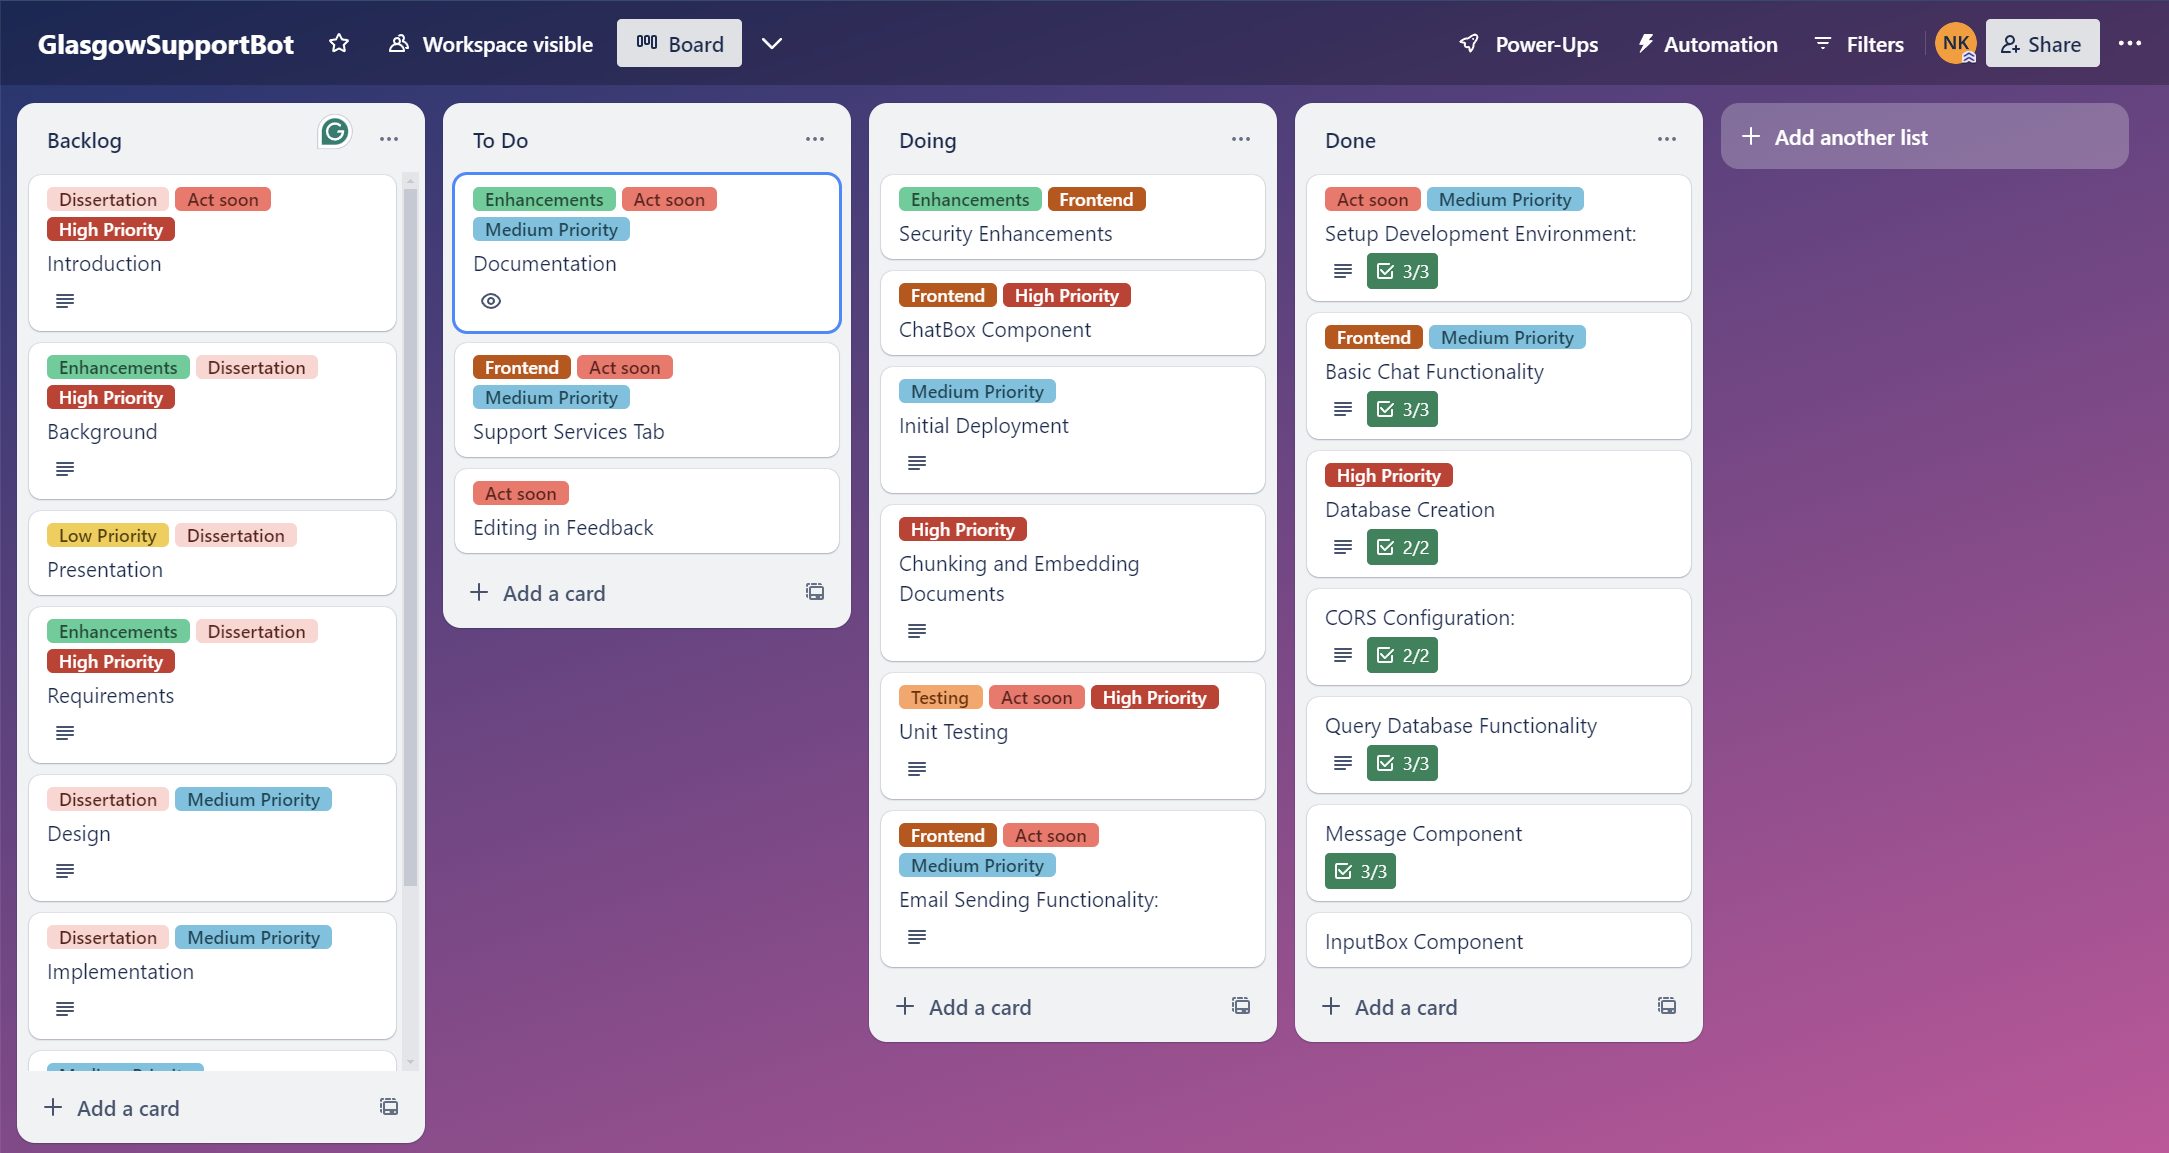
\includegraphics{images/issuetracker.png}
  \end{adjustbox}
  \caption{Trello Board. Issues are organized into lists and labeled by task type.}
  \label{Issue Tracker}
\end{figure}

\section{System Architecture}
The system architecture of GlasgowSupportBot is crucial for its operation, acting as a sophisticated framework that integrates various components to deliver both a good user experience and efficient back-end processing. This architecture is based on a three-tier design, which divides the system into presentation, application, and data layers. Each layer is designed to fulfill specific roles, ensuring a clear separation of concerns \citep{DesignStrategy}.

\textbf{Presentation Layer:} This layer is the user interface of GlasgowSupportBot, designed with React to offer an interactive and engaging user experience. It comprises components and services that work together to facilitate user interaction. Services within this layer handle server communication, and it uses Axios for efficient data exchange.

\textbf{Application Layer:} This layer serves as the core of GlasgowSupportBot's intelligence. It contains REST API controllers that act as command centers, directing requests to their appropriate destinations. Here, algorithms and processes run to determine the bot's responses to user queries, linking the user interface to the backend's data resources.

\textbf{Data Layer:} The foundation of GlasgowSupportBot is its data layer, where the Chroma Database is located. This database is essential for text processing and search indexing, enabling the bot to provide quick and accurate responses. The Data Loader in this layer ensures the database is continually updated with the latest information, allowing the chatbot to offer relevant support for university-related questions.

\begin{figure}[!htb]
  \centering
  \begin{adjustbox}{center,max height=0.30\textheight, max width=\linewidth}
    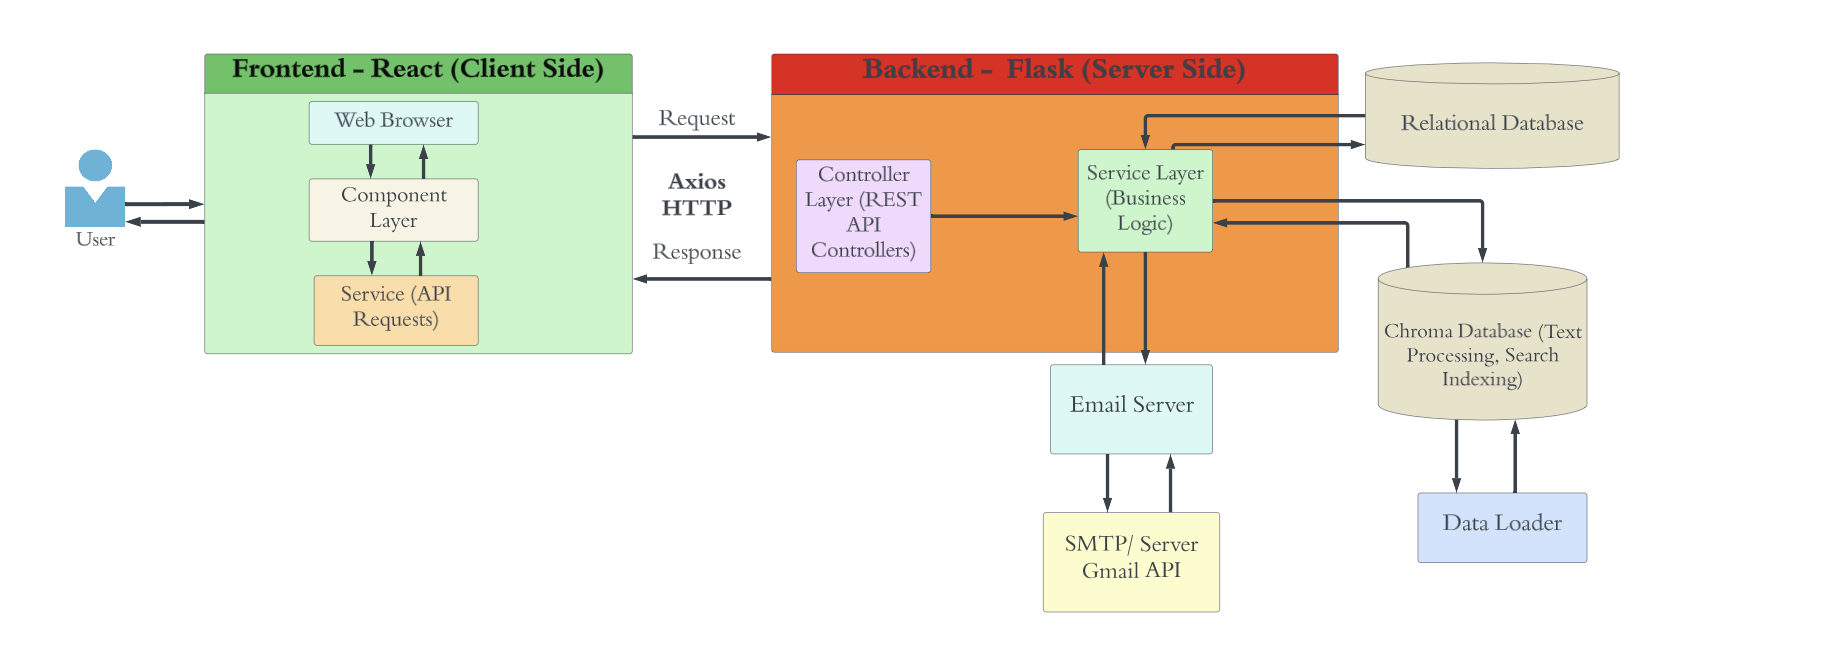
\includegraphics{images/systemarchitecture.png}
  \end{adjustbox}
  \caption{React \& Flask System Architecture Diagram.}
\end{figure}

\section*{Frontend Components}

\begin{itemize}
    \item \textbf{Web Browser:} This is where users interact with GlasgowSupportBot. The user interface is rendered in web browsers, such as Chrome and Firefox.
    
    \item \textbf{Component Layer:} This constitutes the building blocks of the front-end, and it includes various React components that make up the pages of the web application. These components are dynamically rendered which offers a responsive experience to the users.
    
    \item \textbf{Service Layer (API Requests):} Acting as the link between the front-end and back-end, this layer manages the API requests. It uses the \textbf{Axios HTTP} Library to communicate with the server.  As users engage with the chatbot, this layer is responsible for fetching and sending data back and forth.
    
\end{itemize}

\section*{Backend Components}

\begin{itemize}
    \item \textbf{Controller Layer (REST API Controllers):} This layer receives API calls from the front-end and delegates tasks based on the request's intent. It routes the calls to the appropriate services, applying the business logic correctly.
    
    \item \textbf{Service Layer (Business Logic):} This layer is the backbone of this application which processes the data according to the chatbot's logic. It interprets user queries, pulls the necessary information from the data layer, and formulates responses.
    
    \item \textbf{Email Server Integration:} This component interacts with an email service provider through the SMTP protocol and Gmail API. It is responsible for sending out emails specifically as feedback from users.
    
    \item \textbf{Chroma Database:} A vectorized database designed specifically for text processing and search indexing. It is mainly used for chatbots and it enables them to efficiently parse and search through university support content to find the most relevant information for user queries.
    
    \item \textbf{Data Loader:} This component is responsible for populating the Chroma Database with data. It ensures that the database is kept up-to-date. This also helps to give accurate and timely responses from the chatbot.
    
    \item \textbf{Relational Database:}  This SQLite database stores user-related data, such as feedback and queries. It is a structured way to store and retrieve relational data, which is different from the vectorized chroma database used for text processing and search indexing.
\end{itemize}
\section{Diagrams}

\subsection{Initial Diagrams}

Before the development of GlasgowSupportBot began, initial diagrams were created. These include a use case diagram and a sequence diagram. The design is intentionally straightforward, effectively illustrating the basic functionality of GlasgowSupportBot. These diagrams can be found in the appendices, \ref{Sequence Diagram} and \ref{Use Case Diagram} respectively.

\subsection{ER Diagram}

An Entity-Relationship (ER) diagram serves as a structured representation of the data relationships and entities involved in a database system \citep{erdiagram}. It is a crucial component in the design process which enables clear visualization of data organization and the interaction between different entities. In this project, the ER diagram focuses on key entities like users, chats, messages, and documents, along with their interrelated connections. It shows how user data is linked to chat sessions, how feedback is recorded, and how documents are processed and divided into manageable chunks for efficient retrieval and analysis. The full ER diagram and all related entities and their connections can be found in the Appendices, in section \ref{ER Diagram}. Please refer to the sample ER Diagram shown in Figure \ref{fig:ER Diagram Partial}.    

\begin{figure}[h!]
  \centering
  \begin{adjustbox}{center,max height=0.43\textheight, max width=\linewidth}
    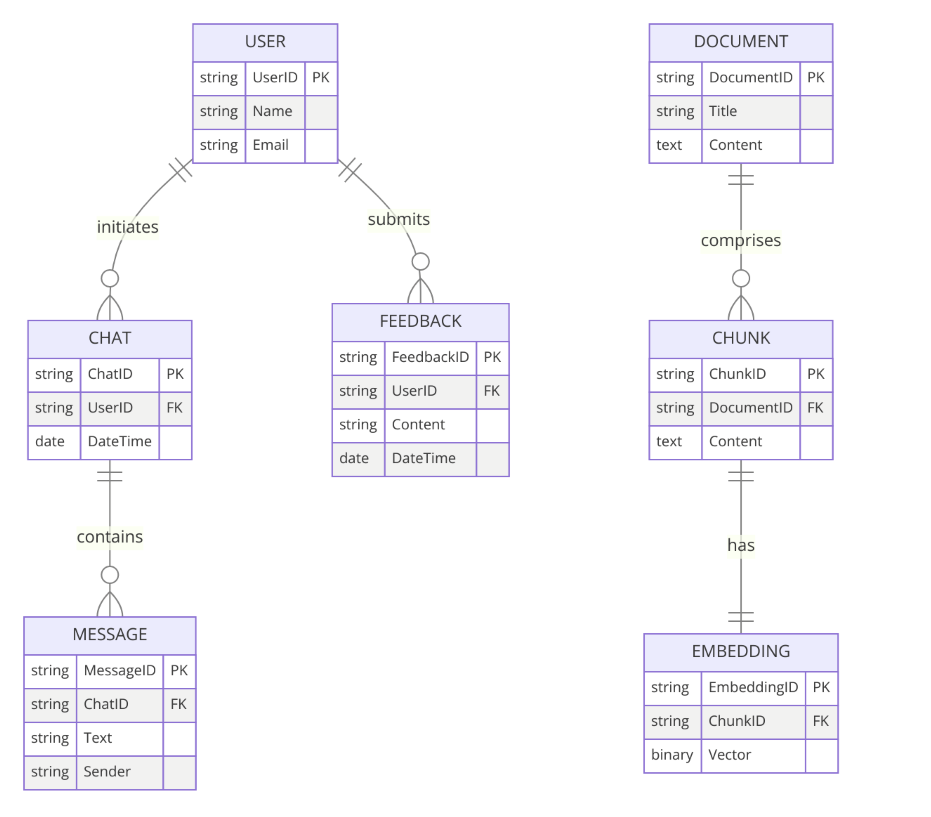
\includegraphics{images/partialerdiagram.png}
  \end{adjustbox}
  \caption{Data Model Overview.}
  \label{fig:ER Diagram Partial}
\end{figure}

\section*{Entities and Their Attributes}

\textbf{USER}: Represents the people using the bot. Each user has a unique identifier (\textbf{UserID}), a \textbf{Name}, and an \textbf{Email}.

\textbf{CHAT}: Represents a conversation session between the bot and a user. It is identified by a \textbf{ChatID} and is linked to a \textbf{UserID}. Each chat session also has a \textbf{DateTime} attribute to record when it was initiated.

\textbf{MESSAGE}: Part of the \textbf{CHAT}, this entity represents individual messages within a chat session. Each message has its unique \textbf{MessageID}, the text of the message (\textbf{Text}), and the \textbf{Sender} (who sent the message, user or AI). It is associated with a chat session via \textbf{ChatID}.

\textbf{FEEDBACK}: Represents user feedback submissions. It contains a unique \textbf{FeedbackID}, the content of the feedback (\textbf{Content}), and a \textbf{DateTime} stamp for when it was submitted. It is linked to the \textbf{USER} entity via \textbf{UserID}.

\textbf{DOCUMENT}: Contains information that the bot can draw from to answer user queries. Each document has a unique \textbf{DocumentID}, a \textbf{Title}, and the actual \textbf{Content}.

\textbf{CHUNK}: Represents a section or part of a \textbf{DOCUMENT}. This might be used to break down large documents into manageable pieces that the bot can search and analyze more efficiently. Each chunk is identified by a \textbf{ChunkID} and is related to a document via \textbf{DocumentID}. It contains its own \textbf{Content}.

\textbf{EMBEDDING}: Contains the computed vector representations of \textbf{CHUNK}s used for text similarity searches and other NLP operations. It is identified by an \textbf{EmbeddingID} and is linked to \textbf{CHUNK}s through \textbf{ChunkID}. The \textbf{Vector} is a binary representation of the chunk's content in a machine-readable format that encapsulates the meaning and context for processing.

\section*{Relationships}

\textbf{initiates}: A one-to-many relationship between \textbf{USER} and \textbf{CHAT}, indicating that a single user can start multiple chat sessions.

\textbf{contains}: A one-to-many relationship between \textbf{CHAT} and \textbf{MESSAGE}, indicating that a chat session can contain multiple messages.

\textbf{submits}: A one-to-many relationship between \textbf{USER} and \textbf{FEEDBACK}, indicating that a user can submit multiple pieces of feedback.

\textbf{comprises}: A one-to-many relationship between \textbf{DOCUMENT} and \textbf{CHUNK}, meaning that one document can be broken down into multiple chunks.

\textbf{has}: A one-to-one relationship between \textbf{CHUNK} and \textbf{EMBEDDING}, meaning that each chunk has one vector representation.

\subsection{Activity Diagram}

Activity diagrams are essentially flowcharts that depict the flow of control in a system and are a key component of the Unified Modeling Language (UML) \citep{doiDrawingActivity}. They are used to model the dynamic aspects of a system by showing the sequence of activities and the conditions that determine when and how those activities occur. They are particularly useful for visualizing the flow of a process, including parallel processes and decision points. The full Activity diagram can be found in the Appendices, in section \ref{Activity Diagram}.

\begin{figure}[h!]
  \centering
  \begin{adjustbox}{center,max height=0.40\textheight, max width=\linewidth}
    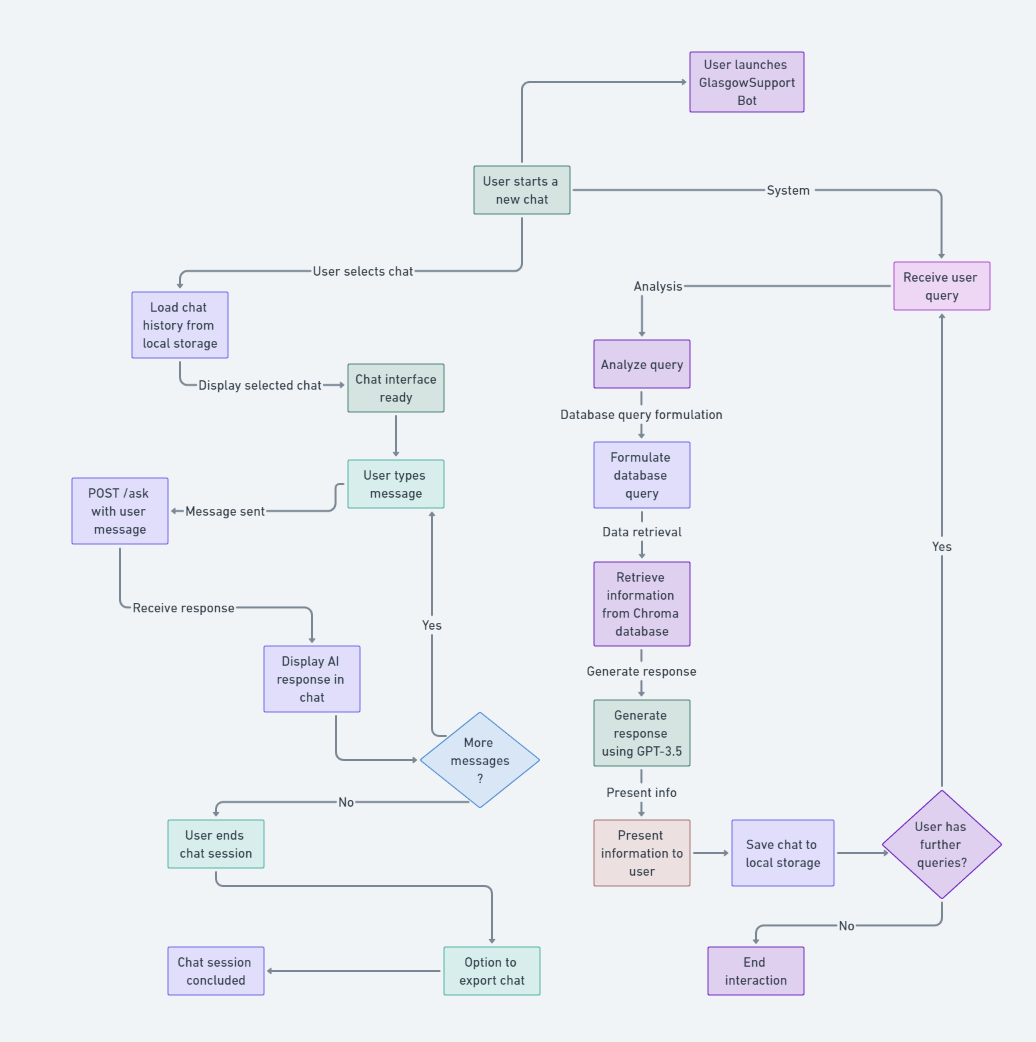
\includegraphics{images/partialactivity.png}
  \end{adjustbox}
  \caption{Activity Diagram.}
  \label{fig:Activity Diagram Partial}
\end{figure}

The activity diagram in Figure \ref{fig:Activity Diagram Partial} shows the interaction process between the user and the chatbot within the context of support services. The diagram begins with the user launching the chatbot and proceeds through various stages of interaction—from the user starting a new chat to message exchanges, and up to the conclusion of the chat session.

The diagram begins with the user launching the chatbot, and initiating a new chat. From there, it splits into two concurrent flows: the user's interaction with the chat interface and the system's process handling the user's query. As the user types and sends a message, the system analyzes the query, formulates a database request if necessary, retrieves information, and generates a response using GPT-3.5. This response is then presented to the user in the chat interface. This cycle of sending messages and receiving responses continues until the user decides to end the session. At this point, the diagram shows that the user has the option to export the chat if desired.
\section{Prototypes}

\subsection{Initial Prototypes}

Before beginning the development phase of GlasgowSupportBot, some basic prototypes were created. These prototypes are simple because they were built in the early phases. However, after defining the project's requirements, wireframes were designed and are presented in the following subsection. Access to the initial prototypes is provided in the Appendices under section \ref{Initial Prototypes}.


For instance, the main page prototype depicted in Figure \ref{fig:ProtoChatPage}, closely resembles the current version of GlasgowSupportBot but with some changes. The figure illustrates a central logo along with help and language buttons. While these elements could have been considered, it was ultimately decided to expand the "help" function through the addition of multiple tabs for a better user experience. Furthermore, language options were naturally integrated into the bot, eliminating the need for manual selection by the user. These changes indicate the project's progress and improvement since its initial prototypes.

Initially, the bot was named UGSupportbot, but it has since been renamed to GlasgowSupportBot to more accurately reflect the name of the university.

\begin{figure}[h!]
  \centering
  \begin{adjustbox}{center,max height=0.3\textheight, max width=\linewidth}
    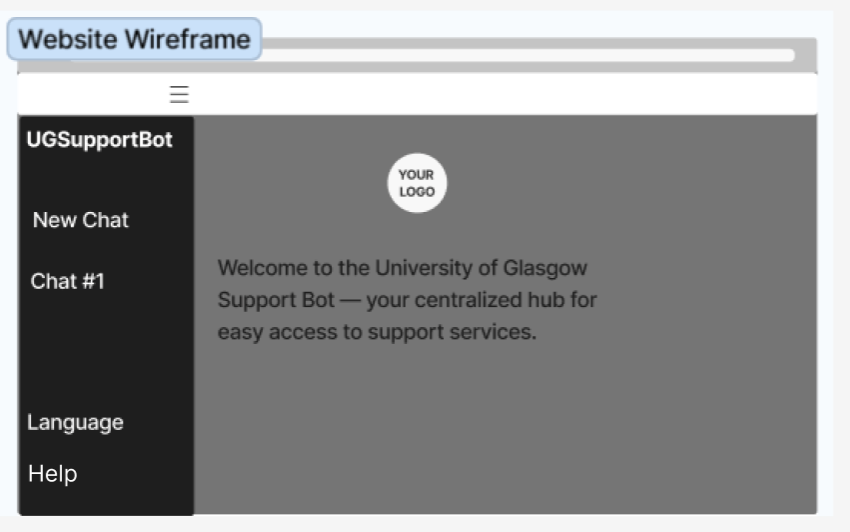
\includegraphics{images/initial1.png}
  \end{adjustbox}
  \caption{Main Prototype Page.}
  \label{fig:ProtoChatPage}
\end{figure}


\subsection{Wireframes}


Wireframes are described as schematic blueprints or plans for web pages or app screens. They are crucial for visualizing the basic structure and layout of a page or screen before detailed design and content are added \citep{wireframe}. A variety of wireframes—covering aspects such as chat, feedback, support services, documentation, and frequently asked questions—have been developed. Access to these wireframes is provided in the Appendices under sections \ref{Wireframes} \& \ref{Wireframe Software}.

For instance, the chat page wireframe is illustrated below, as depicted in Figure \ref{fig:Chat Page}. This example showcases the main chat interface, including a range of elements. Notably, it features an input box where users can pose queries related to the chatbot support services. Additionally, tabs located at the bottom left offer access to further information about the chatbot.

\begin{figure}[h!]
  \centering
  \begin{adjustbox}{center,max height=0.3\textheight, max width=\linewidth}
    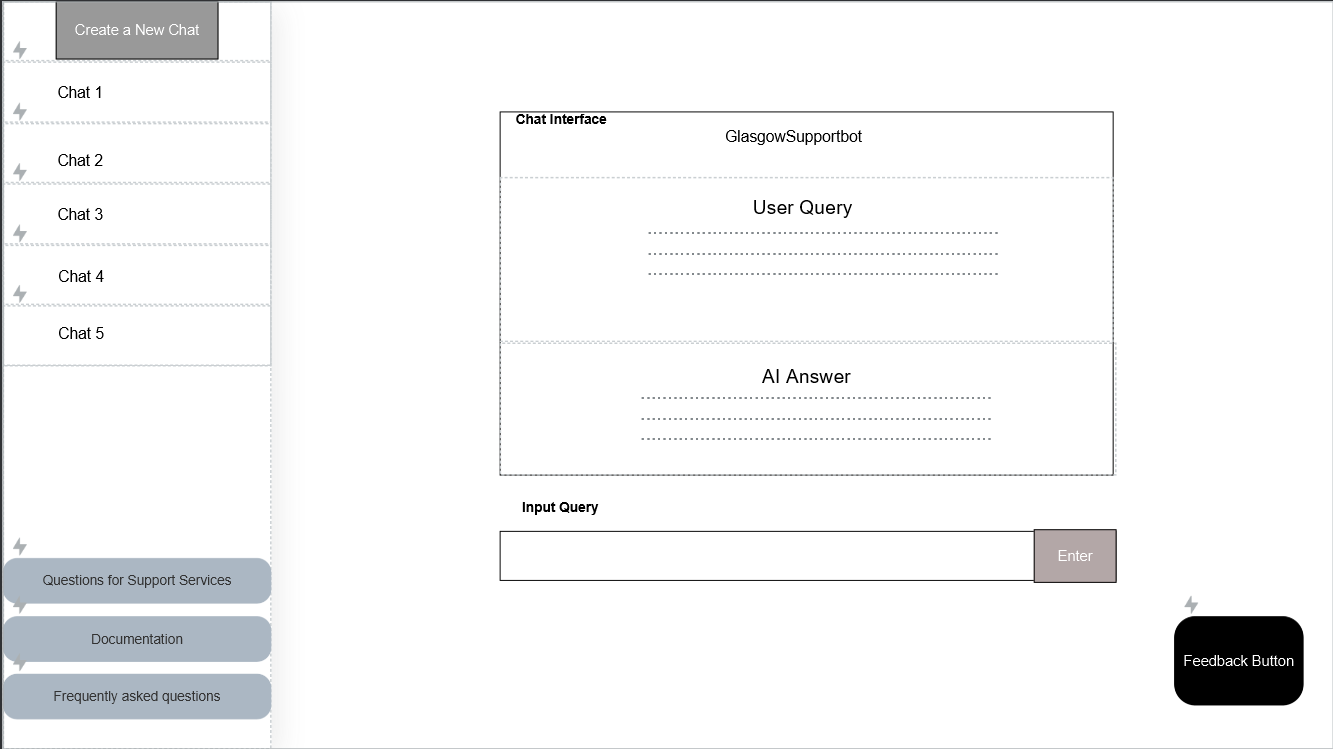
\includegraphics{images/wireframechatpage.png}
  \end{adjustbox}
  \caption{Chat Page.}
  \label{fig:Chat Page}
\end{figure}


\section{Tools and Technologies}

There are numerous libraries and technologies available for creating a chatbot web application. After conducting thorough research and experimentation, the decision was made to select the following for GlasgowSupportBot: Flask was chosen for the back-end, React alongside \textbf{AXIOS HTTP} for the front-end, and SQLite along with Chroma for the database management.


\subsection{Frontend - React}

React was chosen for GlasgowSupportBot's front-end development because of its declarative and efficient approach to designing user interfaces, especially its component-based architecture, which allows for the development of complex UIs using reusable components. This approach, along with React's virtual \textbf{DOM}, considerably improves performance, particularly for dynamic content updates that are required for a real-time chatbot web application. The decision was supported by React's extensive ecosystem, which includes tools for state management, routing, and a wide range of third-party libraries that allow for the building of a highly interactive and responsive interface. Furthermore, React's solid community support and detailed documentation make the development easier. React's smooth API and web service connections, particularly with \textbf{AXIOS} for \textbf{HTTP}, enable efficient communication with the back-end Flask server. This integration is important for submitting user queries, receiving responses, and managing user feedback within the chatbot interface. React's use of \textbf{JSX} (JavaScript XML) syntax provides a clear and concise way to describe the UI, which enhances the readability and maintainability of the code.

\subsection{Backend - Flask}

Flask, a lightweight WSGI web application framework, is chosen for the back-end of GlasgowSupportBot due to its simplicity and flexibility. It allows for quick development and easy integration with other services like Google's Gmail API for sending emails and Chroma for natural language processing and database queries. Flask's ability to handle requests efficiently and its extensive documentation make it an ideal choice for building the back-end services required for processing user queries and feedback.

The back-end structure facilitates the reception of user inputs through \textbf{RESTful APIs}. It also processes these inputs with natural language understanding and interacts with the Chroma database for fetching relevant responses. Integrating \textbf{OpenAI's API} into GlasgowSupportBot's backend greatly expands its potential. After experimenting with numerous models, including Hugging Face's transformers and other large language models (LLMs), it became clear that OpenAI's services outperformed these models in terms of response time and accuracy for a wide range of queries. This setup ensures GlasgowSupportBot can handle multiple user requests simultaneously, providing timely and accurate support to students.

\subsection{Database - Chroma \& SQLite}

The database setup utilizes both SQLite and Chroma. Chroma is a vector database and SQLite is a relational database. Vector databases handle and interpret textual data through machine learning and natural language processing. These databases convert text—ranging from individual words to complex sentences—into numerical vectors, creating a multidimensional space where each point, or vector, encapsulates the semantic meaning of the text. This allows computers to understand and process natural language by recognizing patterns, meanings, and relationships within the data, far beyond just word matching. When a query is inputted, the system translates it into a vector and compares it to the stored vectors using similarity measures, such as cosine similarity, to identify the most relevant information. 

\textbf{Chroma} was specifically chosen due to its advanced functionalities as outlined above. Vector databases are essential for enabling chatbots to process and respond to queries effectively. Unlike other data storage or caching solutions like Redis, which is known for its high-speed data handling and support for various data structures, Chroma is specifically chosen for its advanced NLP abilities to understand and accurately respond to user queries with relevant and contextually appropriate answers. Through thorough research and testing, it was determined that Chroma outperforms Redis in this regard.

\textbf{SQLite} is the preferred choice for its direct and efficient approach to data storage. It is particularly well-suited for managing user feedback and queries, ensuring smooth data operations without the need for a complex database system. Although other databases like MySQL or MongoDB could have been used, the simplicity of the data involved—mainly user feedback and queries—does not necessitate the use of these more comprehensive systems. SQLite's design is ideal for the project's needs.


%==================================================================================================================================
\chapter{Implementation}

This chapter will go over GlasgowSupportBot's features and detail how they were implemented.
The chapter will also explain the tools and libraries used to create specific functionalities, as well as solve the issues identified during the background research. Finally, the
deployment process of the web application as well as the demo will be included in this section.

\section{Receiving and Processing User Queries}

From the background research section, it was identified that students often feel overwhelmed by the vast array of resources and services offered by universities, leading to frustration and reluctance to seek help. To solve this, the feature of receiving and processing user queries through GlasgowSupportBot was created, trying to simplify access to information and make the process of seeking assistance easier.
The process for receiving and processing user queries in GlasgowSupportBot is developed by integrating Flask for back-end operations, LangChain libraries for natural language interpretation, and a Chroma vector database for contextual information retrieval. In this section, we will delve into the process of receiving and processing user queries, focusing on the technical aspects as well as the integration of these components.

\textbf{Step 1: Receiving User Queries}
\\
When a user submits a query through the GlasgowSupportBot interface, the data is encapsulated in a JSON payload and sent via a POST request to the Flask back-end, specifically to the \textbf{/ask} endpoint. This endpoint is configured in the Flask application (\textbf{app.py}) to listen for incoming queries. The JSON payload, which includes the user's query under the key 'prompt', is extracted using Flask's \textbf{request.json} method. This is shown in listing \ref{App.py Ask Endpoint.} below.


\begin{lstlisting}[language=Python, caption={App.py Ask Endpoint.}, label= {App.py Ask Endpoint.}]
@app.route('/ask', methods=['POST']) # Matching React's calling endpoint
def ask():
    data = request.json # JSON payload from React
    query = data['prompt']
    response = query_database(query)
    user_query = UserQuery(query_text=query, response_text=response)
    db.session.add(user_query)
    db.session.commit()
    return {'response': response}
\end{lstlisting}


\textbf{Step 2: Initialization of Database and Query Processing}
\\
Upon receiving a query, the first operation is to ensure that the Chroma database is initialized and ready for use. The \textbf{create\_or\_load\_database} function in \textbf{database\_creation.py} checks for the existence of the chroma database. If the database is not found, it proceeds to create a new chroma database using the function \textbf{create\_chroma\_database} by loading text documents from the "data" folder. It splits them into manageable chunks using LangChain's \textbf{RecursiveCharacterTextSplitter} method and then indexes these chunks within the database. Listings  \ref{Create / Chroma Database.}, \ref{Check existence of database.}, and \ref{Text Chunking.}, show the functions developed to check the existence of a database, construct it, and chunk text.

\begin{lstlisting}[language=Python, caption={Create / Chroma Database.}, label={Create / Chroma Database.}]
def create_chroma_database():
    directory_loader = DirectoryLoader("data", glob="*.txt") # Loading documents sitting in the directory
    docs = directory_loader.load()
    chunks = text_chunking(docs)

    # Clearing out the database
    if os.path.exists(THE_CHROMA_PATH): #checking is chroma database exists
        shutil.rmtree(THE_CHROMA_PATH)

    # Print the length of chunks for debugging
    print(f"Number of chunks before saving to Chroma: {len(chunks)}")

    if len(chunks) > 0:
        # Create new database from the documents.
        database = Chroma.from_documents(chunks, OpenAIEmbeddings(), persist_directory=THE_CHROMA_PATH)
        database.persist()
        print(f"Saved {len(chunks)} chunks to {THE_CHROMA_PATH}.")
    else:
        print("No chunks to save to Chroma.")
\end{lstlisting}

\begin{lstlisting}[language=Python, caption={Checks existence of database.}, label={Check existence of database.}]
def create_or_load_database(THE_CHROMA_PATH):
    # Find subdirectory with random name in the chroma directory
    subdirectories = glob(os.path.join(THE_CHROMA_PATH, '*'))
    
    # Check if there are any subdirectories, which implies the database exists
    if not subdirectories:
        print("No Chroma database found, creating one...")
        create_chroma_database() # generate database if not exists
    else:
        print(f"Chroma database found in: {subdirectories[0]}")
\end{lstlisting}

\begin{lstlisting}[language=Python, caption={Text Chunking.}, label={Text Chunking.}]
def text_chunking(docs: list[Document]):
    splitter = RecursiveCharacterTextSplitter(
        chunk_size=5000,
        chunk_overlap=300,
        length_function=len,
        add_start_index=True,
    )
    chunks = splitter.split_documents(docs)
    return chunks
\end{lstlisting}




\textbf{Step 3: Semantic Processing and Context Retrieval}
\\
With the database ready, the query text is then processed using LangChain's \textbf{OpenAIEmbeddings} to generate a semantic embedding. This embedding represents the query in a high-dimensional vector space, capturing its semantic variations. The vector is used to perform a similarity search in the chroma database, identifying the most relevant document chunks to the query's context. 


\textbf{Step 4: Generating a Response}
\\
The relevant document chunks obtained from the chroma database are then compiled into a coherent context, which is used alongside the original query to construct a prompt for LangChain's \textbf{ChatOpenAI} model. This model, trained on vast amounts of text data, utilizes the provided context and the query to generate a response that is both informative and contextually relevant. The use of a templated prompt ensures that the model's response is directly focused on answering the user's query, based on the context derived from the chroma database. Finally, the generated response is sent back through the Flask \textbf{/ask} endpoint to the user's interface. Listing \ref{Similarity Search, Embeddings, and OpenAI Model.} illustrates the similarity search described in Step 3, as well as the use of \textbf{OpenAIEmbeddings} as \textbf{Embeddings}. It also depicts the \textbf{ChatOpenAI} model functioning as \textbf{AI Responder} to generate responses from OpenAI.


\begin{lstlisting}[language=Python, caption={Similarity Search, Embeddings, and OpenAI Model.}, label={Similarity Search, Embeddings, and OpenAI Model.}]
embedder = Embeddings()
vector_store = VectorDB(persist_directory="chroma", embedding_function=embedder)

# Execute a similarity search within the database for the given query text, limiting results to top 2 matches.
search_results = vector_store.similarity_search_with_relevance_scores(query_text, k=2)

# Initialize the chat model for generating the answer based on the constructed prompt.
chat_model = AIResponder()
\end{lstlisting}

\section{Real-Time Conversations and Immediate Responses}

From the background research, challenges in accessing university support services, especially for international students and those with disabilities, were highlighted due to language barriers, cultural differences, and a lack of knowledge about the services available. To solve this, the real-time conversations and immediate response feature in GlasgowSupportBot was developed to offer a more accessible and immediate support channel for all students, irrespective of their background. Multiple languages were incorporated to help include everyone.
At the heart of the real-time conversation feature is the \textbf{ChatBox.js} component. It serves as the primary interface for user interaction. This component manages the state of messages within a chat session, including both user and AI-generated messages. It uses React's useState and useEffect hooks for state management and side effects, ensuring that the user interface remains responsive and up-to-date with the conversation's current state.

The \textbf{sendMessage} function is triggered when a user submits a message. This function first checks if the conditions are appropriate for sending a message (e.g., the chat is not set to read-only, and the AI is not already processing another request). It then updates the local state with the new user message, visually appending it to the chat window immediately, thus maintaining the illusion of a real-time conversation. Following the update of the local message state, the \textbf{sendMessage} function initiates an asynchronous POST request to the back-end Flask server using Axios. This request targets the \textbf{/ask} endpoint, carrying the user's message as a JSON payload. Flask uses \textbf{CORS} (Cross-Origin Resource Sharing) which allows the front-end hosted on a different origin to communicate easily with the back-end.

\begin{lstlisting}[language=Python, caption={sendMessage Function}]
const sendMessage = async (userMessage) => {
  if (readOnly || !activeChat || isAITyping) return; // Check if AI is already processing
  setIsAITyping(true); // AI starts processing
  const userMessageObj = { text: userMessage, sender: 'user' };
  setMessages([...messages, userMessageObj]);
  activeChat.messages.push(userMessageObj);

  try {
    const response = await axios.post(`${process.env.REACT_APP_API_URL}/ask`, { prompt: userMessage });
    const aiMessageObj = { text: response.data.response.trim(), sender: 'ai' };
    setMessages(messages => [...messages, aiMessageObj]);
    activeChat.messages.push(aiMessageObj);
  } catch (error) {
    console.error("Error sending message:", error);
    const errorMessageObj = { text: "Error getting response.", sender: 'ai' };
    setMessages(messages => [...messages, errorMessageObj]);
    activeChat.messages.push(errorMessageObj);
  } finally {
    setIsAITyping(false); // AI finishes processing
  }
};

useEffect(() => {
  messagesEndRef.current?.scrollIntoView({ behavior: "smooth" });
}, [messages]);
\end{lstlisting}


The Axios POST request in the \textbf{sendMessage} function is wrapped within a try-catch block to handle potential errors gracefully. Upon successful receipt of the AI's response from the back-end, the message state is updated again to include the AI's message. This update triggers a re-render of the ChatBox component, visually appending the AI's response to the chat. Should there be an error in processing the request, an error message is appended to the conversation instead, informing the user of the issue.

To ensure the chat window automatically scrolls to the latest message, a \textbf{useRef} hook is used to create a mutable reference (messagesEndRef) to the chat window's end. The \textbf{useEffect} hook then monitors changes to the message array, and upon detecting an update, executes a scroll action that brings the latest message into view, enhancing the user experience by keeping the conversation flow visible.

\section{Support Services Information Retrieval}
\label{Support Services Information Retrieval}

The presentation of university support services information within GlasgowSupportBot relies heavily on its ability to dynamically load and process data about these services. Two considerations influence the role in the bot's development and operational efficiency: the costs associated with using OpenAI models for data processing, as well as the flexibility of including data types other than plain text.

\textbf{Cost Implications of Using OpenAI Models}

The use of \textbf{OpenAI's} language models to parse and analyze university support services information adds a cost dimension to GlasgowSupportBot's operations. While the LangChain library, in conjunction with the Chroma database, significantly improves the retrieval and processing of relevant data, each interaction with \textbf{OpenAI's} models costs money. However, practical usage and testing have shown that the cost remains low. Despite making over 400 API requests to the \textbf{OpenAI} service to process user questions and provide responses, the total cost did not exceed 0.3£. This cost-effectiveness is extremely important, especially when growing the bot's usage to accommodate more users and perhaps handle a higher volume of data.

\begin{figure}[ht]
  \centering
  \begin{subfigure}[b]{0.495\textwidth}
    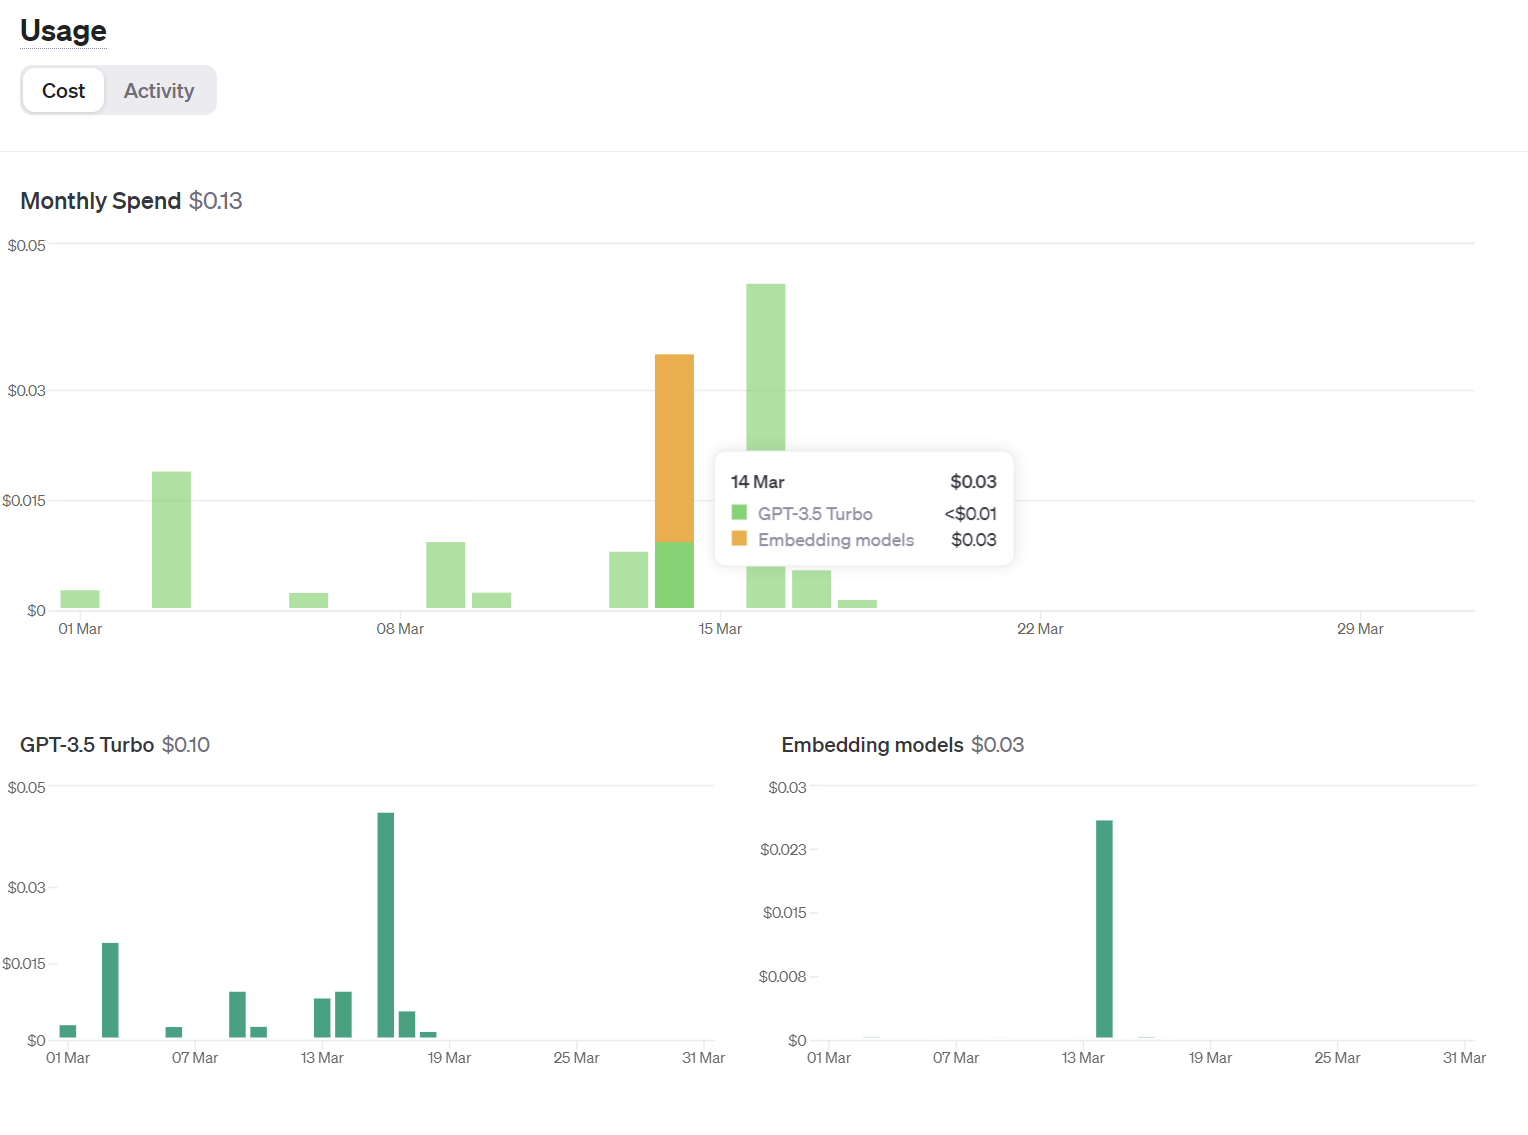
\includegraphics[width=\textwidth]{images/costopenai.png}
    \caption{OpenAI Costs}
  \end{subfigure}
  \hfill % Optional space between
  \begin{subfigure}[b]{0.495\textwidth}
    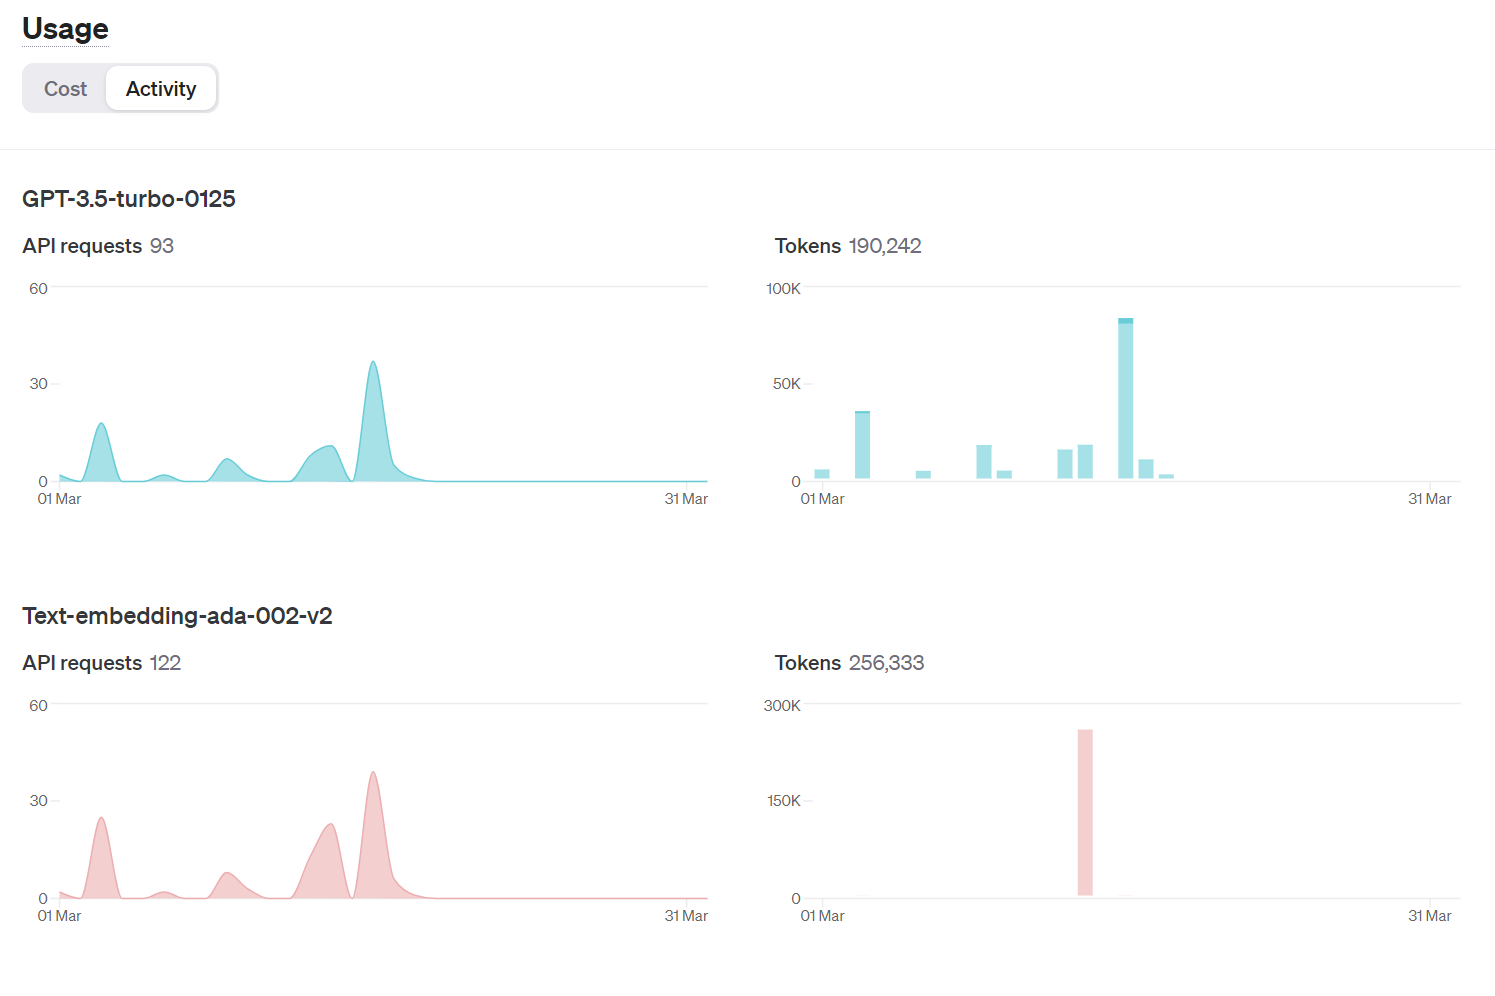
\includegraphics[width=\textwidth]{images/usageopenai.png}
    \caption{OpenAI Activity}
  \end{subfigure}
\end{figure}

\textbf{Diverse Data Formats and Flexibilities}

Currently, GlasgowSupportBot's knowledge base is populated through the \textbf{DirectoryLoader} function, focusing on \textbf{.txt} files located in the "data" folder. However, the \textbf{DirectoryLoader} function is also capable of working with multiple other data formats, such as \textbf{.pdf} and \textbf{.csv}. Presently, the data is provided in six languages, using six different \textbf{.txt} files. All the support services are consolidated into one text file for each language. For improved data organization, each university support service could be detailed in separate \textbf{.txt} files within the "data" folder. Splitting the data into individual files for services such as mental health support, academic advising, and international student services, would enhance the manageability of the information stored in the "data" folder and improve the bot's capacity to deliver precise and relevant responses.

\begin{figure}[!h]
  \centering
  \begin{adjustbox}{center,max height=0.28\textheight, max width=\linewidth}
    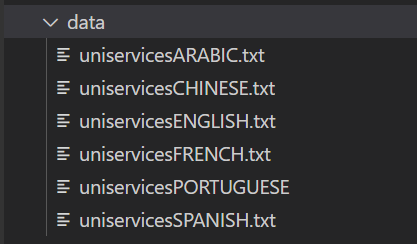
\includegraphics{images/datafolder.png}
  \end{adjustbox}
  \caption{Data Files.}
  \label{fig:Data Files.}
\end{figure}

\begin{lstlisting}[language=Python, caption={DirectoryLoader}]
directory_loader = DirectoryLoader("data", glob="*.txt") 
docs = directory_loader.load()
\end{lstlisting}

Moreover, the flexibility of the \textbf{DirectoryLoader} function and the Chroma database means that the scope of data GlasgowSupportBot can handle is not limited to support services. It can be extended to include a vast array of university-related information, from MyCampus FAQs to general university queries, essentially any data that can be formatted and saved as text. This can allow GlasgowSupportBot to serve as a centralized information hub for the entire University of Glasgow community.

\section{Chat History Management}

The Chat History Management feature in GlasgowSupportBot is a subtle approach to improving user experience by allowing users to create, review, and remove chat sessions. This functionality is connected to the bot's React front-end, particularly through the \textbf{ChatHistory.js} component, and it uses powerful encryption techniques to protect user privacy and data. This section looks into the encryption/decryption techniques, their critical role in chat history management, and the creation and deletion of chat sessions, demonstrating how they interact with the entire application architecture as defined in \textbf{App.js}.

The \textbf{CryptoJS} library's implementation of \textbf{AES} encryption and decryption is critical to ensuring the integrity and secrecy of chat histories kept locally. When a chat history is saved, each chat session data structure is first serialized into a JSON string, then encrypted with \textbf{AES} and a secret key (obtained from environment variables for security). This procedure generates ciphertext, securely kept in the browser's local storage, reducing the dangers associated with unwanted data access. When viewing chat history, the saved ciphertext is decrypted and converted back into a readable JSON format, allowing the reconstruction of the original chat session data. 

The \textbf{ChatHistory.js} component enables users to initiate new chat sessions and manage existing ones. The creation of a new chat session is triggered by user interaction, generating a unique identifier for the session based on the current timestamp and appending it to the existing chat history array. This array is then encrypted and saved back to local storage, reflecting the new state. Deleting a chat session involves filtering the chat history array to remove the specified session, followed by re-encryption and storage update. 

\begin{lstlisting}[language=Python, caption={Encryption and Decryption Functions}]
import React, { useState, useEffect } from 'react';
import CryptoJS from 'crypto-js';

const secretKey = process.env.REACT_APP_ENCRYPT_SECRET_KEY; // Secure, randomly generated key here

// Function to encrypt data before storing it
const encryptData = (data) => {
    const ciphertext = CryptoJS.AES.encrypt(JSON.stringify(data), secretKey).toString();
    return ciphertext;
};

// Function to decrypt data after retrieving it
const decryptData = (encryptedData) => {
    try {
        const bytes = CryptoJS.AES.decrypt(encryptedData, secretKey);
        const decryptedData = bytes.toString(CryptoJS.enc.Utf8);
        return JSON.parse(decryptedData);
    } catch (error) {
        console.error("Error decrypting chat history:", error);
        return []; // Return an empty array or some default state in case of error
    }
};
\end{lstlisting}

The Chat History Management functionality integrates well with other GlasgowSupportBot components thanks to \textbf{App.js}. \textbf{App.js} coordinates the interaction of the Chat History component with other sections of the application, such as \textbf{ChatBox.js}, \textbf{Documentation.js}, and \textbf{Feedback.js}, by utilizing React Router for navigation and state management hooks. This connection allows users to easily move between the bot's numerous features, such as accessing, reviewing, and exporting chat history. 

\section{Feedback Submission System}

From the background research, the importance of adapting support systems to meet student's unique needs and encourage engagement was emphasized, especially in maintaining well-being and offering support to those dealing with mental health issues. To solve this, the feedback submission system within GlasgowSupportBot was created, facilitating direct communication between users and the support team to continuously improve and tailor the bot’s services to student needs.
The feedback submission system within GlasgowSupportBot is a comprehensive feature, designed to facilitate direct communication between users and the support team regarding user experiences, suggestions, and potential issues. This system is constituted by two primary components: a front-end form implemented in \textbf{Feedback.js} for gathering user input and a Flask back-end endpoint (\textbf{/send-email} in \textbf{app.py}) responsible for processing this input and forwarding it as an email to the support team for review.

On the user interface side, \textbf{Feedback.js} presents a structured form where users can detail their feedback, including specifics such as subject, name, email, and the feedback message. This design ensures that users can easily communicate their thoughts directly within the GlasgowSupportBot interface, enhancing user engagement and providing valuable insights for continuous improvement.


\begin{figure}[ht]
  \centering
  \begin{subfigure}[b]{0.45\textwidth}
    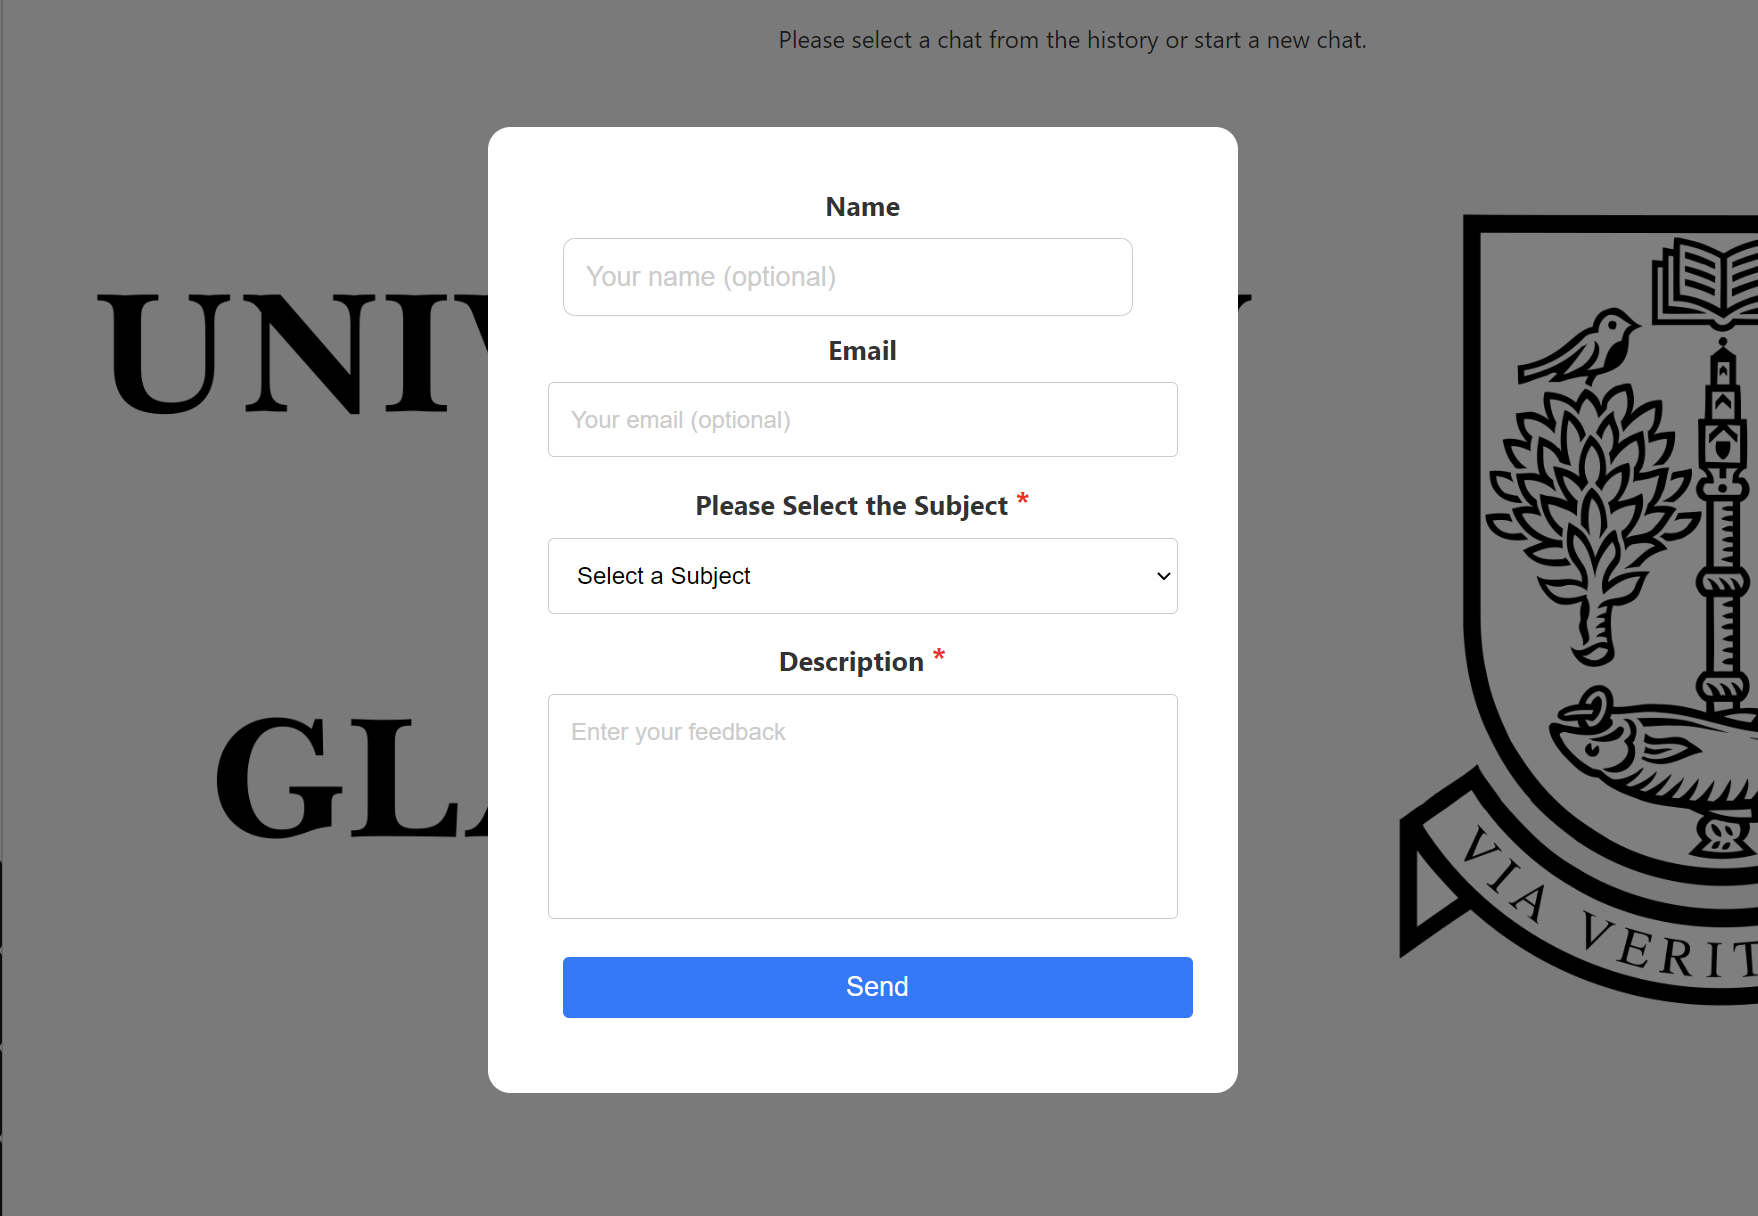
\includegraphics[height=1.75in]{images/feedbackui.png} % Adjust the height as needed
    \caption{Feedback fields.}
    \label{fig:feedback_fields}
  \end{subfigure}
  \hfill % Optional space between
  \begin{subfigure}[b]{0.5\textwidth}
    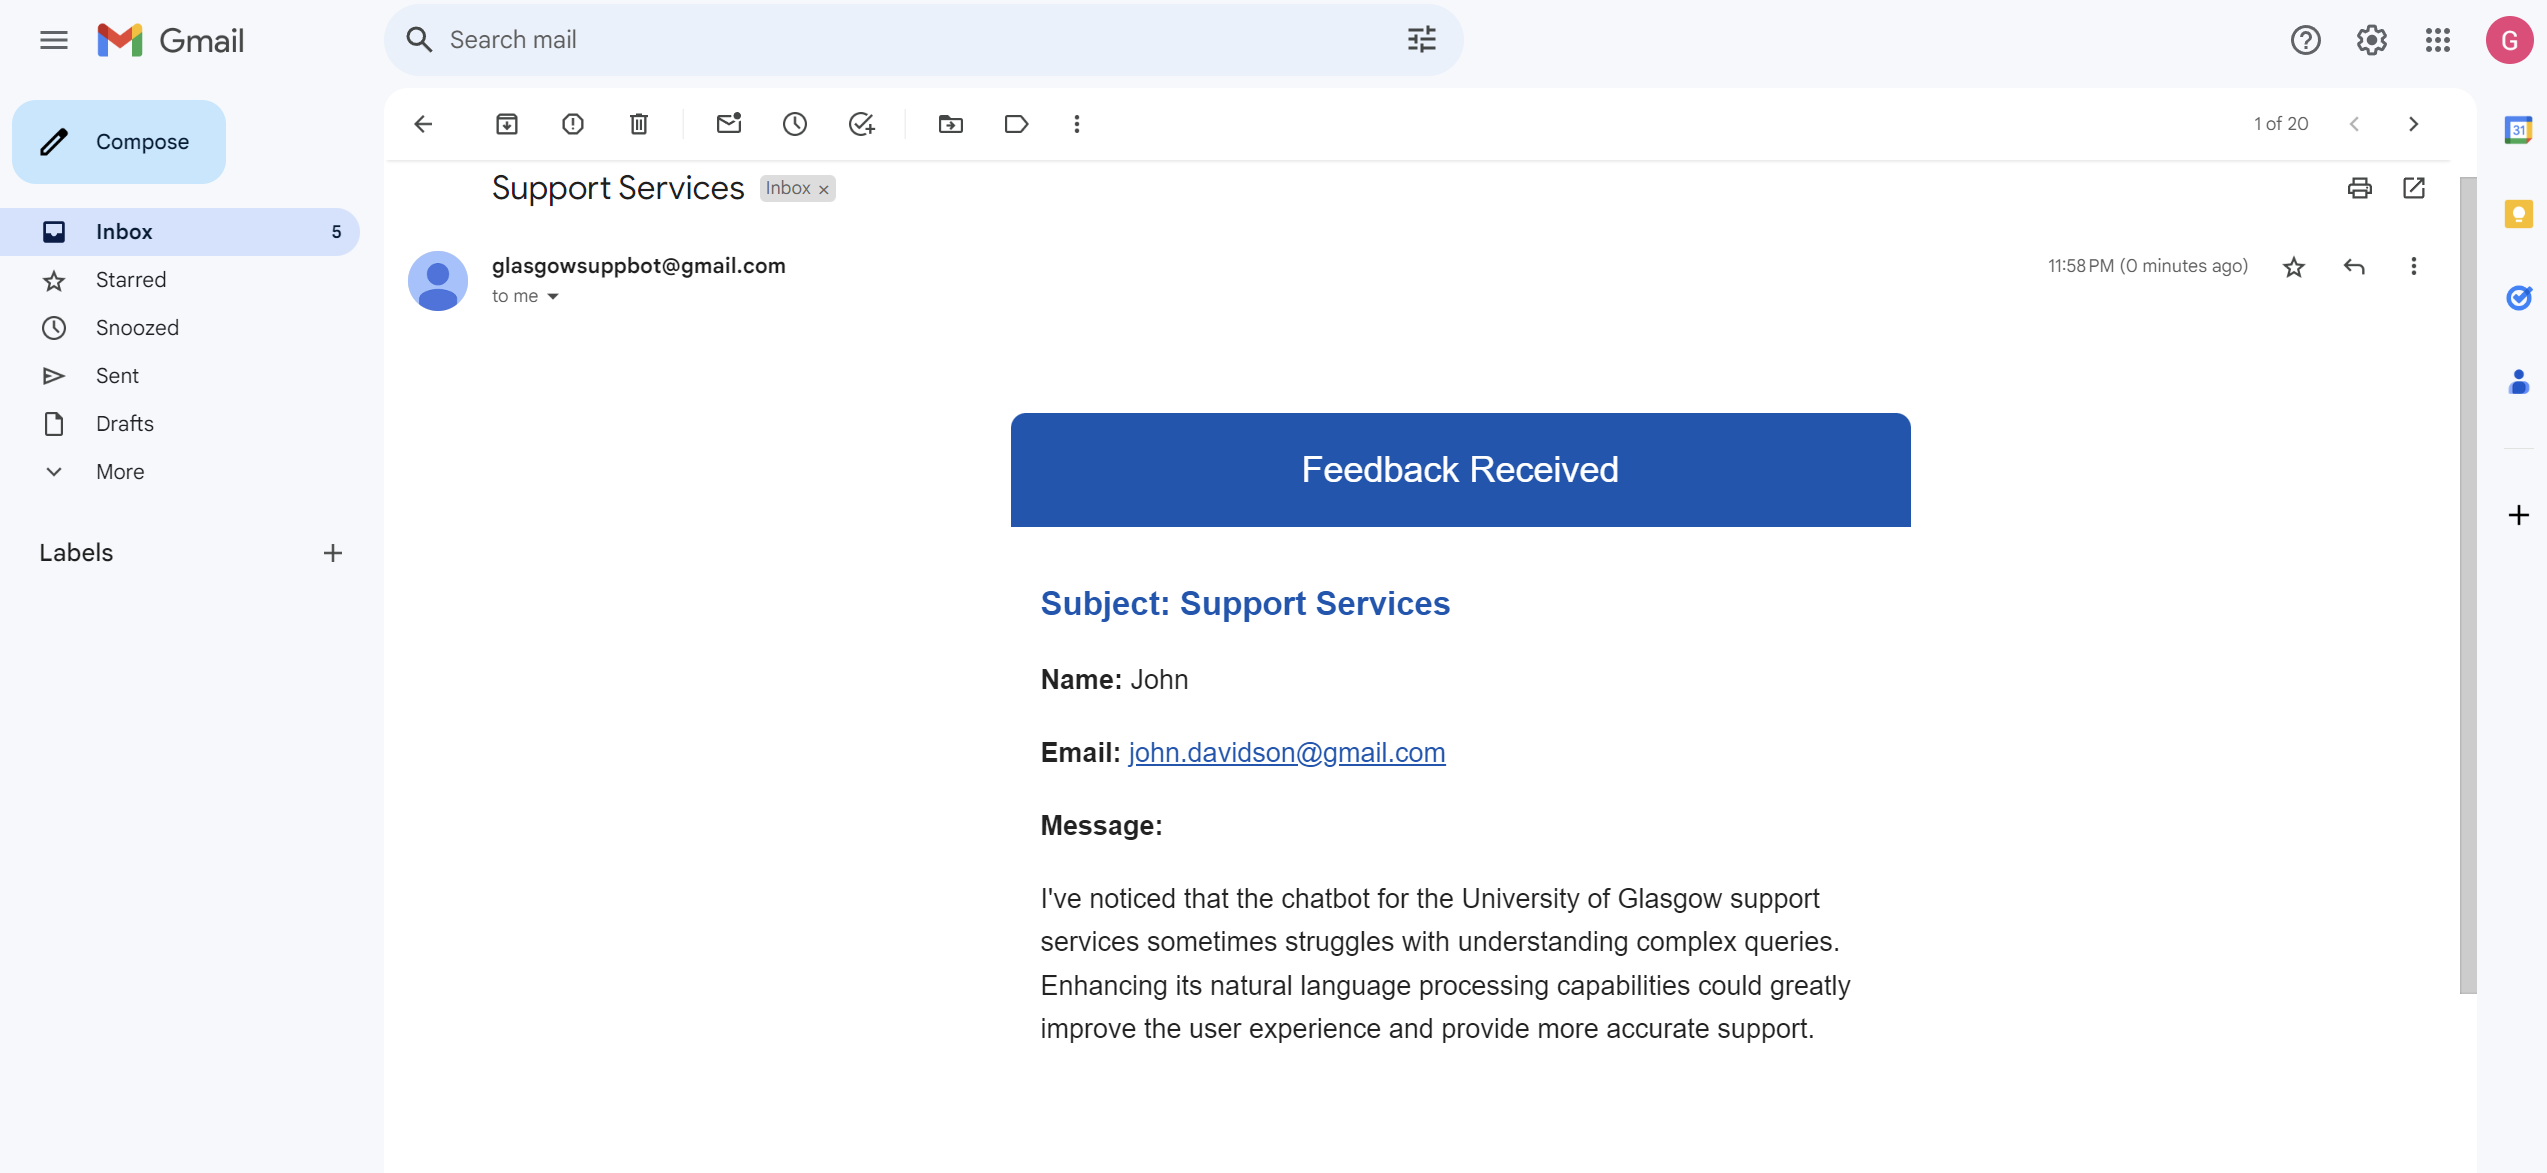
\includegraphics[height=1.65in]{images/emailfeedbackexample.png} % Ensure the height matches the other image
    \caption{Feedback Email Example}
    \label{fig:feedback_email_example}
  \end{subfigure}
\end{figure}



Once the feedback form is submitted, the data is encapsulated within a JSON payload and transmitted to the Flask back-end via an asynchronous POST request to the \textbf{/send-email} endpoint. Upon receiving the request, the back-end extracts the feedback details from the JSON payload. Using the extracted feedback details, the back-end dynamically generates an HTML email. This email is structured to highlight the feedback content clearly, making it easily interpretable by the support team. The construction of the email leverages the \textbf{email.mime.multipart.MIMEMultipart} and \textbf{email.mime.text.MIMEText} modules to create a multipart email with HTML content, ensuring that the feedback is presented in a reader-friendly format. Listing \ref{sendFeedback Function} presents the sendFeedback function that exists in the front-end. Additionally, it shows the \textbf{/send-email} endpoint, which is located on line 7.

\begin{lstlisting}[language=Python, caption={sendFeedback Function}, label={sendFeedback Function}]
const sendFeedback = async (event) => {
  event.preventDefault();
  if (!validateForm()) return;
  const feedbackData = { subject, name, email, message };

  try {
    const response = await fetch(`${process.env.REACT_APP_API_URL}/send-email`, {
      method: 'POST',
      headers: { 'Content-Type': 'application/json' },
      body: JSON.stringify(feedbackData),
    });
    
    const data = await response.json();
    if (data.success) {
      alert('Feedback sent! Thank you.');
      // Reset form state here
      setSubject(initialSubject);
      setName(initialName);
      setEmail(initialEmail);
      setMessage(initialMessage);
    } else {
      throw new Error(data.message || 'Failed to send feedback');
    }
  } catch (error) {
    console.error('Error sending feedback:', error);
    alert('An error occurred while sending feedback. Please try again.');
  }
};
\end{lstlisting}


The most technical aspect of this system is its integration with the Gmail API for sending the constructed email. This process involves authenticating with the Gmail API using OAuth 2.0 credentials, specifically through the use of refresh tokens to maintain a secure connection without requiring repeated user authorization. The Credentials object from \textbf{google.oauth2.credentials} is instantiated with the necessary OAuth 2.0 details, including the refresh token, client ID, and client secret—all of which are securely stored and accessed via environment variables loaded with \textbf{load\_dotenv()}. Upon refreshing these credentials to ensure a valid access token, the \textbf{googleapiclient.discovery.build} function creates a service object for the Gmail API, through which the email message, now encoded in base64 for compliance with email standards, is sent to the designated support email address, which is \textbf{glasgowsuppbotfeedback@gmail.com}. The only constraint to using OAuth is that the application is currently in test mode, not in production, which means that the refresh token will expire after 7 days; it is not designed for long-term use. However, it is entirely feasible to implement a long-lived refresh token if this web application were to be deployed for practical use.

\begin{lstlisting}[language=Python, caption={OAuth 2.0 \& Gmail API}]
def send_email(subject, name, email, message_text):
    CLIENT_ID = os.environ['CLIENT_ID']
    CLIENT_SECRET = os.environ['CLIENT_SECRET']
    REFRESH_TOKEN = os.environ['REFRESH_TOKEN']

    credentials = Credentials(
        None,  # Access token set to None, will use refresh token for access
        refresh_token=REFRESH_TOKEN,
        client_id=CLIENT_ID,
        client_secret=CLIENT_SECRET,
        token_uri='https://oauth2.googleapis.com/token',
        scopes=['https://mail.google.com']
    )

    credentials.refresh(Request())

    service = build('gmail', 'v1', credentials=credentials)
    message = create_message("glasgowsuppbott@gmail.com", "glasgowsuppbfeedback@gmail.com", subject, message_text)
    service.users().messages().send(userId="me", body=message).execute()
\end{lstlisting}

\section{Exporting Chat Histories}

Exporting chat histories is a feature that allows users to save and revisit their conversations for future reference. The technological implementation of this function is particularly interesting, as it includes both front-end logic for export generation and file download processing.

In \textbf{App.js}, the function \textbf{exportMessagesToTxt} is responsible for compiling the user's chat history into a text format. This involves iterating over the stored active chat messages, formatting them appropriately, and then constructing a Blob object that encapsulates the chat data. A URL is created from this Blob, and a download link is dynamically generated and triggered within the user interface, enabling the user to download their chat history as a \textbf{.txt} file. Please refer to \ref{Export Chat Messages to Text File.} to see how this was implemented.

\begin{lstlisting}[language=Python, caption={Export Chat Messages to Text File.}, label={Export Chat Messages to Text File.}]
const exportMessagesToTxt = () => {
    if (!activeChat || !activeChat.messages || activeChat.messages.length === 0) {
        alert("No messages to export.");
        return;
    }

    const chatContent = activeChat.messages.map(message => {
        // Assuming `sender` distinguishes between 'user' and 'ai'
        const senderPrefix = message.sender === 'user' ? 'User' : 'AI';
        return `${senderPrefix}: ${message.text}\n`;
    }).join('\n');
    
    const blob = new Blob([chatContent], { type: 'text/plain;charset=utf-8' });
    const url = URL.createObjectURL(blob);
    const link = document.createElement('a');
    link.href = url;
    link.download = `chat-history-${new Date().toISOString()}.txt`;
    document.body.appendChild(link);
    link.click();
    document.body.removeChild(link);
};
\end{lstlisting}

\section{Deployment}


To evaluate usability, the web app was set up so users could easily access it by clicking on a website link, avoiding the cumbersome process of installing files from GitHub. The back-end was deployed using Render and the front-end using Vercel.

\textbf{\cite{vercel}} is a cloud platform for static sites and serverless functions that makes it easy to deploy, scale, and secure web applications. It is particularly favored for projects built with React and other JavaScript frameworks, just like GlasgowSupportBot's front-end. Vercel stands out for its simplicity in deployment, and built-in CI/CD, which makes it an ideal choice for deploying the user interface of the web app. 

\textbf{\cite{render}}, on the other hand, is a cloud service that provides a unified platform to build and run all types of apps and websites with free SSL, private networks, and auto deploys from Git. The back-end of GlasgowSupportBot, built with Flask, benefits from Render's simplicity, and the ability to handle various back-end tasks without much overhead. The deployment process for GlasgowSupportbot is highly automated, with changes to the repository automatically triggering deployments to Vercel and Render, thanks to their built-in CI/CD capabilities.

Security is critical, especially when working with user data and integrating with third-party services. That is why sensitive keys like \textbf{CLIENT\_ID}, \textbf{CLIENT\_SECRET}, \textbf{OPENAI\_API\_KEY}, and \textbf{REFRESH\_TOKEN} are saved in Render's environment variables. These keys are required for secure authentication and interaction with Gmail and OpenAI APIs, and storing them in environment variables keeps them from being exposed in the codebase.

Similarly, on the Vercel side, environment variables like \textbf{REACT\_APP\_API\_URL} and \textbf{REACT\_APP\_ENCRYPT\_SECRET\_KEY} are used. The \textbf{REACT\_APP\_API\_URL} variable points to the back-end deployed on Render, facilitating the connection between the front-end and back-end. This setup ensures that the front-end can dynamically interact with the back-end, whether during development or in production. Specifically, \textbf{.env.local} contains \textbf{REACT\_APP\_API\_URL=http://localhost:5000} for local development, and \textbf{.env.production} contains \textbf{REACT\_APP\_API\_URL=https://glasgowsupportbot.onrender.com} for the production environment.

A challenge encountered was that the back-end would spin down after 15 minutes of inactivity in the free version of Render, leading to delays in handling queries. This was solved by sending frequent signals to the server using \textbf{UptimeRobot} to keep it from spinning down, ensuring that GlasgowSupportBot remains responsive and ready to assist users with no delays.

\section{Video Presentation}
The following link shows a demo of the features of GlasgowSupportBot implemented. You will be redirected to a Google Drive link when you click the link, you have to download the video to view it if it does not show.
Please access the demo using the following link: \href{https://drive.google.com/file/d/1ENyZklw4Tr3q2ZPeKW_s2tfDCbhWVlvJ/view?usp=drive_link}{\textbf{Video Demo Link}}.

%==================================================================================================================================
\chapter{Evaluation} 

This section delves into the evaluation of the GlasgowSupportBot project, focusing on two main assessment criteria: unit testing and user evaluation. The unit testing process is documented in tables that list the features tested, their pass or fail status, and the coverage of the code tested. Additionally, this chapter covers the methods used for evaluation, the outcomes of the process, and any limitations encountered during the assessment.

\section{Unit Testing}

In this section, unit tests were developed to verify the web application's performance and ensure its functionality aligned with expectations. Furthermore, these tests served to validate the correctness of the code implemented for GlasgowSupportBot. Both the front-end and back-end tests are directly integrated with GitHub's CI/CD automated testing workflows, ensuring that every push to the repository triggers the comprehensive suite of tests. The testing covers most functionalities across both the back-end and front-end components. Tables listing 28 different tests were created, including 13 for the back-end and 15 for the front-end. They are aimed at examining the internal workings of the code. Additionally, five extra user interaction tests were included for users to experiment within the GlasgowSupportbot. The table \ref{table:Sample Tests} below shows a sample of the test cases developed. It details various tests along with their descriptions and actual results, indicating whether each test passed or failed. The complete set of tests can be found in the Appendices, section \ref{Unit Testing}.

\begin{table}[htbp]
\centering
\renewcommand{\arraystretch}{1} % Adds more vertical space in the cells
\begin{tabular}{
    |>{\centering\arraybackslash}p{2cm}
    |>{\centering\arraybackslash}p{2cm}
    |p{6.5cm}
    |>{\centering\arraybackslash}p{2cm}|}
\hline
\rowcolor{HeaderColor}Type & Test Name & Description & Actual Result \\
\hline
\rowcolor{RowColor}Frontend & Chat History Render & Ensures the ChatHistory component properly renders with initial UI elements. & Passed \\
\hline
Backend & Environment Variables Load & Checks loading of all required environment variables for app configuration. & Passed \\
\hline
\rowcolor{RowColor}Frontend & Message Links Clickable & Validates that links within chat messages are interactive and clickable. & Passed \\
\hline
Backend & Send Email Functionality & Tests the complete functionality of sending an email, including service call chains and response handling. & Passed \\
\hline
\rowcolor{RowColor}Frontend & InputBox Typing State & Checks whether the InputBox disables the 'Send' button when the AI is 'typing,' simulating real-world async operations. & Passed \\
\hline
Backend & Query Database Success & Validates database querying capabilities, ensuring relevant search results return expected responses. & Passed \\
\hline
\end{tabular}
\caption{Selection of Frontend and Backend Unit Tests}
\label{table:Sample Tests}
\end{table}


For the back-end, we created a set of unit tests using Python's \textbf{pytest} framework, as well as mocking utilities like \textbf{patch} and \textbf{MagicMock}, to simulate the behavior of external dependencies without involving any data manipulation or network calls. This method ensured that our tests ran independently, focusing on the logic contained within our Flask application's endpoints and utility functions.
On the front-end, we leveraged \textbf{@testing-library/react} for React component testing, ensuring UI elements behaved as expected in response to user interactions and data changes. Mocking was extensively used here as well, particularly for network requests (using \textbf{jest.mock}). An example of a test is shown below in Figure \ref{Test Example.}.

\begin{figure}[h!]
  \centering
  \begin{adjustbox}{center,max height=0.2\textheight, max width=\linewidth}
    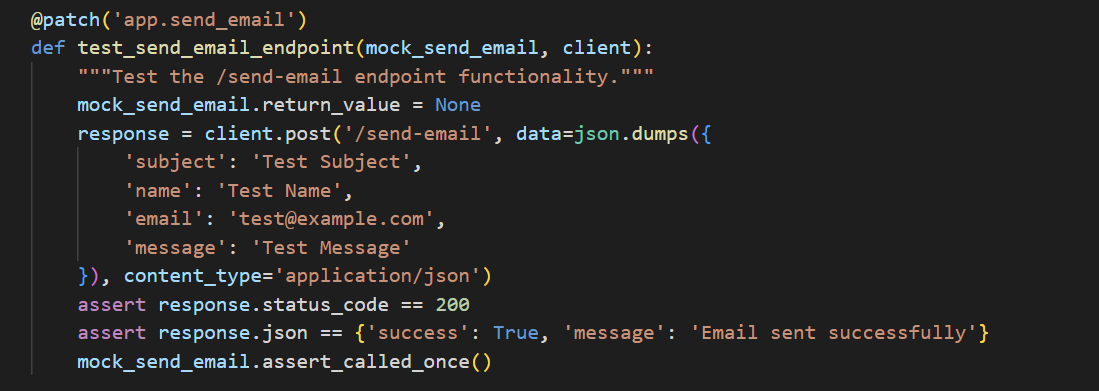
\includegraphics{images/testexample.png}
  \end{adjustbox}
  \caption{Test Example.}
  \label{Test Example.}
\end{figure}


All 28 tests in both the back-end and front-end have passed. The code coverage report provides a measure of how comprehensively the current test cases evaluate the codebase. Using a coverage tool integrated within Visual Studio Code, we have quantified the percentage of the code that has been tested across various files in the application, as demonstrated in figures \ref{fig:backendcodecoverage} and \ref{fig:frontendcodecoverage}. Figure \ref{fig:frontendcodecoverage} represents the front-end and figure \ref{fig:backendcodecoverage} represents the back-end.

\begin{figure}[ht]
  \centering
  % First Image
  \begin{adjustbox}{valign=t}
    \begin{subfigure}[b]{0.49\textwidth}
      \centering
      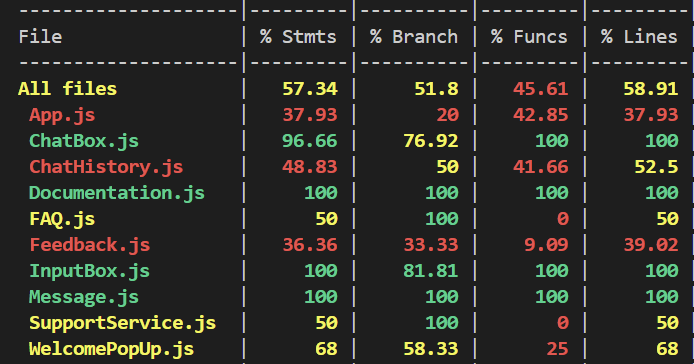
\includegraphics[height=3.5cm]{images/frontendcoverage.png}
      \caption{Frontend Code Coverage.}
      \label{fig:frontendcodecoverage}
    \end{subfigure}
  \end{adjustbox}
  \hfill % Space between the two images
  % Second Image
  \begin{adjustbox}{valign=t}
    \begin{subfigure}[b]{0.49\textwidth}
      \centering
      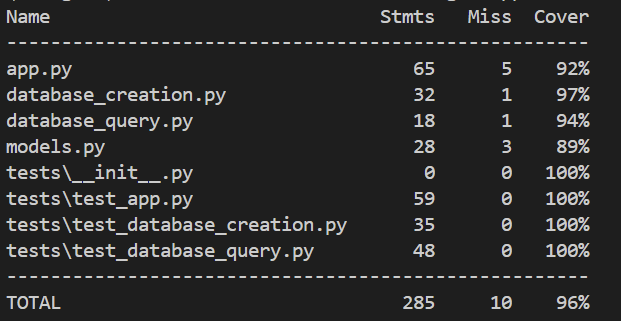
\includegraphics[height=3.5cm]{images/backendcoverage.png}
      \caption{Backend Code Coverage.}
      \label{fig:backendcodecoverage}
    \end{subfigure}
  \end{adjustbox}
\end{figure}




\section{User Evaluation}
The GlasgowSupport website is intended to be used not only in Glasgow but also worldwide. As a result, it was possible to include evaluators from all around the world in the assessment process. The evaluation adhered to the School of Computing Science ethical checklist in Appendices, Section \ref{Ethical Checklist}. The compressed folder contains a comprehensive collection of materials gathered from the survey, including images from the responses, an excel sheet summarizing the data, audio recordings of the interviews, and their corresponding transcripts for detailed analysis.

\subsection{Methodology}

A Google Form survey was developed as the principal method for gathering user feedback on GlasgowSupportBot, aiming to assess the usability and user experience of the chatbot. The URL link to GlasgowSupportBot was included in the survey. Participants were advised to use a computer or laptop to ensure consistency in response time and interaction quality. In the first section of the survey, users engaged with the chatbot by completing 5 tasks and answering 13 questions, designed to evaluate various facets of the bot's functionality, from how it handles specific queries to its ability to manage complex or unrelated questions. The second section employed the System Usability Scale (SUS) questionnaire, a reliable tool for measuring a system's usability with 10 questions. These questions addressed aspects of the user experience such as the system's ease of use, integration of functions, consistency, and the user's confidence in using the system. Answers from the SUS questionnaire were used to calculate an average SUS score, providing a quantitative measure of GlasgowSupportBot's usability.

\subsection{Analysis of Responses}
The analysis of participant responses from the survey will be detailed below.
The survey form, along with all the questions, is available in the Appendices, section \ref{Evaluation Survey}. Most of the participants adhered to the tasks they were given as it is evident from the responses given.

\textbf{Initiation of User Interaction}

For effective user engagement, the ease with which users can begin using the chatbot is vital. Notably, 60.9\% of participants reported that starting a conversation with GlasgowSupportBot was 'Very Easy', while 39.1\% rated it as 'Easy'. These numbers suggest that users can navigate the chatbot with ease and find its features clear when they first visit the website. In creating the chatbot, consideration was given to the users' experience with other intuitive platforms, including systems like ChatGPT. The aim was to ensure that the chatbot would be user-friendly and familiar to users right from the start.

\textbf{Informational Reliability}

The accuracy of GlasgowSupportBot's responses is important in building users' trust. Impressively, 100\% of participants rated the bot's information as either 'Very Accurate' or 'Accurate', highlighting its ability to deliver dependable support information consistently. The evaluation scenarios were varied, including instances where users posed questions from different viewpoints, such as someone seeking mental health assistance. The bot demonstrated remarkable adaptability, accurately interpreting the context and adjusting its responses based on the specific way questions were asked. Moreover, the bot's ability to comprehend queries correctly, even in the presence of minor spelling errors, further emphasizes its reliability. 

\textbf{Concurrent Query Management}

Users recognized GlasgowSupportBot's capability in managing several queries within a single interaction, with 52.2\% of participants rating this feature as 'Poorly' and 26.1\% as 'Neutral'. The majority of feedback indicates that the performance in this area did not meet user expectations. Having the ability to effectively manage multiple queries in one interaction is crucial for a chatbot's functionality. Despite several attempts to enhance this feature, challenges persisted, and it has not yet reached the desired level of efficiency. Therefore, improving this aspect of the chatbot is considered a key area for future development.

\textbf{Preference for the Chatbot}

In the comparison between GlasgowSupportBot and the university's traditional website, a notable preference for the chatbot was observed, with 52.2\% of users showing a strong preference for the chatbot, while 30.4\% had no specific preference.

This preference was thoroughly evaluated through specific tasks designed to assess the chatbot's effectiveness against the website. One such task involved participants seeking particular information on the university's website, which was also available through the chatbot. Notably, in Task 2, users were directed to find information about "good cause categories" by both using the university's website and querying the chatbot. Subsequently, they were asked to rate which method was more effective based on their experience. This direct comparison method was employed to gauge the chatbot's ability to provide information compared to the conventional method of searching on the website.

Moreover, it's worth noting that while simple questions might be quickly answered through a standard internet search, the chatbot excels in delivering in-depth responses. For comprehensive answers that require more detailed information, GlasgowSupportBot is likely to outperform the conventional approach of searching online. 

\textbf{Additional Suggestions for Improvement}

In the feedback received, 11 out of the 23 participants offered valuable suggestions for improving GlasgowSupportBot. Among these suggestions, four key areas stand out,

\begin{enumerate}
    \item \textbf{Integration with University Systems:} A user expressed a wish for the chatbot to be linked with the university's login systems. Such a connection would make the chatbot more efficient by providing advice and support that directly relates to a student's own courses and administrative needs. This would make accessing personal and relevant university information easier and more direct.
    
    \item \textbf{Interactive Features:}  Introducing interactive elements, such as buttons for quick responses to common questions, was suggested to simplify and enhance user interactions. This would make using the chatbot quicker and more straightforward, especially for frequently asked questions, by reducing the amount of typing needed. 
    
    \item \textbf{Design Customizability:} There was a desire among users for options to customize the look of the chatbot, such as changing color themes or enabling a dark mode. Allowing users to adjust the chatbot’s appearance could improve their comfort and make the chatbot feel more personal, particularly for those who spend a lot of time interacting with it.

    \item  \textbf{Topic Exploration} A user expressed a need for an easier way to understand which questions they can ask, especially since the chatbot's support services are limited to specific areas. There's a call for improvements that would make it clearer for users to identify the scope of topics covered by the chatbot. By providing a more straightforward method, such as a list or a visual guide of potential questions or topics next to the chat interface, users could ask the chatbot more appropriately. 
\end{enumerate}


\subsection{Multiple Choice Questions - Quantitative Data}


To collect quantitative feedback information for evaluating the usability of GlasgowSupportBot, ten multiple-choice questions were used to generate the SUS score for each participant. These questions, discovered through a methodology detailed at \cite{questionproSystemUsability} include a mix of positive and negative questions, with participants responding on a five-point Likert scale ranging from Strongly Disagree to Strongly Agree. Positive questions are placed at odd numbers, while negative questions are even numbered. To compute the SUS score for each individual, one point is subtracted from the score of each of the positive questions. For negative questions, the participant's response is subtracted from 5. These scores are subsequently summed and multiplied by 2.5 to obtain the overall SUS score which is expressed as a percentage ranging from 0 to 100. According to \cite{questionproSystemUsability}, a perfect score of 100\% indicates flawless usability. The average benchmark is 68\%. Scores over 70\% indicate good usability, implying an excellent level of user interface efficiency. Scores below 50\%, on the other hand, show an urgent need for usability improvements, pointing to severe flaws that may impede user satisfaction. The SUS Questions used can be found in the Appendices in section \ref{Evaluation Survey} in survey figure \ref{fig: Survey Page 4}. The SUS scores for all 23 participants can be found in Appendices in section \ref{System Usability Student Results}.


\begin{table}[htbp]
  \centering
  \begin{tabular}{cccccccccccccc}
    \toprule
    Participant & Q1 & Q2 & Q3 & Q4 & Q5 & Q6 & Q7 & Q8 & Q9 & Q10 & Total & SUS Score \\
    \midrule
    Student 1 & 5 & 2 & 5 & 1 & 4 & 2 & 5 & 1 & 5 & 2 & 36 & 90.0 \\
    Student 2 & 4 & 1 & 5 & 1 & 4 & 1 & 5 & 1 & 5 & 1 & 38 & 95.0 \\
    Student 3 & 4 & 2 & 4 & 2 & 4 & 1 & 5 & 1 & 5 & 2 & 34 & 85.0 \\
    Student 4 & 3 & 1 & 5 & 1 & 4 & 2 & 5 & 1 & 5 & 2 & 35 & 87.5 \\
    Student 5 & 3 & 1 & 5 & 1 & 4 & 2 & 5 & 2 & 5 & 1 & 35 & 87.5 \\
    Student 6 & 3 & 2 & 4 & 2 & 4 & 2 & 4 & 3 & 5 & 2 & 29 & 72.5 \\
    Student 7 & 5 & 1 & 5 & 2 & 4 & 2 & 4 & 2 & 4 & 1 & 34 & 85.0 \\
    Student 8 & 4 & 2 & 5 & 1 & 5 & 1 & 5 & 2 & 4 & 1 & 36 & 90.0 \\
    \bottomrule
  \end{tabular}
    \caption{Participants SUS Scores.}
    \label{table: Participants SUS Scores.}
\end{table}

Table \ref{table: Participants SUS Scores.} presents a sample of the System Usability Scale (SUS) scores. The average score of all participants is 88.5. This score suggests a high level of satisfaction with the website. It is worth noting, however, that four participants had SUS scores below 81, indicating that certain aspects of the website should be improved further.

\subsection{Open-Ended Questions - Qualitative Data}

The final section of the evaluation required participants to answer certain open-ended questions.
Participants were asked about their favorite and least favorite aspects of GlasgowSupportBot, as well as which features were most essential to them and suggestions for changes to the design.

\textbf{What People Like Least about GlasgowSupportBot}

Participants in the evaluation shared their concerns about GlasgowSupportBot, focusing particularly on the user interface and overall design. They found the layout too simplistic. Also, one of the participants mentioned a significant issue with the way text was displayed and the lack of clear differentiation between messages from the user and the bot, which complicated the reading and interaction process. Additionally, participants felt the bot struggled with follow-up questions, indicating that it often failed to recognize the context of the conversation, which resulted in unsatisfactory exchanges.

\textbf{What People Like Most about GlasgowSupportBot}

Participants praised GlasgowSupportBot, notably its efficiency and user-friendly interface, which allowed for simple access to information and services. The bot's ability to provide straight and precise responses was a standout feature, allowing users to swiftly get the specific information they required without unnecessary clarification. Its simple design was praised for being user-friendly, allowing even those with less technological knowledge to explore and interact with ease. Furthermore, the bot's wide range of meaningful support services received high praise; participants appreciated the ease of access to essential university support services, such as well-being and mental health, highlighting the bot's role in providing valuable guidance and support to the student body. Furthermore, the feature that allows chat exports was noted as very helpful. Also, the addition of clickable links in the responses was seen as useful.

\textbf{Recommended Improvements for GlasgowSupportBot}


Participants suggested a variety of improvements to enhance GlasgowSupportBot's functionality and user experience. One of the recommendations mentioned was the introduction of automatic greeting messages or prompts from the bot at the start of interactions. Even though \textbf{WelcomePopUp.js} was created to greet the user, participants still felt that having such a feature would make the initial engagement more inviting and straightforward. Additionally, one participant mentioned expanding the bot's knowledge base beyond just support services to include a wider range of information about Glasgow University. This expansion would significantly enrich the bot's utility, providing users with a more comprehensive resource for university-related inquiries. As mentioned before in section \ref{Support Services Information Retrieval}, this is entirely possible and easy to do.

A frequent request from the participants was to enhance the bot's AI to better manage follow-up questions. This would ensure conversations flow more smoothly and naturally. Finally, the introduction of structured responses, such as the use of bullet points, indentations, or spacing, was recommended to make the bot's answers easier to digest and understand. This approach would help organize information more clearly, improving readability and user satisfaction.

\textbf{Design Improvements}

Participants made several suggestions targeted at improving the user experience, with a particular interest in a more customizable interface. Among the interesting improvements recommended was the addition of a night mode option, which could make the screen easier on the eyes in low light. The feedback icon was also brought up during the interview; it seems that it needs to be clearer about what it does, so people understand its use straight away. Beyond functionality, there was a desire for a more bright and interesting interface. While the simplicity of the current design was much praised, adding more colors and visual components is suggested as an effective way to make the interface not only more visually appealing but also more engaging for users.


\section{Chapter Summary}

In this chapter, the unit testing and evaluation of GlasgowSupportBot was covered. The unit tests were designed to examine the internal workings of the code. 28 unit tests and 5 user interaction tests were created. For more coverage, additional tests can be developed in the future. For the evaluation process, a combination of open-ended questions, the System Usability Scale, and a survey were employed. Among the 27 participants, with 23 participants responding to the survey and 4 participants to open-ended questions, the majority commended the application's features and user interface. They believe that GlasgowSupportBot can be used for the university if some key features are to be implemented in the future. 



%==================================================================================================================================
\chapter{Conclusion}   

This chapter will summarize all the chapters in the dissertation about the GlasgowSupportBot project. It will address the limitations that hindered the project's further development, as well as potential future improvements. The chapter will conclude with a reflection on the methods and procedures used in the project.

\section{Summary}

GlasgowSupportBot is a web application that offers detailed information on support services at the University of Glasgow, including disability support, mental health resources, and international student assistance. GlasgowSupportBot was created to allow anyone to swiftly inquire about support services directly through the bot, eliminating the necessity to browse through websites. It was carefully designed and deployed to make it available to students around the world especially Glasgow University students who may benefit from its services in the future. To determine the system's effectiveness and usability, two main evaluation methodologies were used: unit testing and user evaluation. Unit testing was carried out to evaluate the bot's functionality, guaranteeing that every feature performed as intended. This testing primarily targeted the internal code with a focus on ensuring the bot delivered precise and reliable responses. Regarding user evaluation, participants took part in a survey that included specific tasks, followed by the completion of the System Usability Scale (SUS) for quantitative data and open-ended questions for qualitative insights. This method allowed for a comprehensive evaluation of the user experience as participants engaged with the chatbot, exploring its features and navigating through the information on support services. The feedback received was impressive, with many users praising the ease of use and the benefits of having a consolidated source for support service information. The study of quantitative data revealed impressive usability scores, indicating a high level of user satisfaction. Furthermore, participants reported a significant desire to continue using the bot, particularly if it was updated with new features and services. To view the deployed web application, please visit GlasgowSupportBot at \url{https://glasgowsupportbot.vercel.app/}. To build and run GlasgowSupportBot locally, source code files comprised of back-end and front-end are located in the root directory inside the compressed folder. Instructions on how to build, set up the environment, and install
required dependencies are in README.md. A 9-page user guide, titled UserGuide.pdf is located in the UserGuide folder. It contains step-by-step guidance on using the system
and all screenshots of GlasgowSupportBot.

\section{Future Work}

For the future development of GlasgowSupportBot, feedback from users has highlighted several areas where improvements can make the bot more effective and easier to use. Users have pointed out that the design of the bot could be more engaging. Currently, the design is very basic, and it's hard for users to tell apart messages from the bot and messages they type themselves. This feedback suggests a need for a more visually appealing design that differentiates between user and bot messages.

Additionally, users have found that the bot sometimes struggles to understand follow-up questions. This means the bot doesn't always recognize when a user is continuing a conversation on a previous topic, leading to confusion or unsatisfactory answers. Addressing this issue by making the bot smarter in recognizing context and follow-up questions can significantly improve the conversation flow, making interactions feel more natural.

Enhancing the bot's knowledge is another critical area of future work. Currently, the bot provides support on a range of topics, but users have expressed interest in having access to a wider variety of information about Glasgow University. By expanding the topics the bot can cover, it can become an even more valuable resource for users, offering answers to a broader range of questions about the university.

Improvements in how the bot presents information could also greatly benefit users. Suggestions include organizing the bot's responses better and using bullet points or different formatting to make information easier to read and understand. This approach allows users to rapidly locate the information they need without having to go through enormous amounts of text.

From a technical perspective, introducing a limit on the number of queries a user can ask could help manage costs, especially considering the expenses associated with using  OpenAI. Another important limitation to focus on is Render. Currently, the bot's backend is hosted on the free version of Render, which automatically shuts down the server after 15 minutes of inactivity. By upgrading to a more continuous service, the bot could respond more quickly to users at any time, making it more reliable and pleasant to use.

Moreover, moving from a testing phase to a fully operational production phase is crucial. In the test phase, the bot uses an OAuth refresh token to securely send feedback to the developers. However, these tokens expire every 7 days. By shifting to a production environment, we can use tokens that last much longer, which means less maintenance and a more stable feedback service for users.
\section{Final Reflection}

In concluding my dissertation, I reflect on the journey undertaken with the GlasgowSupportBot project,  which proved both challenging and rewarding. This project was a practical application of the software engineering ideas I learned at the University of Glasgow, helping me to bridge the gap between academic knowledge and real-world application. The GlasgowSupportBot project was instrumental in my professional and personal growth, pushing the boundaries of my technical knowledge and skill set. Creating GlasgowSupportBot with technologies previously unfamiliar to me has greatly enhanced my programming skills. Learning how to manage time was an important element of this project. When tasked with executing a large-scale project, I learned how to break down difficult work into smaller steps and use time management tools successfully. This method improved my workflow and also gave me a feeling of discipline and organization in my work habits. The GlasgowSupportBot's success was due in large part to research. Learning how to conduct an extensive background study was very important in establishing a solid foundation for the project. Another key aspect of my learning experience was evaluating software. Gaining insight into how systems are used while also collecting feedback were critical steps in finding areas for improvement. This experience helped me understand the importance of user feedback in the software development process.

In retrospect, the GlasgowSupportBot project was a transforming experience. It has not only increased my technical skills and knowledge, but also improved my research, time management, and evaluation abilities. These lessons will surely be valuable in my future endeavors in software engineering.


%===============================================================================================================
%==================================================================================================================================
%  APPENDICES  

\begin{appendices}
\chapter{Ethical Checklist}
\label{Ethical Checklist}

\begin{figure}[h!]
  \centering
  \begin{adjustbox}{center,max height=0.8\textheight, max width=\linewidth}
    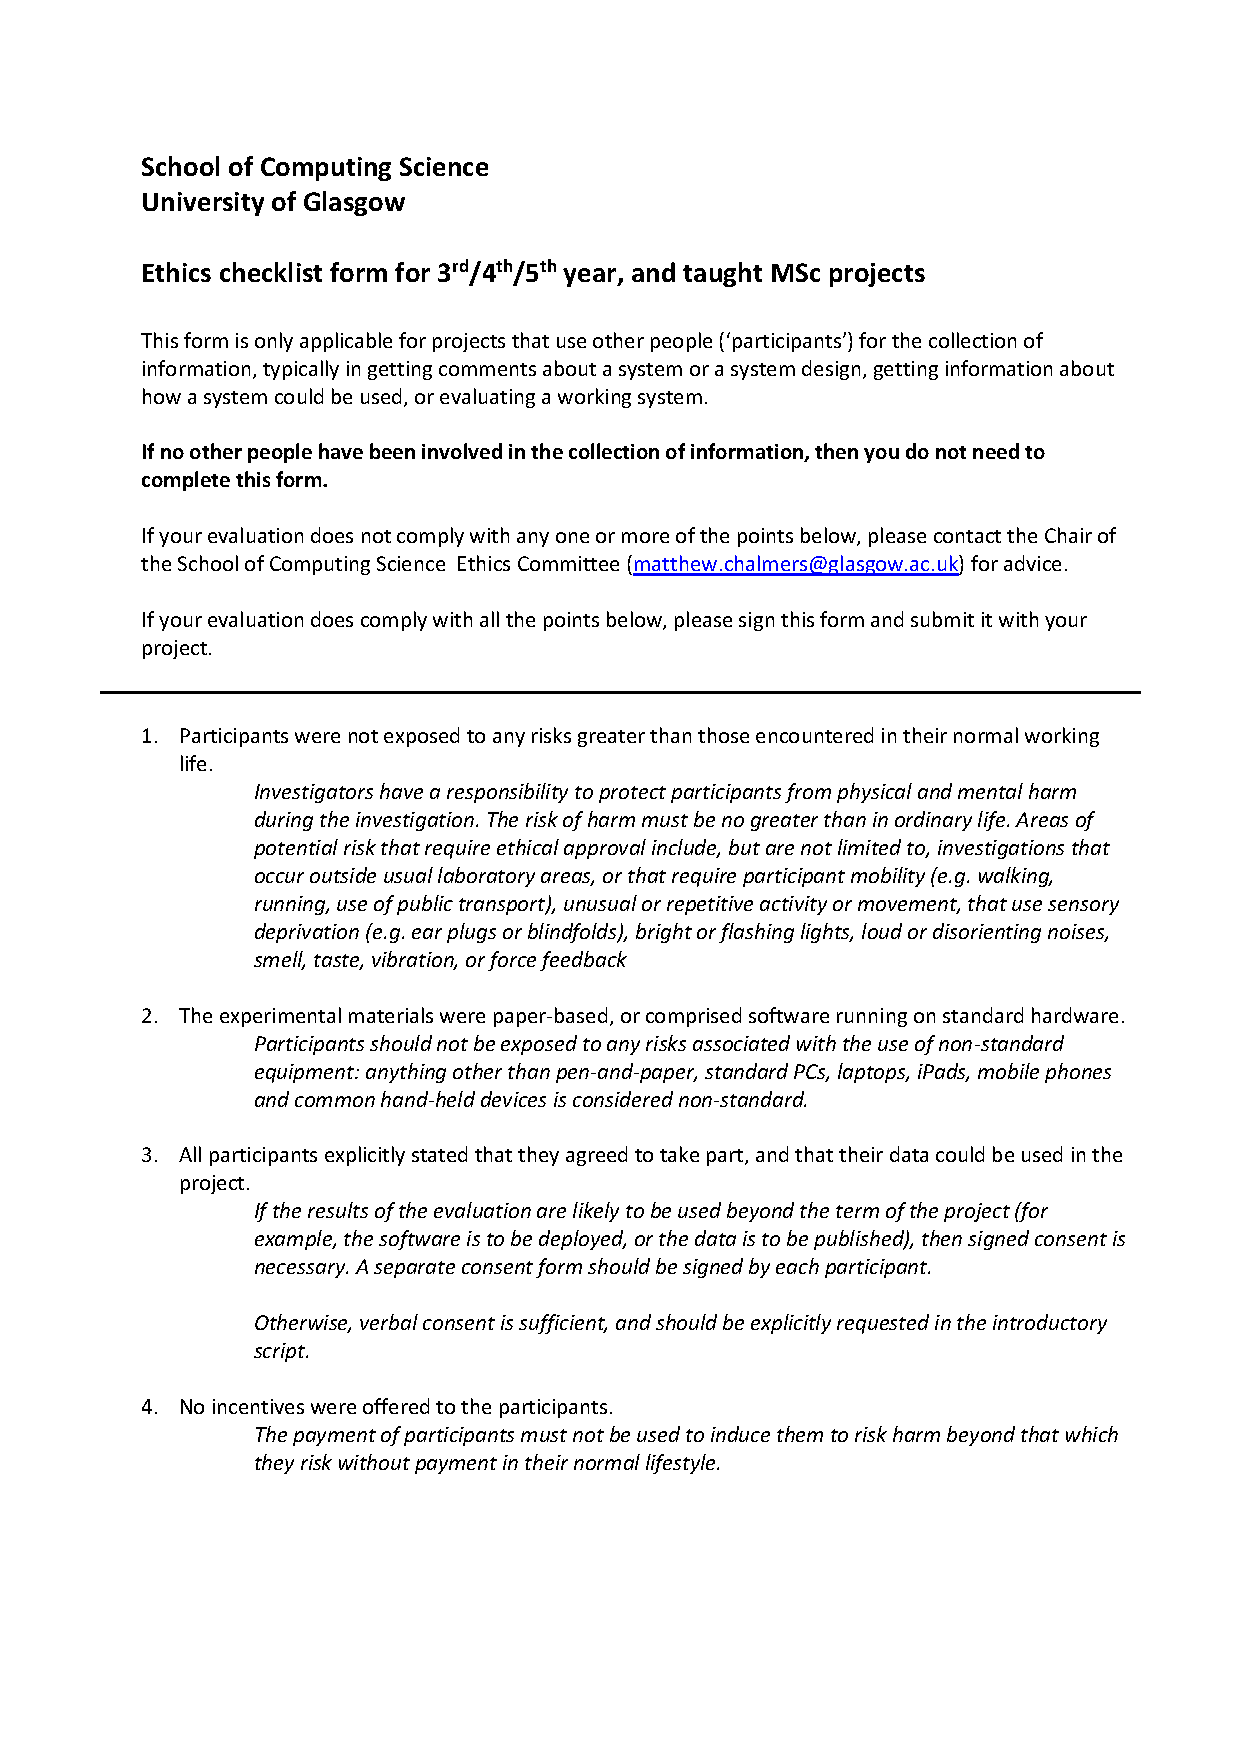
\includegraphics{images/Nader_Ethical_Checklist_1-1.pdf}
  \end{adjustbox}
\end{figure}

\begin{figure}[h!]
  \centering
  \begin{adjustbox}{center,max height=0.9\textheight, max width=\linewidth}
    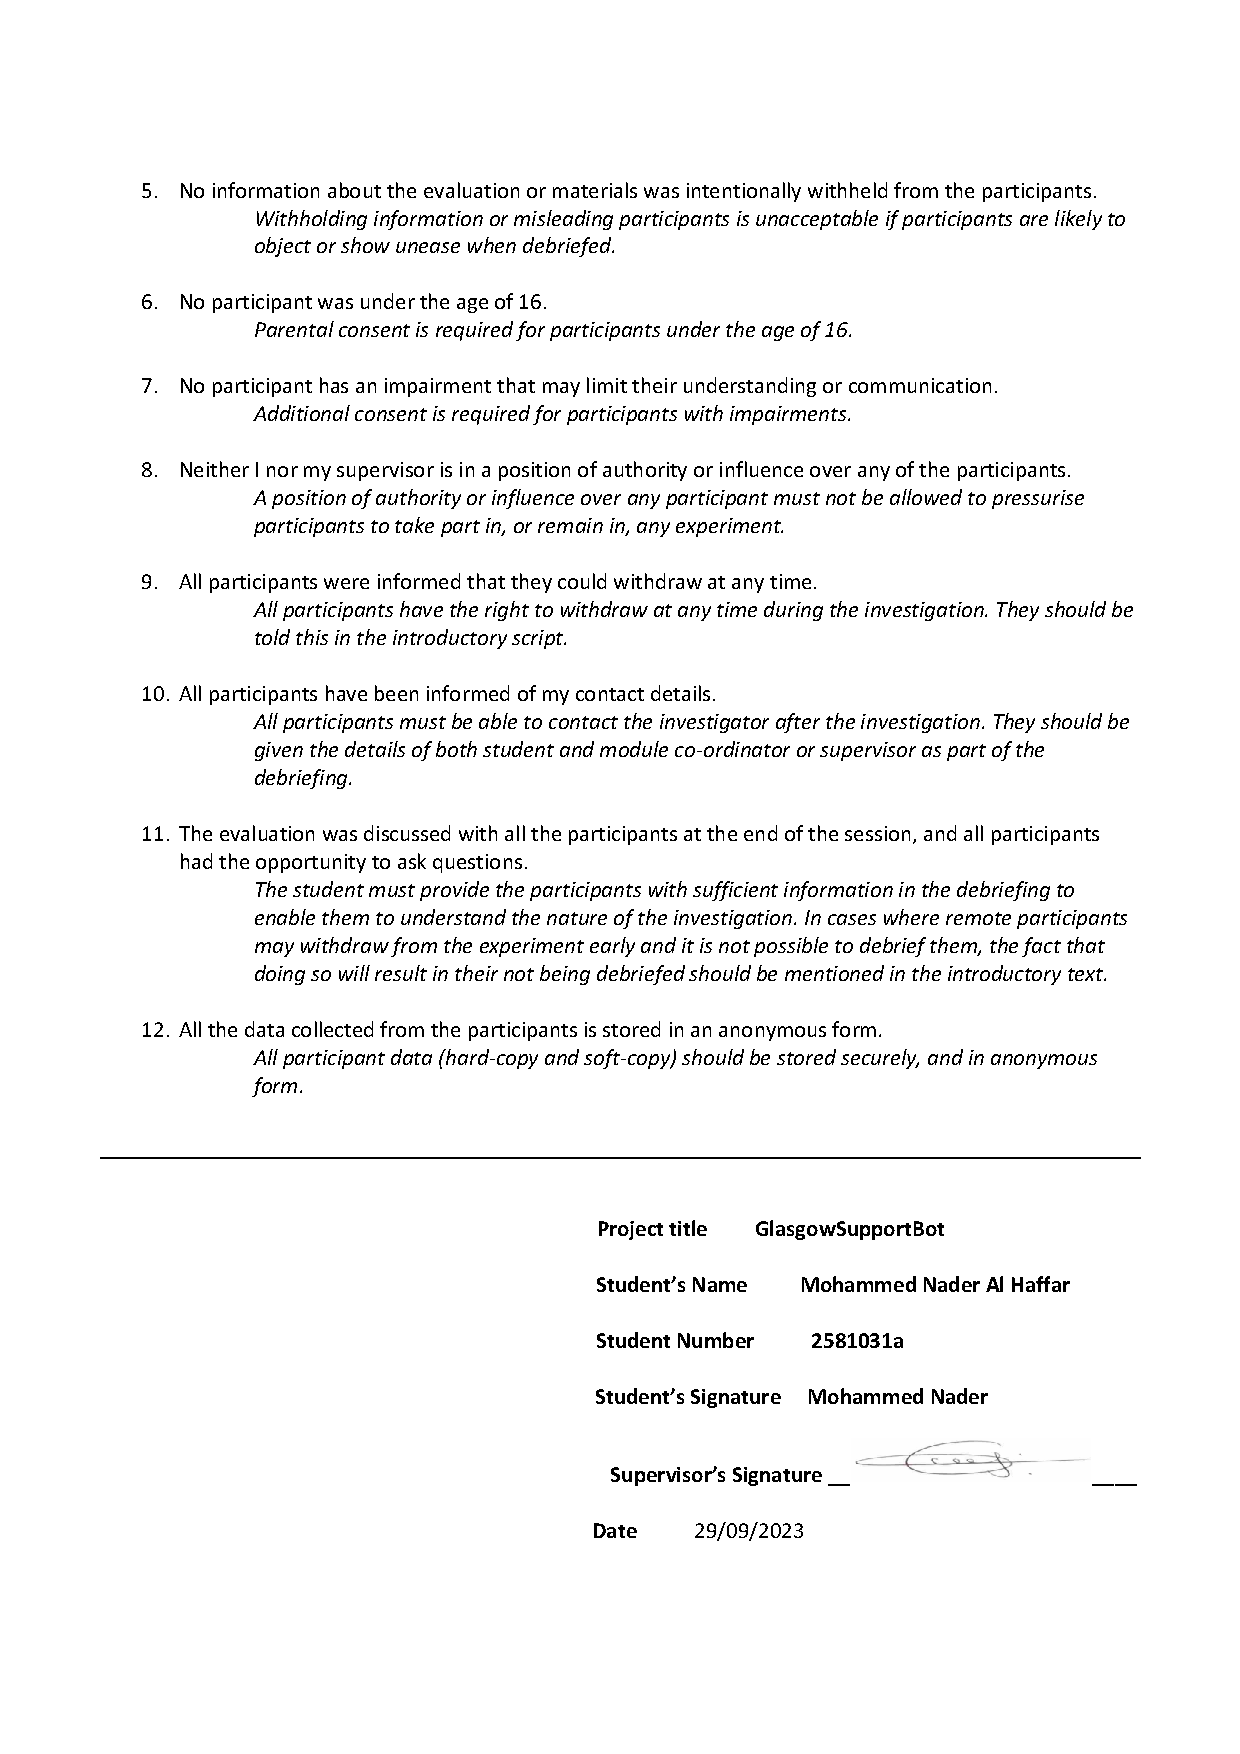
\includegraphics{images/Nader_Ethical_Checklist_2-end.pdf}
  \end{adjustbox}
\end{figure}


\chapter{User Personas}
\label{ch:User Personas}


\noindent\begin{minipage}{\linewidth}
    \centering
    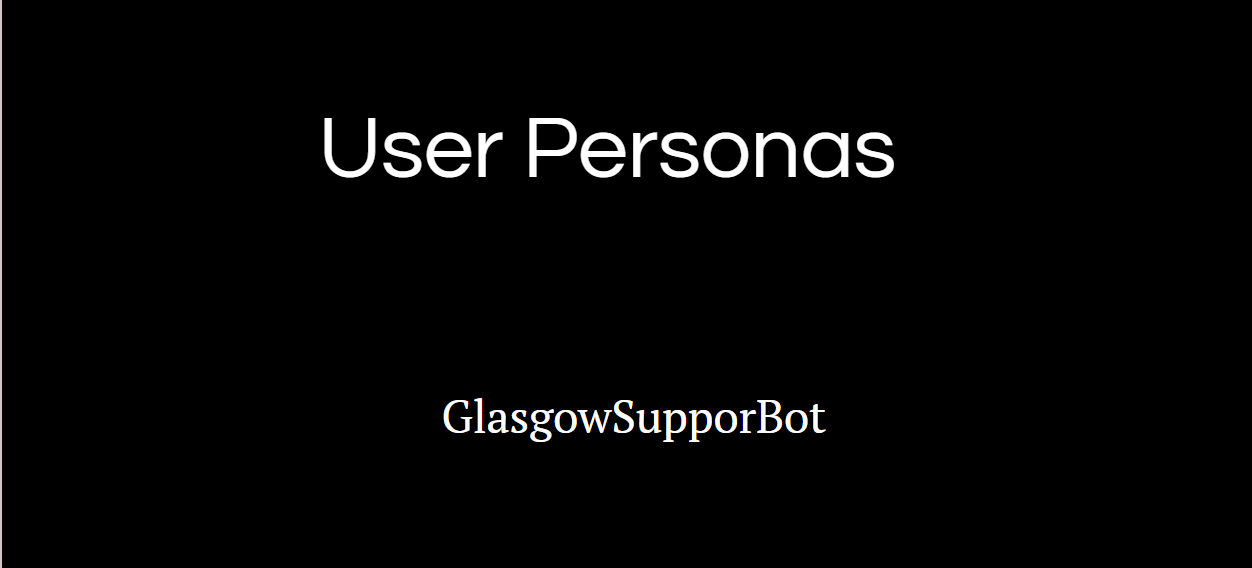
\includegraphics[width=\linewidth]{images/userpersonas.png}
\end{minipage}

\vspace{-10pt} 
\noindent\begin{minipage}{\linewidth}
    \centering
    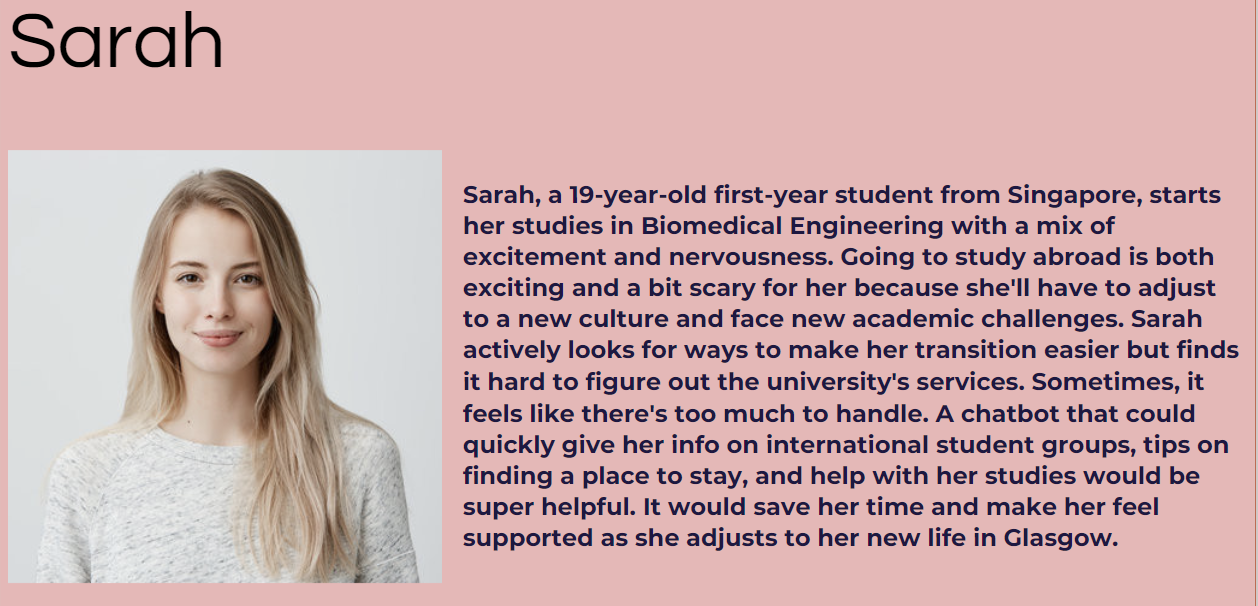
\includegraphics[width=\linewidth]{images/Sarah.png}
\end{minipage}

\vspace{-10pt} 

\noindent\begin{minipage}{\linewidth}
    \centering
    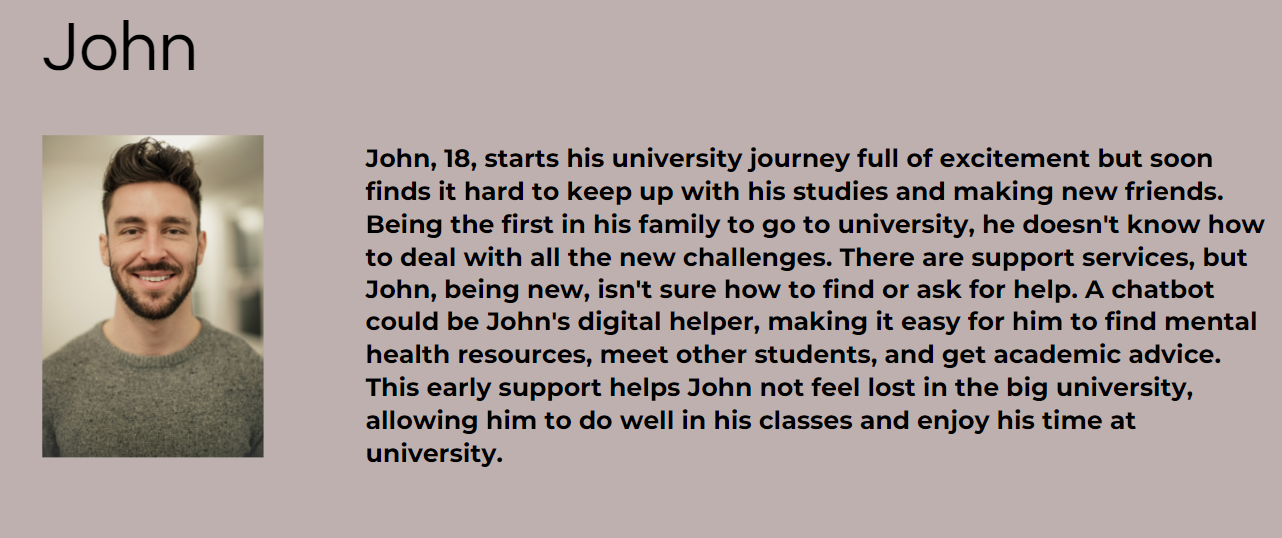
\includegraphics[width=\linewidth]{images/John.png}
\end{minipage}

\vspace{-10pt} 

\noindent\begin{minipage}{\linewidth}
    \centering
    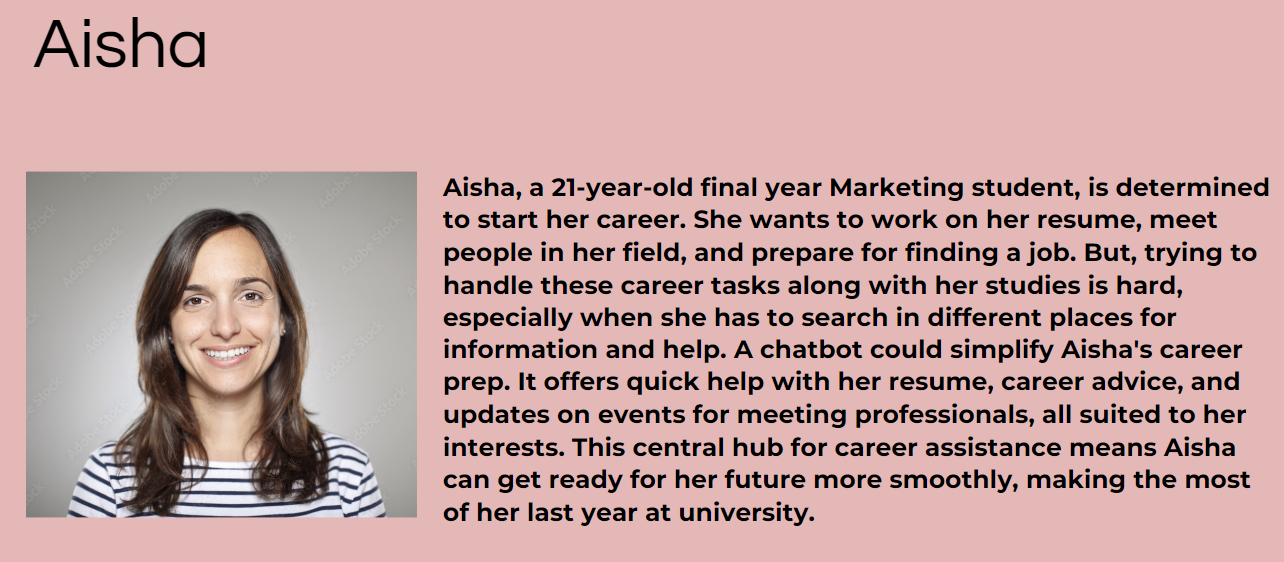
\includegraphics[width=\linewidth]{images/Aisha.png}
\end{minipage}

\vspace{-10pt} 

\noindent\begin{minipage}{\linewidth}
    \centering
    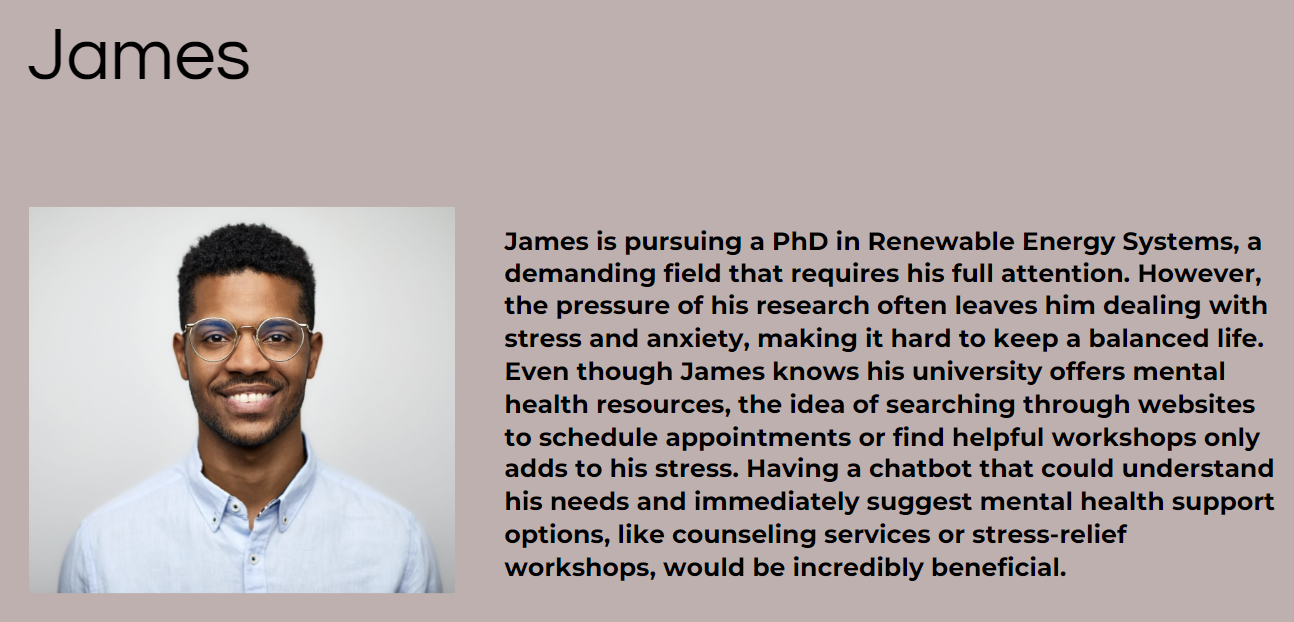
\includegraphics[width=\linewidth]{images/james.png}
\end{minipage}

\chapter{User Stories}
\label{ch:User Stories}


\section*{User Stories Structure}
\begin{itemize}
    \item[] {\large As a \textbf{[description of user]},}
    \item[] {\large I want \textbf{[functionality]},}
    \item[] {\large so that \textbf{[benefit]}.}
\end{itemize}

\section*{Support Services}
\begin{itemize}
    \item As a student with disabilities, \\I want to know how to register for support \\so that I can receive the necessary accommodations for my courses.
    \vspace{1em}
    \item As an international student, \\I want guidance on applying for a Student Visa outside the UK, \\so that I can ensure my application is successful and timely.
    \vspace{1em}
    \item As a student facing mental health challenges, \\I want to find out how to register for counseling services \\so that I can get the support I need as soon as possible.
    \vspace{1em}
    \item As a student who needs to make a Good Cause claim, \\I want to understand what evidence I need to provide \\so that my claim has the best chance of being accepted.
    \vspace{1em}
    \item As a student with a specific learning difficulty, \\I want information on the Disabled Students' Allowance (DSA) \\so that I can apply for financial support.
   
    \vspace{1em}
    \item As a student facing a crisis, \\I want to know how to access immediate crisis support \\so that I can get help as soon as possible.
    \vspace{1em}
    \item As a student with caring responsibilities, \\I want to find out if there are any grants available to support me \\so that I can balance my studies and caring responsibilities.
    \vspace{1em}
    \item As a student needing exam accommodations, \\I want to understand the process for arranging these \\so that I can perform to the best of my ability.
    \vspace{1em}
    \item As a student experiencing bereavement, \\I want to know how to claim Good Cause for my affected academic performance, \\so that I can have my circumstances considered in the assessment of my academic performance.
    \vspace{1em}
    \item As a postgraduate student, \\I want guidance on the Good Cause claim process for difficulties affecting my dissertation work, \\so that I can navigate the process efficiently and ensure my academic progress is not unduly affected.
    \vspace{1em}
    \item As an international student, \\I want clarification on the academic progression requirements for my visa application, \\so that I can ensure my eligibility for visa renewal or application.
    \vspace{1em}
    \item As a student interested in studying abroad, \\I want information on Schengen Visas and how to apply for them, \\so that I can prepare my application correctly and increase my chances of approval.
    \vspace{1em}
    \item As a student struggling with mental health issues, \\I want to know about peer wellbeing support and how to book a session, \\so that I can access support and resources to help manage my mental health.
    \vspace{1em}
    \item As a student parent, \\I want to learn about the Family Study Lounge and its facilities, \\so that I can study effectively while managing my responsibilities as a parent.
    \vspace{1em}
    \item As a student needing to make an "in-time" Student Visa application, \\I want to know which documents to include, \\so that my application can be processed without delays.
    \vspace{1em}
    \item As a student facing financial difficulties, \\I want to know how to apply for assistance through the Discretionary Fund, \\so that I can receive financial support and continue my studies without undue hardship.
    \vspace{1em}
    \item As a student needing assistive technology, \\I want to know about the available technology and how to receive training on its use, \\so that I can overcome barriers to my learning and perform to the best of my ability.
    
\end{itemize}

\section*{Academic Assistance}
\begin{itemize}
    \item As a new student, \\I want to discover all the support services available to me, \\so that I can take full advantage of them during my studies.
    \vspace{1em}
    \item As a student interested in improving my academic writing, \\I want to know how to access services offered by the Student Learning Development Service, \\so that I can enhance my writing skills.
    \vspace{1em}
    \item As a student looking to improve my study skills, \\I want to find out about any workshops or classes available, \\so that I can study more effectively.
    \vspace{1em}
    \item As a student curious about career mentoring, \\I want to learn more about the career mentoring program and how to participate, \\so that I can gain insights and guidance for my career path.
    \vspace{1em}
    \item As a student interested in CV writing and interview preparation, \\I want to know how the Glasgow Careers Service can assist me, \\so that I can improve my job application and interview skills.
\end{itemize}

\section*{Career and Personal Development}
\begin{itemize}
    \item As a student interested in entrepreneurship, \\I want to learn about the support available for starting a business, \\so that I can pursue my entrepreneurial goals.
    \vspace{1em}
    \item As a student with a chronic medical condition, \\I want detailed information on the support options available, especially for international students like me, \\so that I can manage my condition while studying abroad.
    \vspace{1em}
    \item As a student interested in CV writing and interview preparation, \\I want to know how the Glasgow Careers Service can assist me \\so that I can effectively prepare for job applications and interviews.
    \vspace{1em}
    \item As a student looking for a supportive community, \\I want to know how to join Togetherall and connect with others facing similar challenges, \\so that I can feel supported and not alone.
\end{itemize}


\chapter{Unit Testing}
\label{Unit Testing}

\begin{table}[htbp]
\centering
\renewcommand{\arraystretch}{1.47} % More space vertically in cells
\begin{tabular}{
    |>{\centering\arraybackslash}m{3.5cm}
    |m{7.5cm}
    |>{\centering\arraybackslash}m{2.5cm}|}
\hline
\rowcolor{HeaderColor}Test Name & Description & Actual Result \\
\hline
\rowcolor{RowColor}Chat History Render & Verifies that the ChatHistory component renders and the 'New Chat' button is visible. & Passed \\
\hline
Deletes Chat & Checks that deleting a chat updates localStorage correctly. & Passed \\
\hline
\rowcolor{RowColor}ChatBox Render Messages & Ensures messages from activeChat are displayed in ChatBox. & Passed \\
\hline
ChatBox User Message & Tests sending a user message and receiving an AI response. & Passed \\
\hline
\rowcolor{RowColor}ChatBox Error Handling & Verifies error handling when a message fails to send. & Passed \\
\hline
InputBox User Input & Checks InputBox updates state and displays user input correctly. & Passed \\
\hline
\rowcolor{RowColor}InputBox Send Button & Tests 'Send' button functionality triggers message send event. & Passed \\
\hline
InputBox Enter Key Press & Verifies sending a message with the Enter key. & Passed \\
\hline
\rowcolor{RowColor}InputBox Typing State & Checks 'Send' button is disabled when isAITyping is true. & Passed \\
\hline
Message User Display & Confirms user messages are displayed correctly in Message component. & Passed \\
\hline
\rowcolor{RowColor}Message AI Display & Ensures AI messages are displayed correctly in Message component. & Passed \\
\hline
Message Links Clickable & Tests that links within messages are clickable. & Passed \\
\hline
\rowcolor{RowColor}App Component Navigation & Validates navigation in App component functions correctly. & Passed \\
\hline
Render ChatBox Welcome & Checks for a welcome message in ChatBox when no messages are present. & Passed \\
\hline
Handle Sending Error & Verifies the display of an error message when sending fails. & Passed \\
\hline
\end{tabular}
\caption{Frontend Unit Testing Results}
\end{table}

\begin{table}[!ht]
\centering
\renewcommand{\arraystretch}{1.65} % More space vertically in cells
\begin{tabular}{
    |>{\centering\arraybackslash}m{3.5cm}
    |m{7.5cm}
    |>{\centering\arraybackslash}m{2.5cm}|}
\hline
\rowcolor{HeaderColor}Test Name & Description & Actual Result \\
\hline
\rowcolor{RowColor}Environment Variables Load & Verifies that the required environment variables for the application are set and loaded properly. & Passed \\
\hline
Ask Valid Request & Tests the `/ask` endpoint with a valid POST request to confirm it returns the expected response. & Passed \\
\hline
\rowcolor{RowColor}Create Message & Checks the function that constructs an email message to ensure it creates the message with the correct structure and encoding. & Passed \\
\hline
Send Email Endpoint & Verifies the functionality of the `/send-email` endpoint to confirm that it sends an email and returns the correct success status. & Passed \\
\hline
\rowcolor{RowColor}Send Email Functionality & Verifies the send email function by mocking service calls to simulate sending an email and ensuring the response reflects a successful operation. This test checks if the email sending process, including service object method chaining and API calls, executes as expected and returns a success status. & Passed \\
\hline
\rowcolor{RowColor}Chroma DB Creation & Ensures that the Chroma database is created without errors and the chunks are stored as expected. & Passed \\
\hline
Load Database Exists & Tests whether the application correctly loads an existing Chroma database without attempting to create a new one. & Passed \\
\hline
\rowcolor{RowColor}Load Database Not Exists & Ensures that a new Chroma database is created when no existing database is found. & Passed \\
\hline
Text Chunking Functionality & Tests the text chunking function to ensure it splits documents into the correct number of chunks. & Passed \\
\hline
\rowcolor{RowColor}Query Database Success & Tests the database querying to confirm that it returns an appropriate response when relevant search results are found. & Passed \\
\hline
Query Database Low Relevance & Checks how the system handles search results with low relevance scores, ensuring it provides guidance to refine the query. & Passed \\
\hline
\rowcolor{RowColor}Exception Handling in Query & Tests the error handling capability of the query database function to ensure it responds appropriately to exceptions. & Passed \\
\hline
Prompt Construction for AI Responder & Confirms that the AI responder's prompt is constructed correctly with the proper context and question formatting. & Passed \\
\hline
\end{tabular}
\caption{Backend Unit Testing Results}

\end{table}
\section*{User Interaction Tests}
\begin{table}[!ht]
\centering
\renewcommand{\arraystretch}{2.5} % More space vertically in cells
\begin{tabular}{
    |>{\centering\arraybackslash}m{3.5cm}
    |m{7.5cm}
    |>{\centering\arraybackslash}m{2.5cm}|}
\hline
\rowcolor{HeaderColor}Action & Description & Expected Result \\
\hline
\rowcolor{RowColor}Creating more than 5 chats & A user attempts to create a sixth chat when a limit of 5 chats is in place. & Alert: Maximum number of chats reached. Please delete an old chat before creating a new one.\\
\hline
Sending feedback with blank fields & A user tries to send feedback via a form but leaves the "Subject" and "Description" fields blank. & Alert: Fill all fields \\
\hline
\rowcolor{RowColor}Exporting nothing & A user initiates an action to export chat history without any chat content available. & Alert: No messages to export. \\
\hline
Sending message while typing & A user attempts to send a message at the same time as the system indicates it is typing. & Not be able to send a query. \\
\hline
\rowcolor{RowColor}Asking a query with less than 4 characters & A user asks a query consisting of less than 4 characters, which is below the minimum character requirement. & AI: Your query is too short to process. Please provide a longer query. \\
\hline
\end{tabular}
\end{table}


\chapter{Requirements Validation}
\label{ch:Requirements Validation}

\section*{Requirements Validation - Must Have}

\begin{figure}[h!]
  \centering
  \begin{adjustbox}{center,max height=0.75\textheight, max width=\linewidth}
    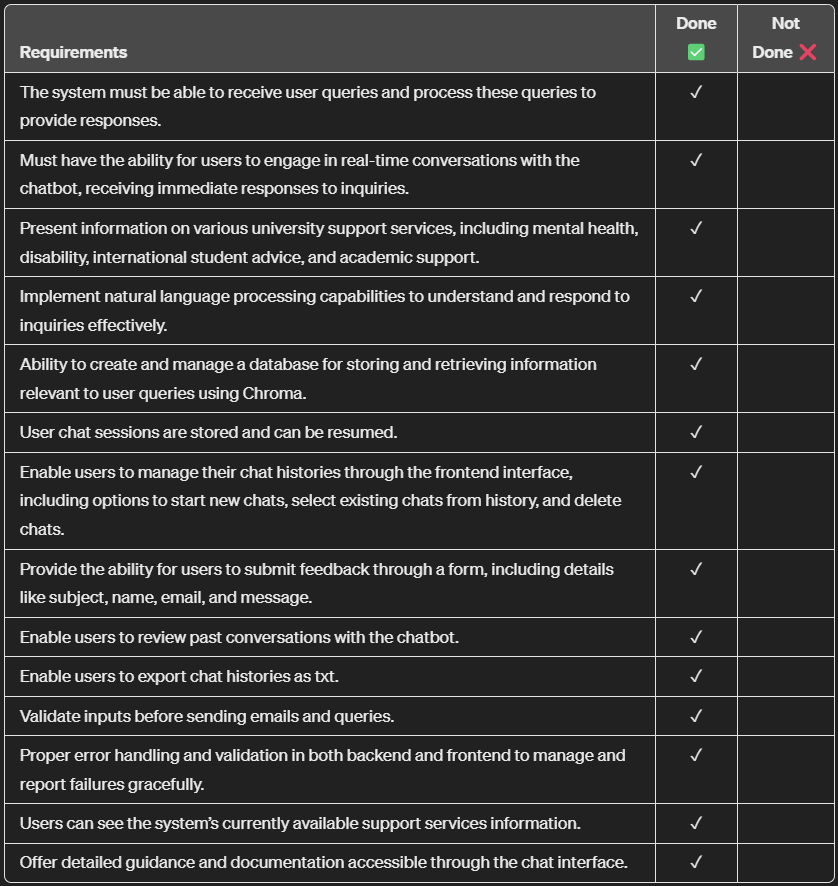
\includegraphics{images/musthave.png}
  \end{adjustbox}
  \caption{Must Have Requirements Validation.}
\end{figure}


\section*{Requirements Validation - Should Have}

\begin{figure}[h!]
  \centering
  \begin{adjustbox}{center,max height=0.53\textheight, max width=\linewidth}
    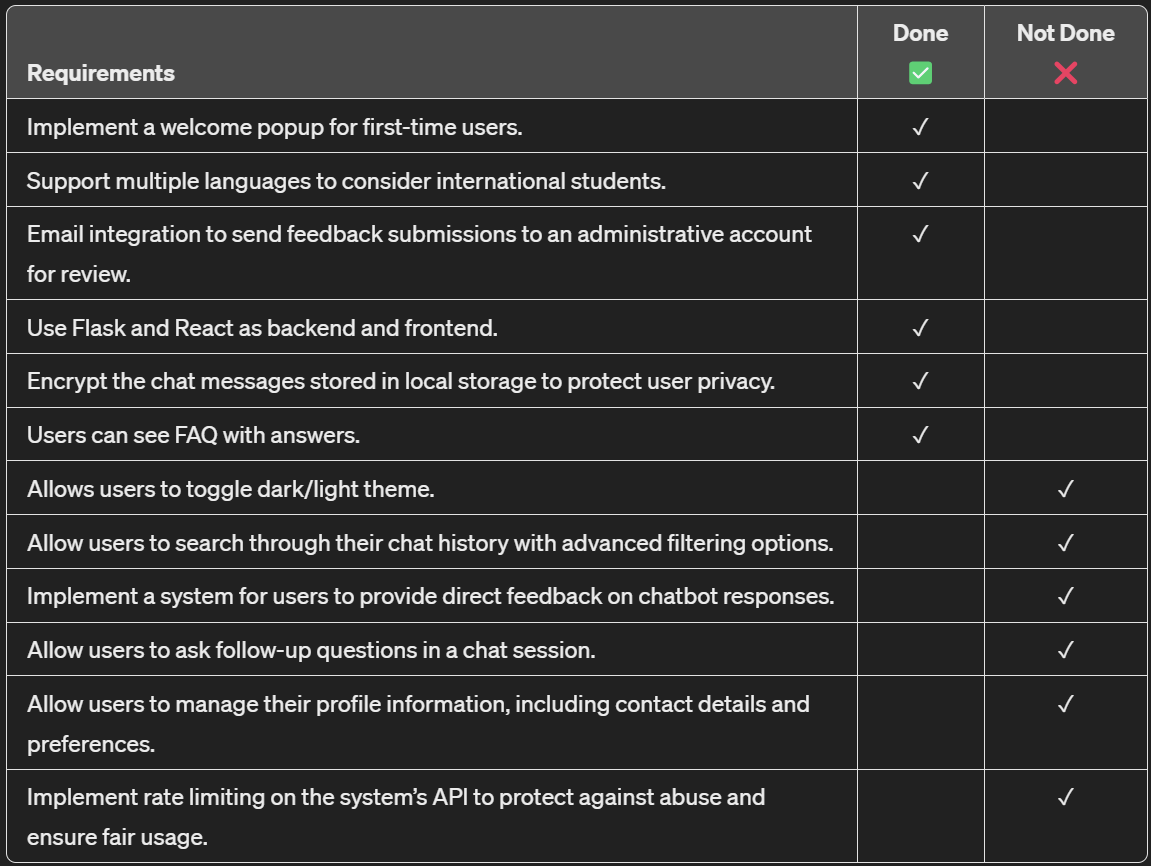
\includegraphics{images/shouldhave.png}
  \end{adjustbox}
  \caption{Should Have Requirements Validation.}
\end{figure}


\chapter{Evaluation Survey}
\label{Evaluation Survey}


\begin{figure}[h!]
  \centering
  \begin{adjustbox}{center,max height=0.77\textheight, max width=\linewidth}
    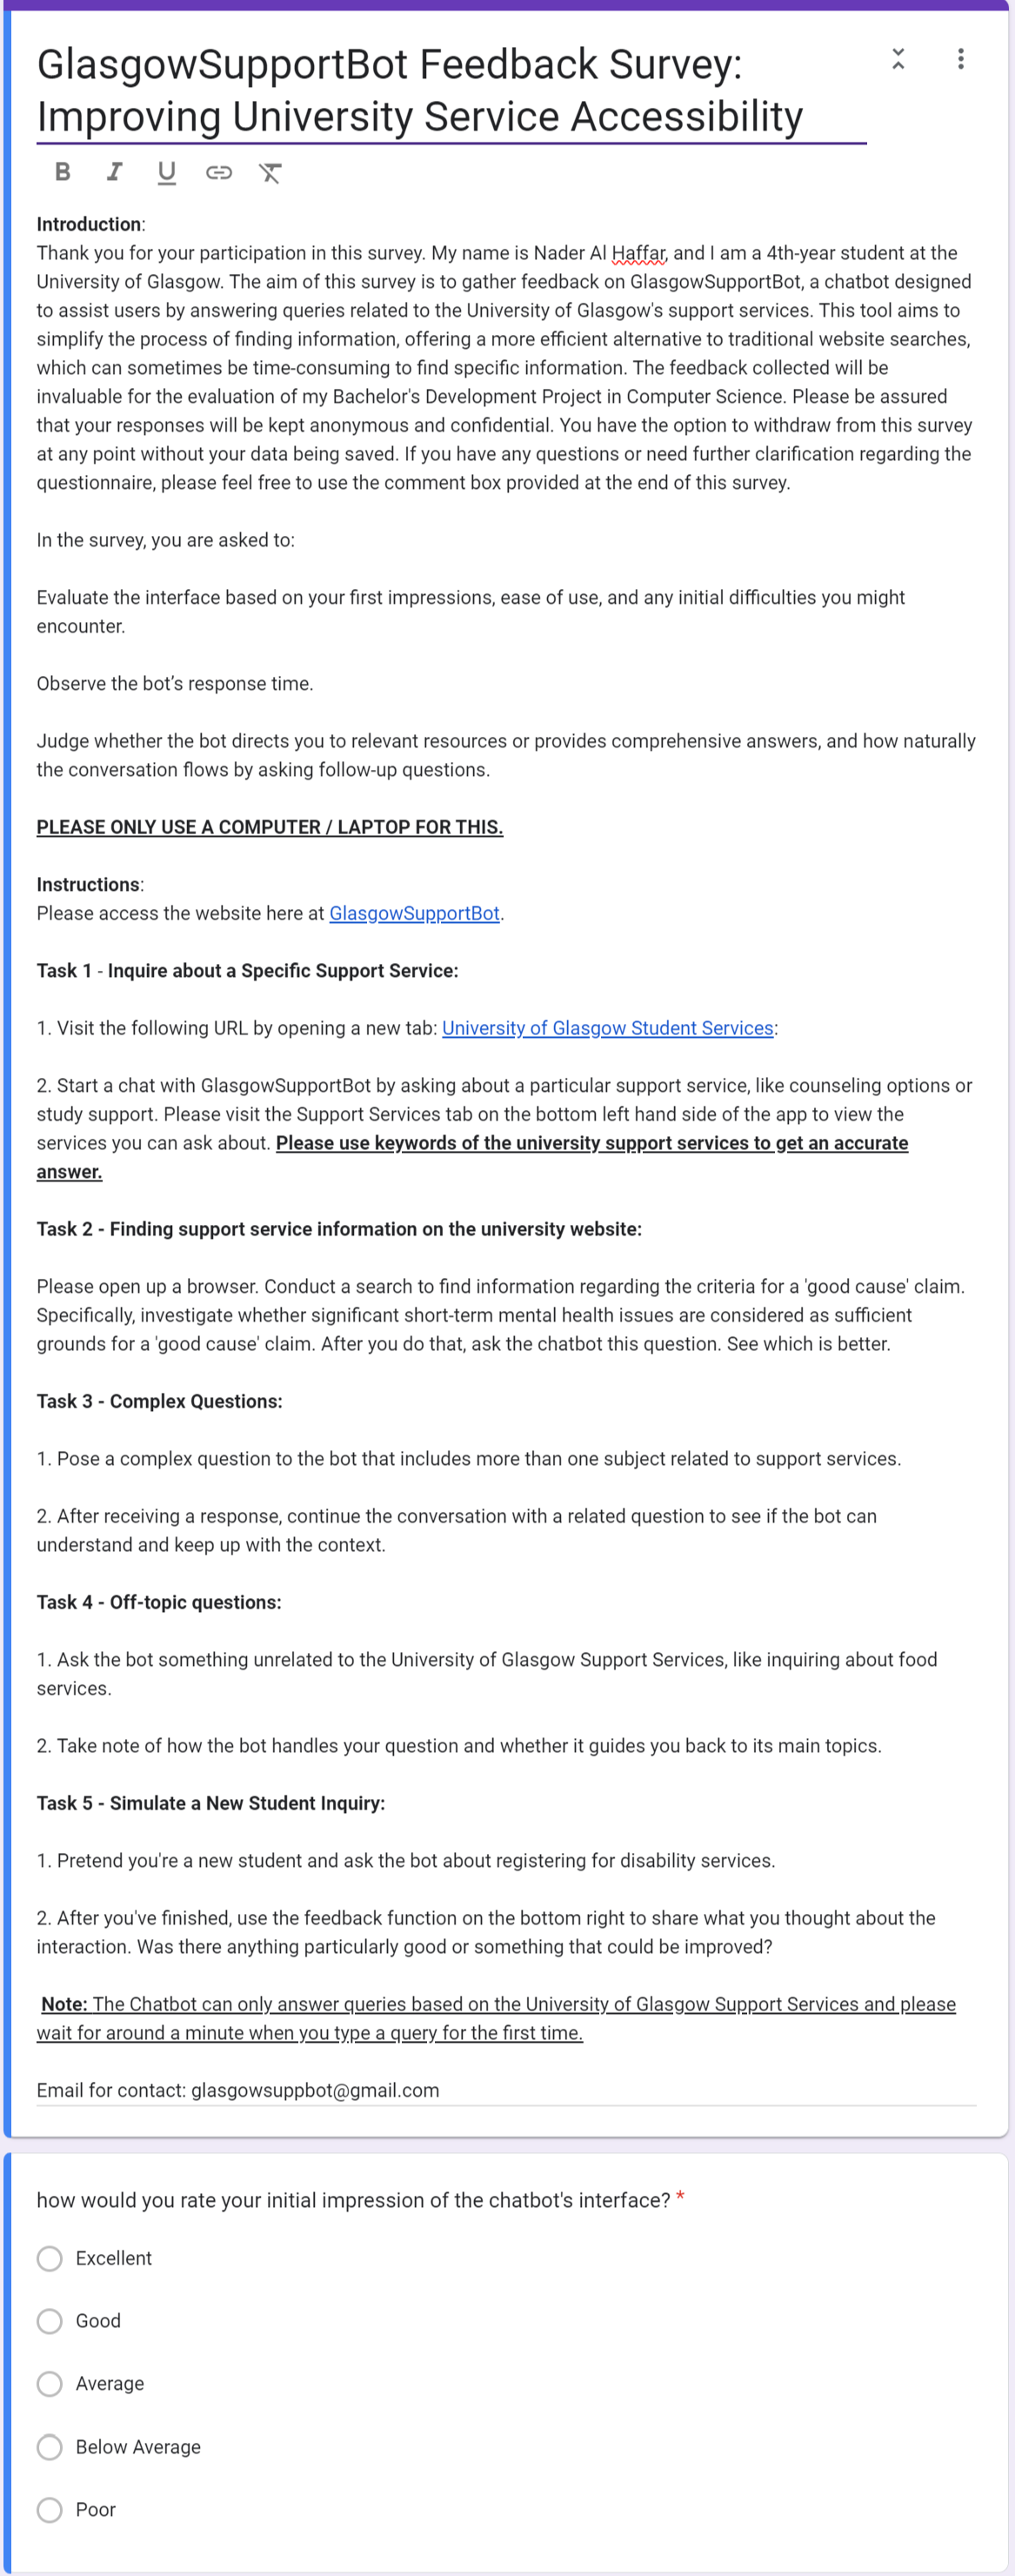
\includegraphics{images/survey1.png}
  \end{adjustbox}
  \caption{Survey Page 1.}
  \label{fig: Survey Page 1}
\end{figure}

\clearpage % Ensures the next image is on a new page

\begin{figure}[h!]
  \centering
  \begin{adjustbox}{center,max height=0.77\textheight, max width=\linewidth}
    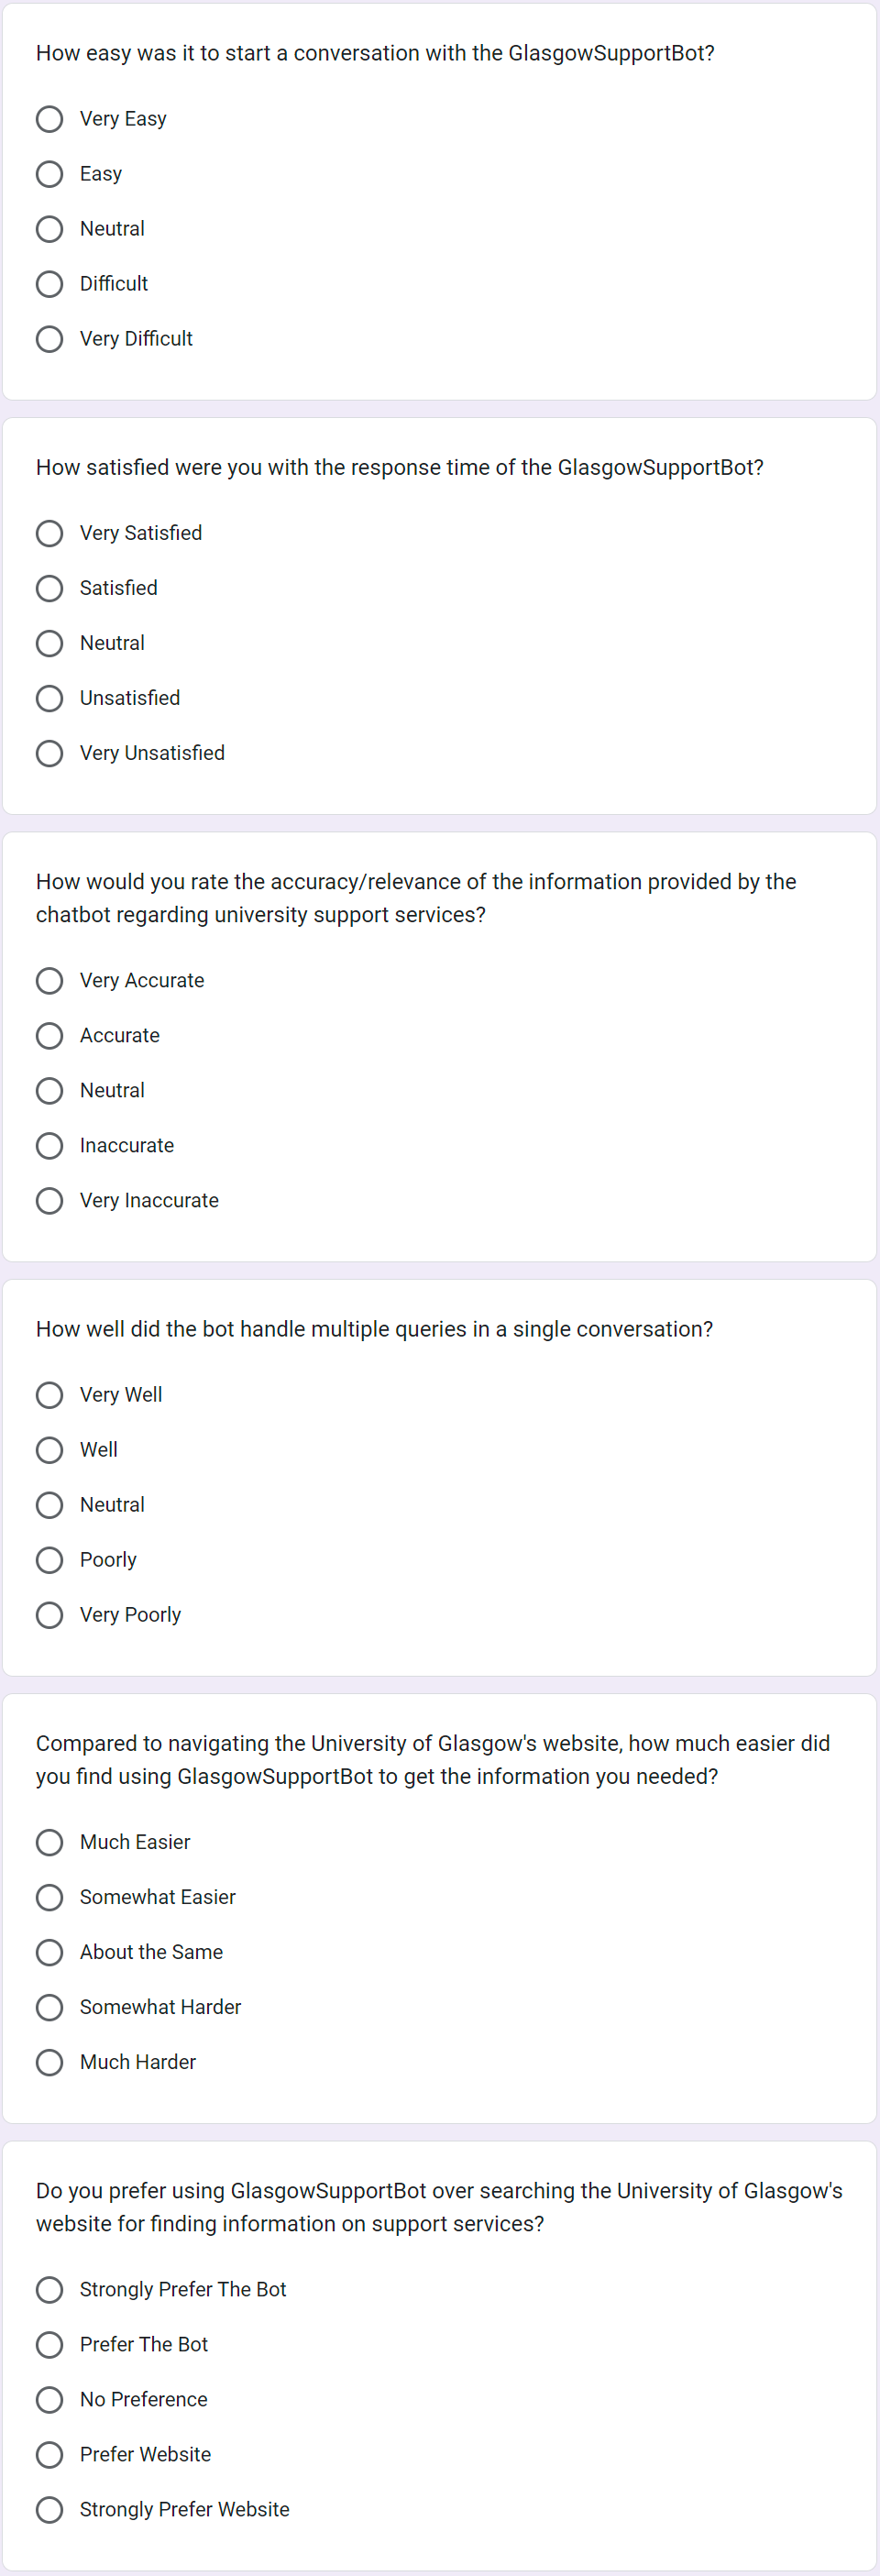
\includegraphics{images/survey2.png}
  \end{adjustbox}
  \caption{Survey Page 2.}
  \label{fig: Survey Page 2}
\end{figure}
\clearpage % Ensures the next image is on a new page

\begin{figure}[h!]
  \centering
  \begin{adjustbox}{center,max height=0.77\textheight, max width=\linewidth}
    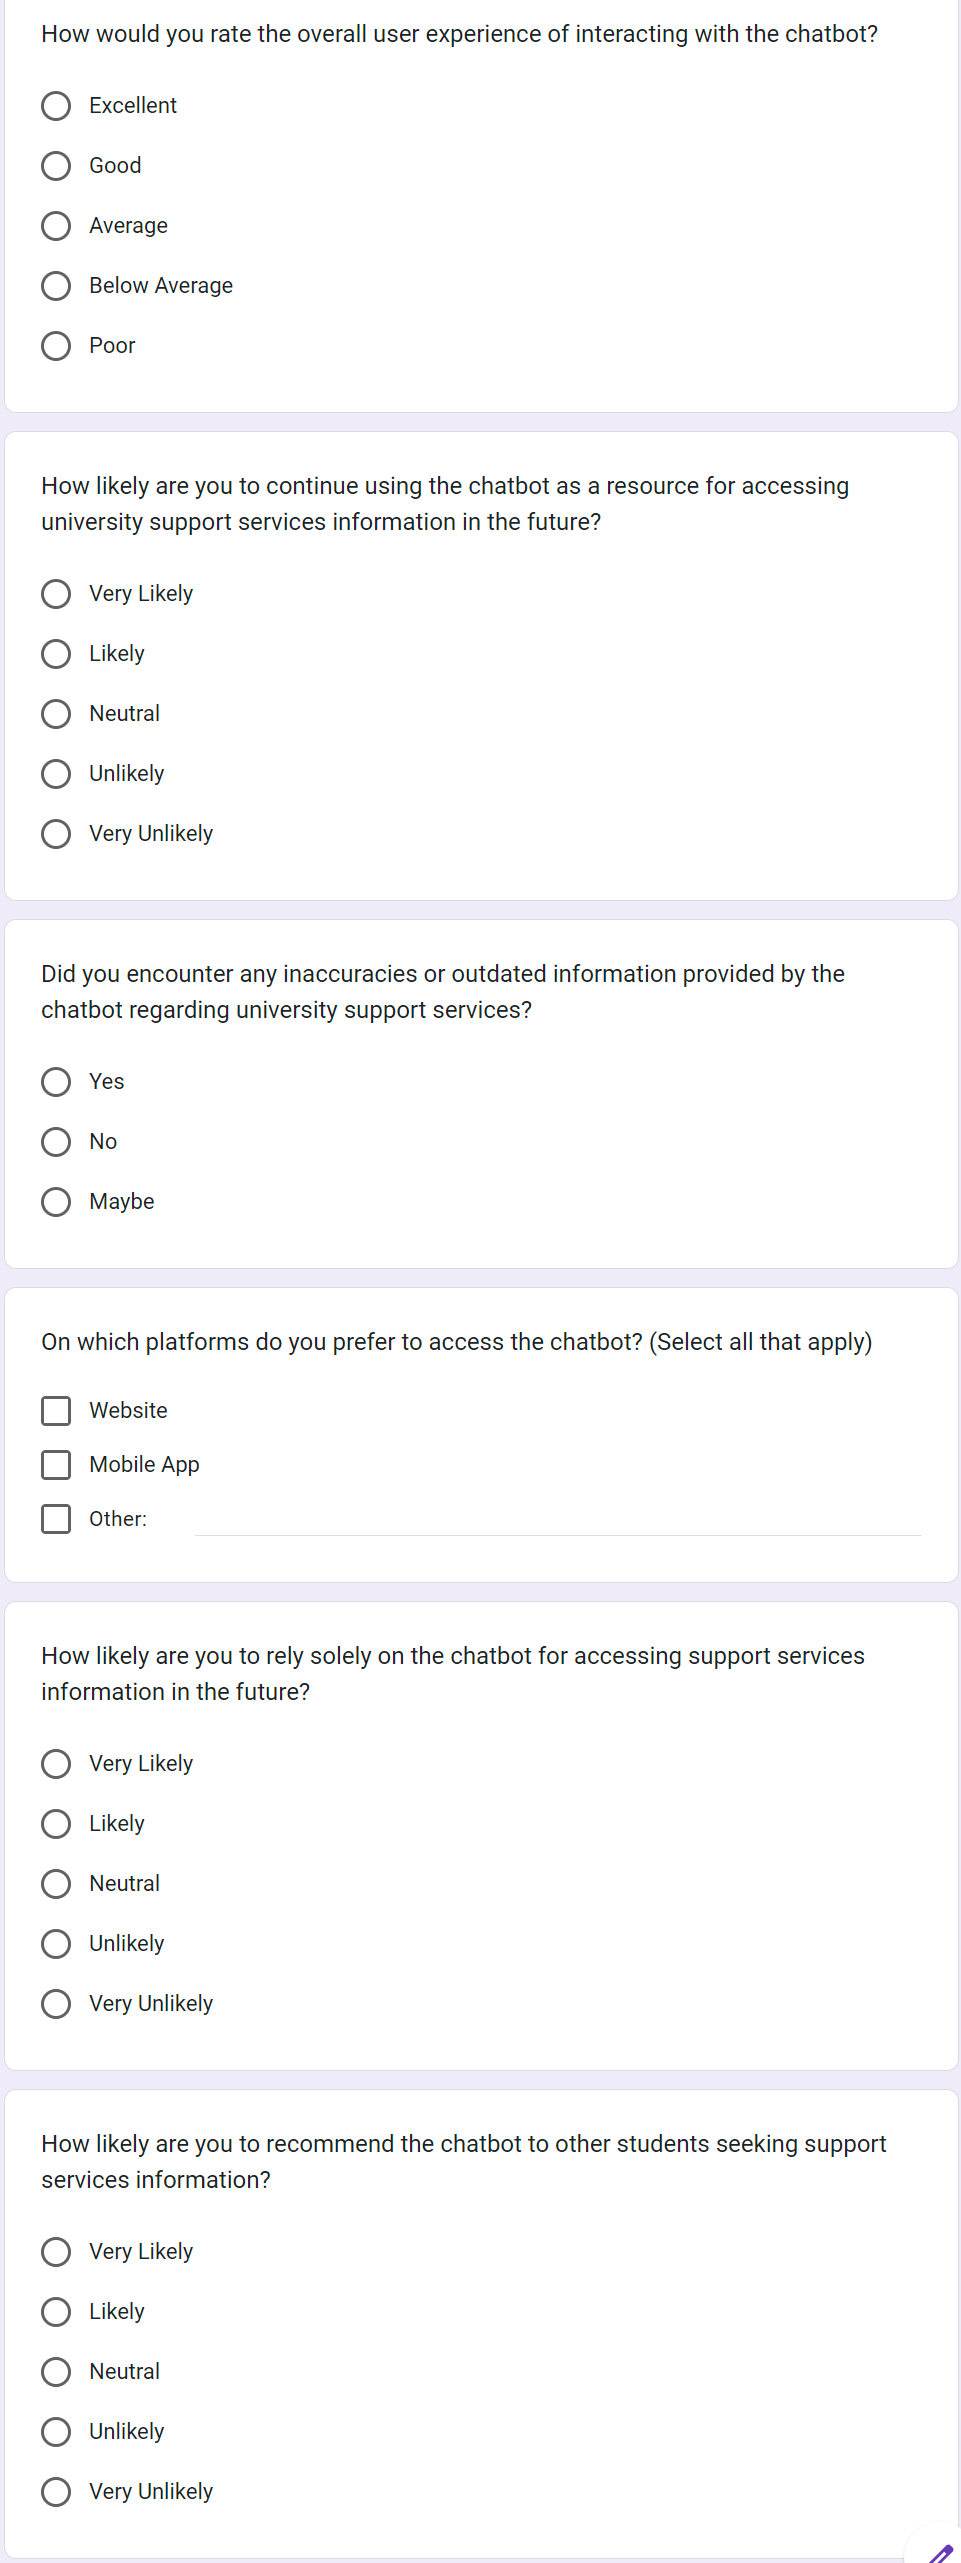
\includegraphics{images/survey3.png}
  \end{adjustbox}
  \caption{Survey Page 3.}
  \label{fig: Survey Page 1}
\end{figure}
\clearpage % Ensures the next image is on a new page

\begin{figure}[h!]
  \centering
  \begin{adjustbox}{center,max height=0.77\textheight, max width=\linewidth}
    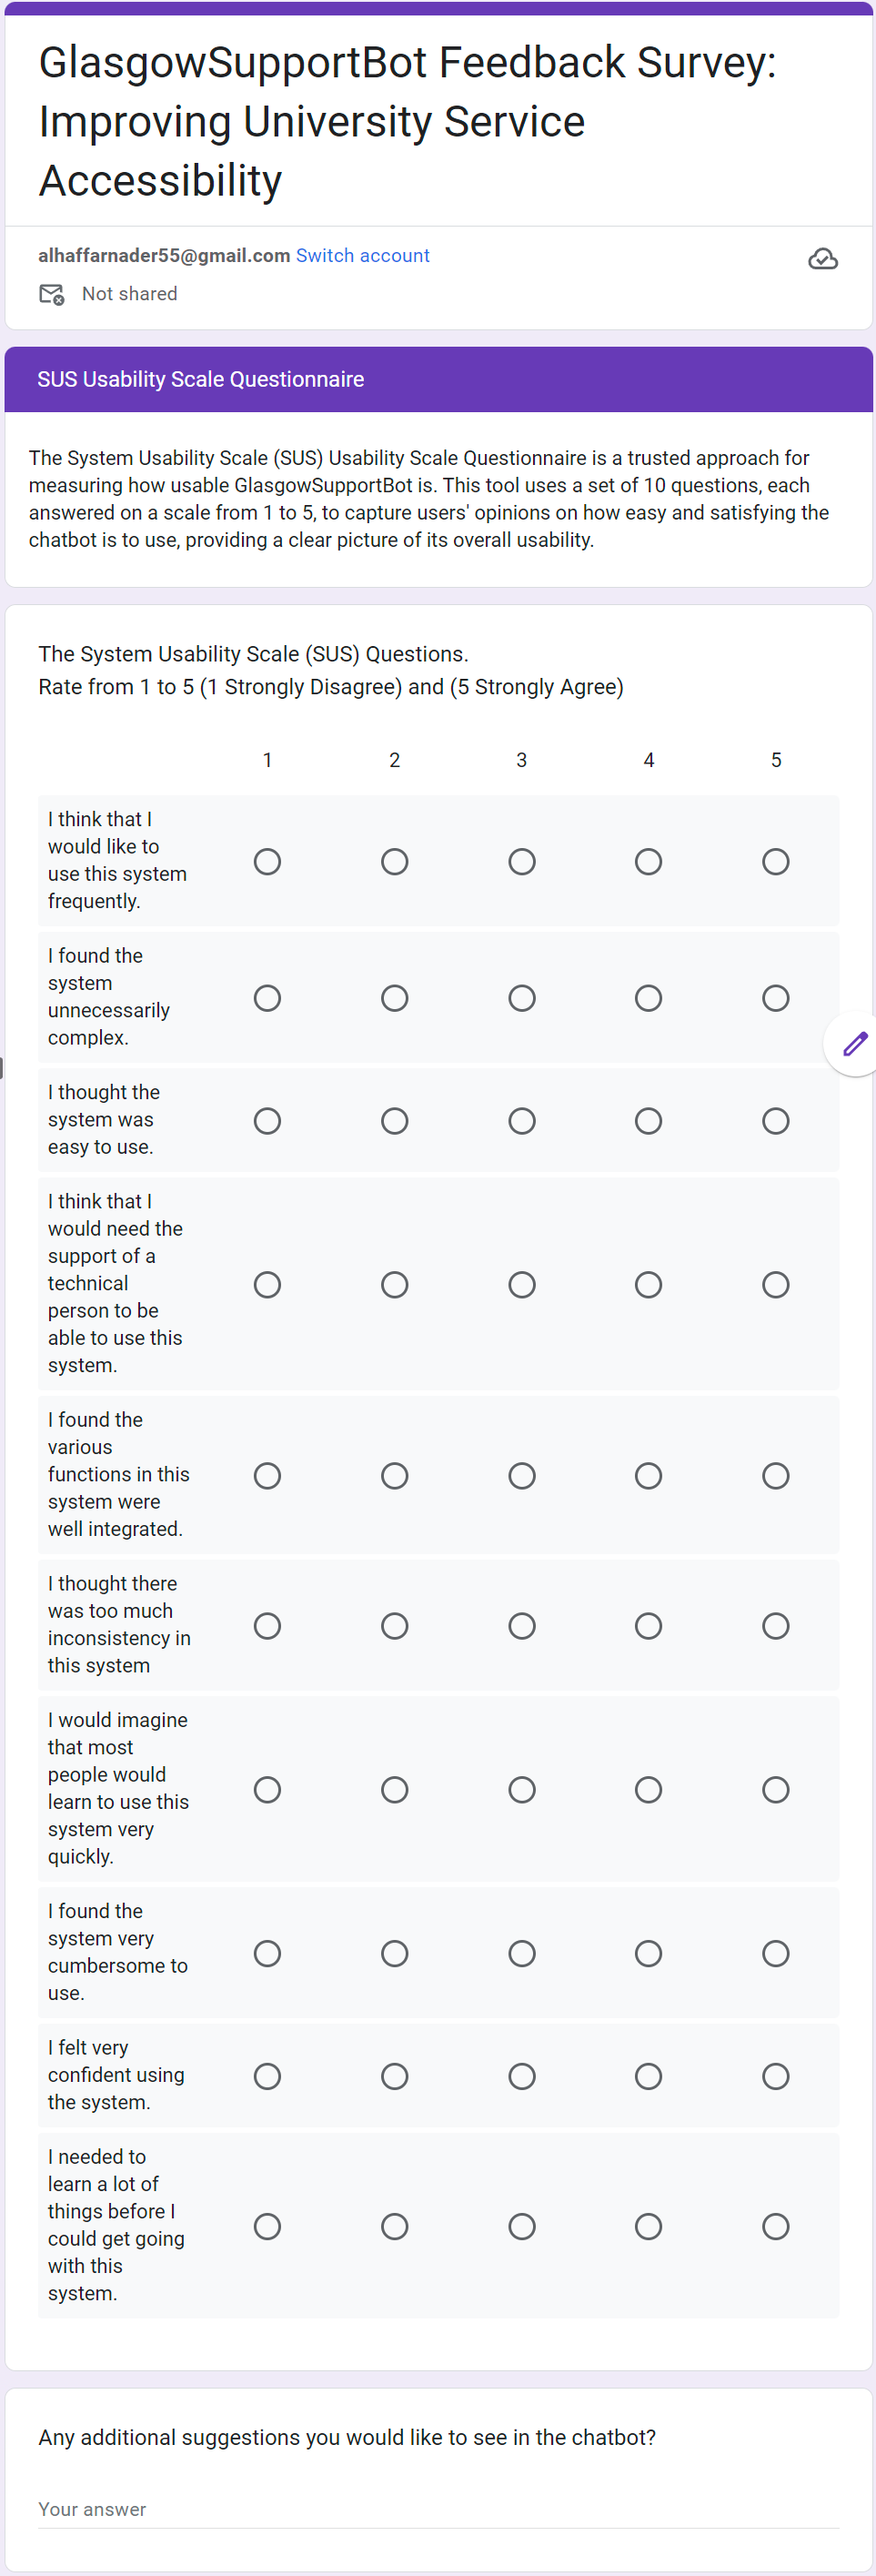
\includegraphics{images/survey4.png}
  \end{adjustbox}
  \caption{SUS Survey Page 4.}
  \label{fig: Survey Page 4}
\end{figure}

\section*{\textbf{Survey Google Forms Link}}
Please access the survey using the following link: \href{https://docs.google.com/forms/d/e/1FAIpQLSdlZLvJn7b81gKnwkcBIw-7jVdgHIu1LeQ7mDHLe96U08lMFQ/viewform?usp=sf_link}{\textbf{Survey Link}}.

\chapter{Initial Prototypes}
\label{Initial Prototypes}

In this section, the initial prototypes created at the beginning of  GlasgowSupportBot's development are displayed. From these prototypes, I have gained insights that informed better design decisions for the chatbot later on.

\begin{figure}[h!]
  \centering
  \begin{adjustbox}{center,max height=0.5\textheight, max width=\linewidth}
    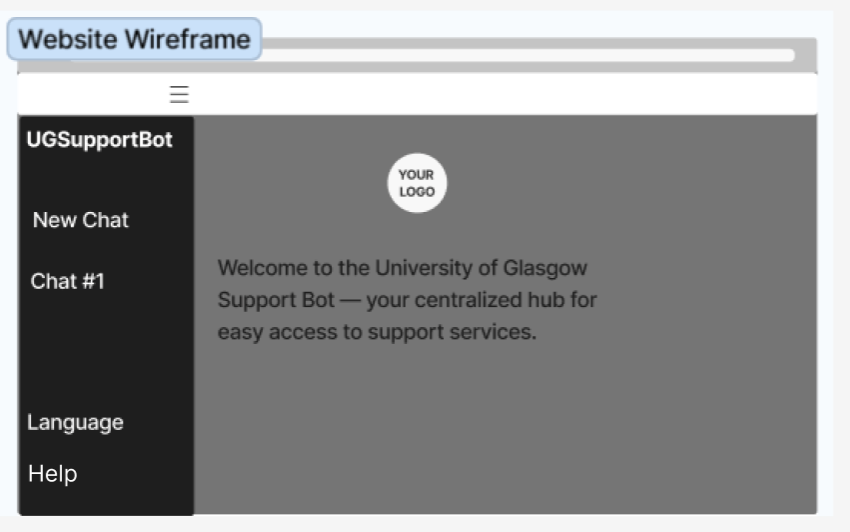
\includegraphics{images/initial1.png}
  \end{adjustbox}
  \caption{Initial prototype.}
\end{figure}

\begin{figure}[h!]
  \centering
  \begin{adjustbox}{center,max height=0.5\textheight, max width=\linewidth}
    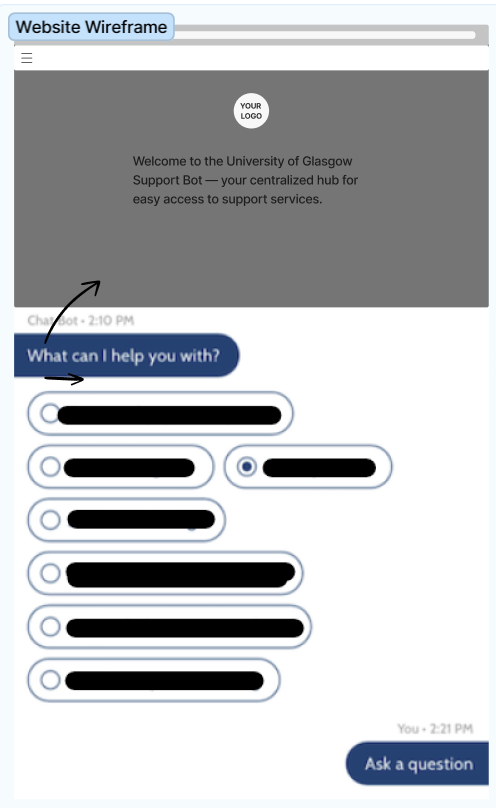
\includegraphics{images/initial2.png}
  \end{adjustbox}
  \caption{Second prototype.}
\end{figure}

\begin{figure}[h!]
  \centering
  \begin{adjustbox}{center,max height=0.35\textheight, max width=\linewidth}
    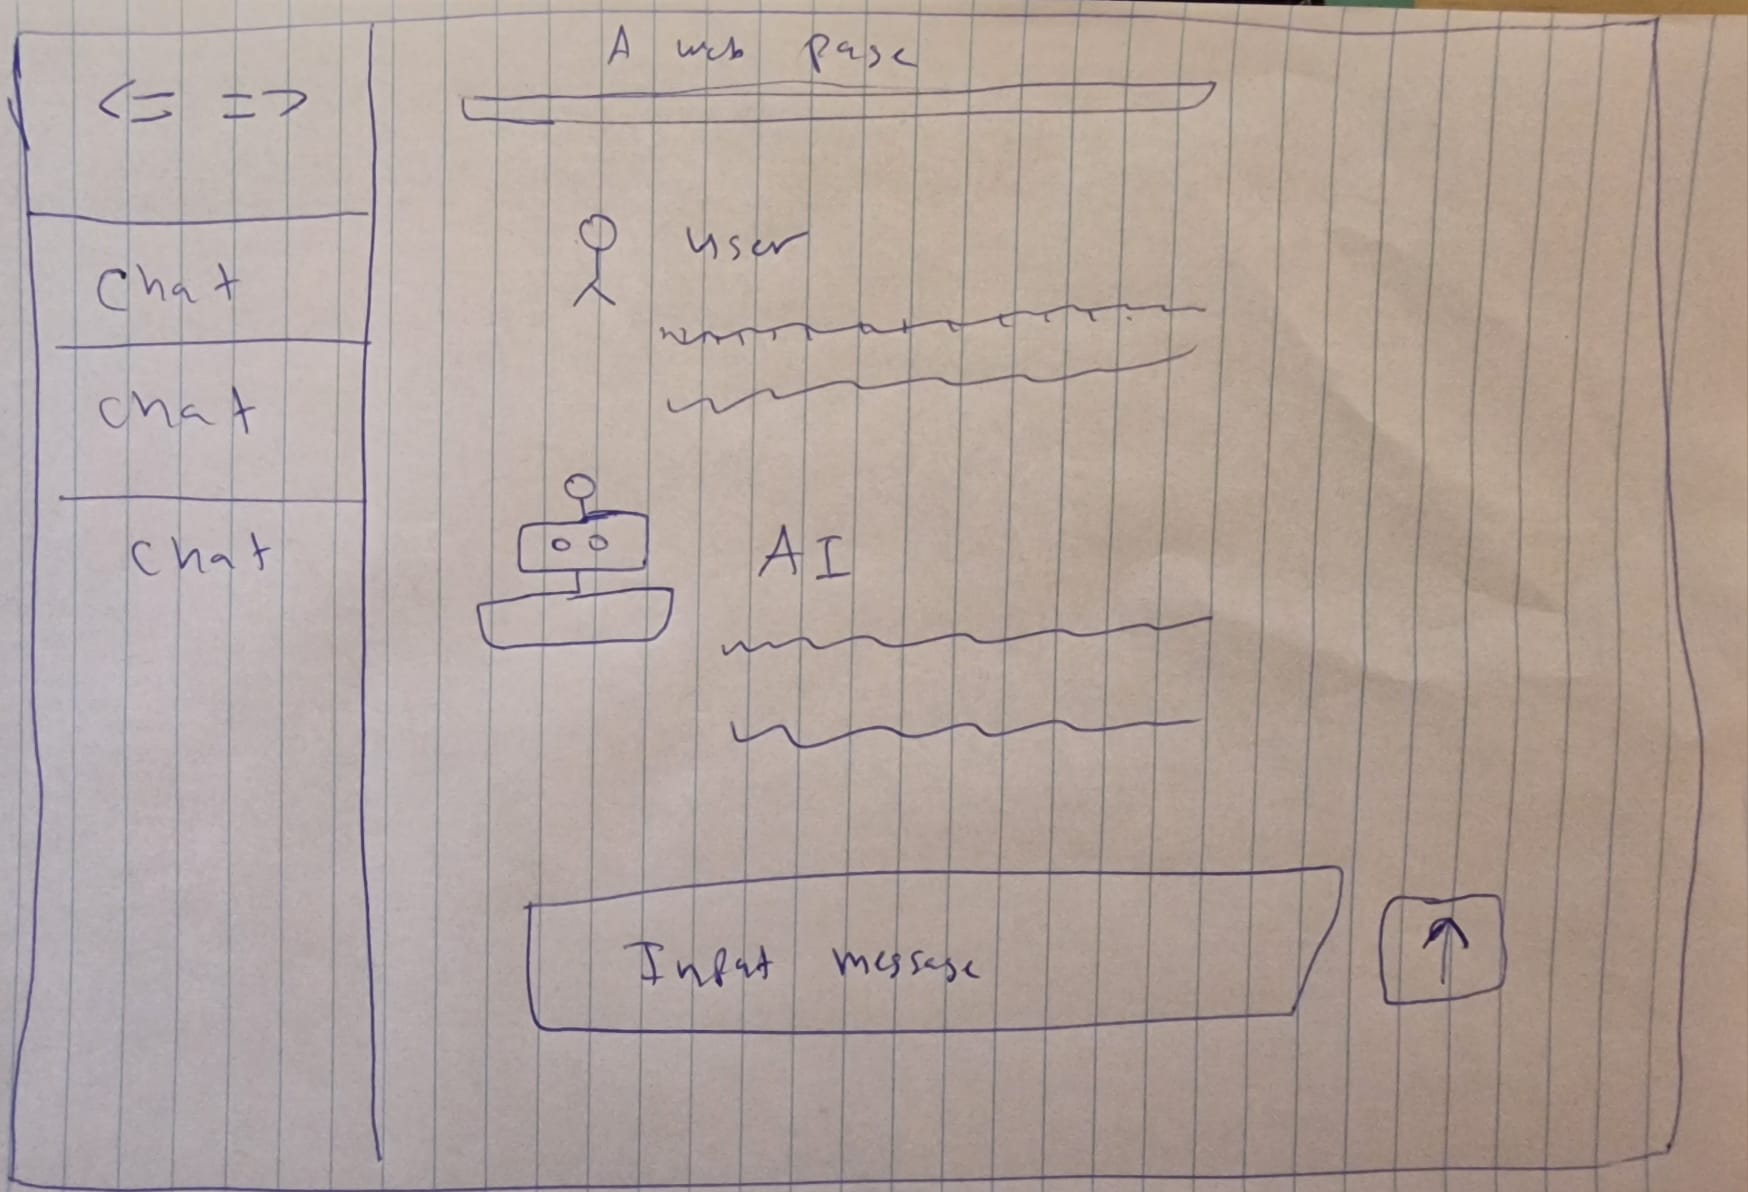
\includegraphics{images/initial3.jpeg}
  \end{adjustbox}
  \caption{Third prototype.}
\end{figure}

\chapter{Wireframe Software}
\label{Wireframe Software}

Here, we have created wireframes that consist of multiple pages, allowing for navigation through button presses. Note: Navigation to the main page can be achieved by clicking on either the chat history panel or the panel containing elements for support services, documentation, and frequently asked questions. The software used to create the wireframes is Justinmind. It is very similar to Figma.

From the top right corner, you can select and view the different wireframes as shown in picture below:
\begin{figure}[h!]
  \centering
  \begin{adjustbox}{center,max height=0.4\textheight, max width=\linewidth}
    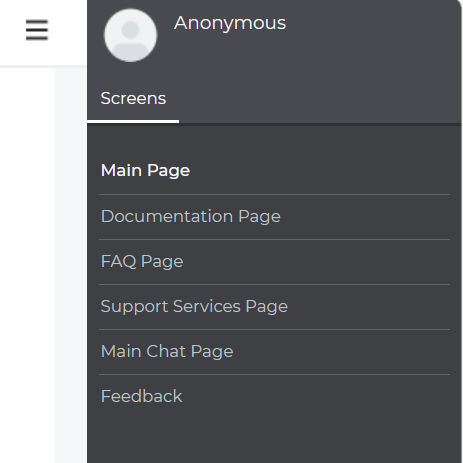
\includegraphics{images/instructionjustinmind.png}
  \end{adjustbox}
  \caption{Instruction to access the Wireframes.}
\end{figure}

Please access the wireframes using the following link: 
\href{https://cloud.justinmind.com/usernote/prototype/32f43d89128931ea5ef39043b4898b3d943f1a4d570f702c6785805d01214a34}{\textbf{Wireframes Link}}.

\chapter{Wireframes}
\label{Wireframes}

\begin{figure}[h!]
  \centering
  \begin{adjustbox}{center,max height=0.4\textheight, max width=\linewidth}
    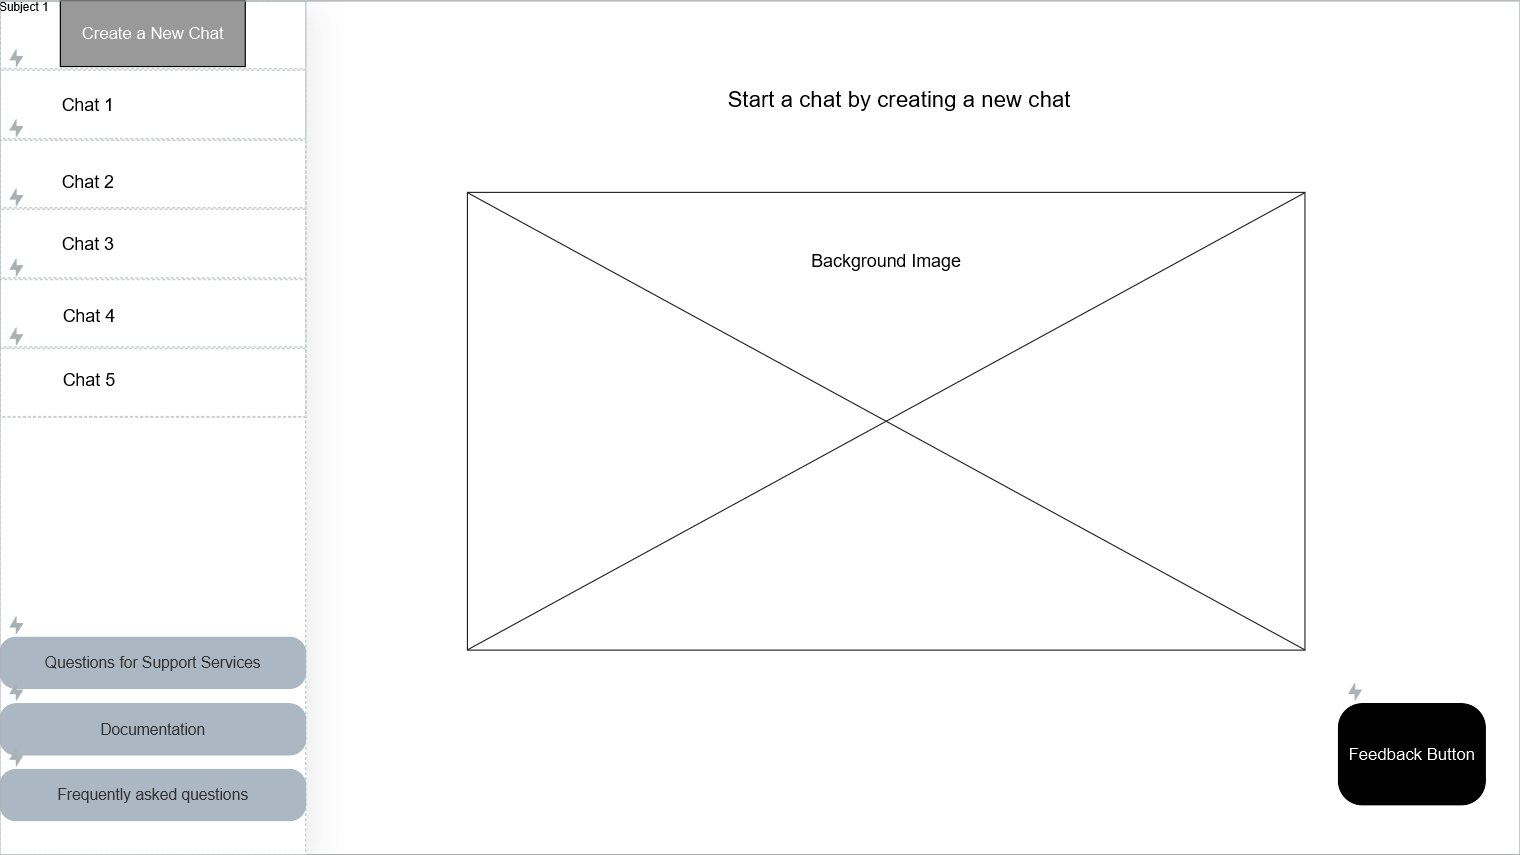
\includegraphics{images/wireframebackgroundpage.png}
  \end{adjustbox}
  \caption{Default Page.}
\end{figure}

\begin{figure}[h!]
  \centering
  \begin{adjustbox}{center,max height=0.4\textheight, max width=\linewidth}
    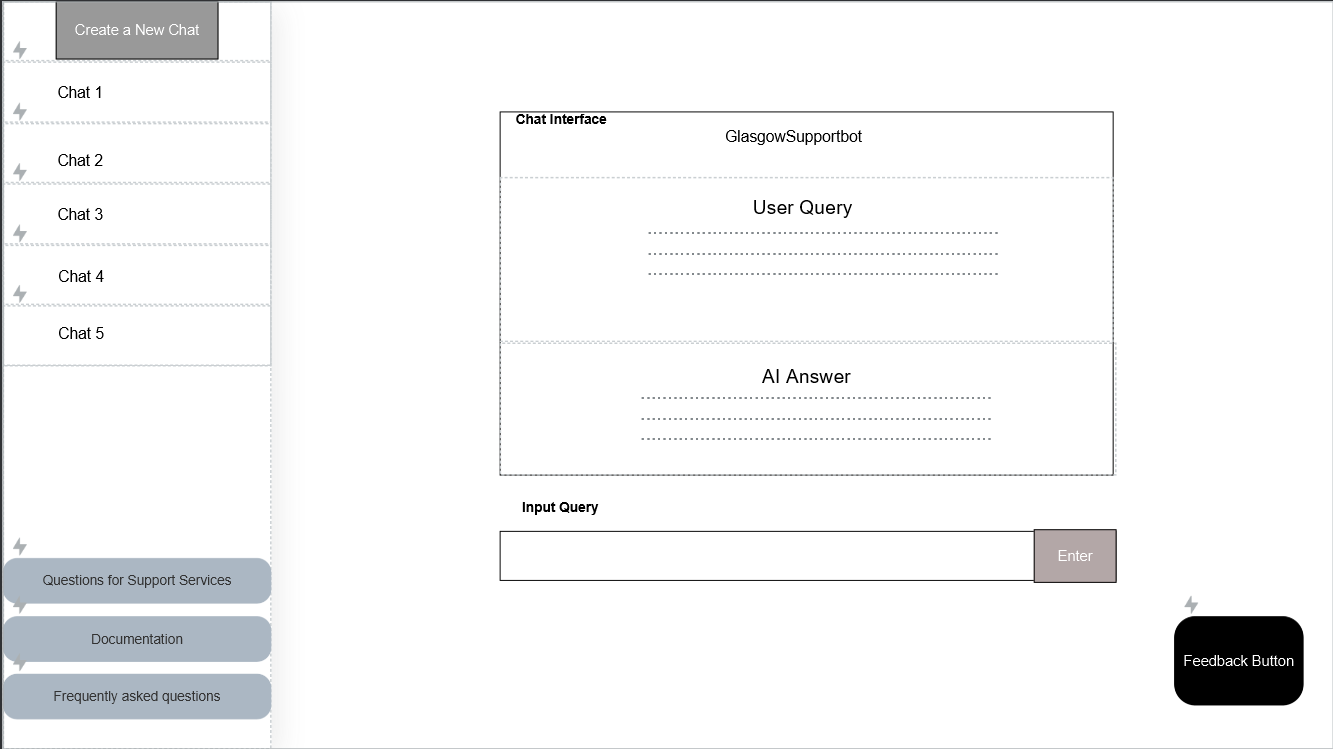
\includegraphics{images/wireframechatpage.png}
  \end{adjustbox}
  \caption{Chat Page.}
\end{figure}

\begin{figure}[h!]
  \centering
  \begin{adjustbox}{center,max height=0.4\textheight, max width=\linewidth}
    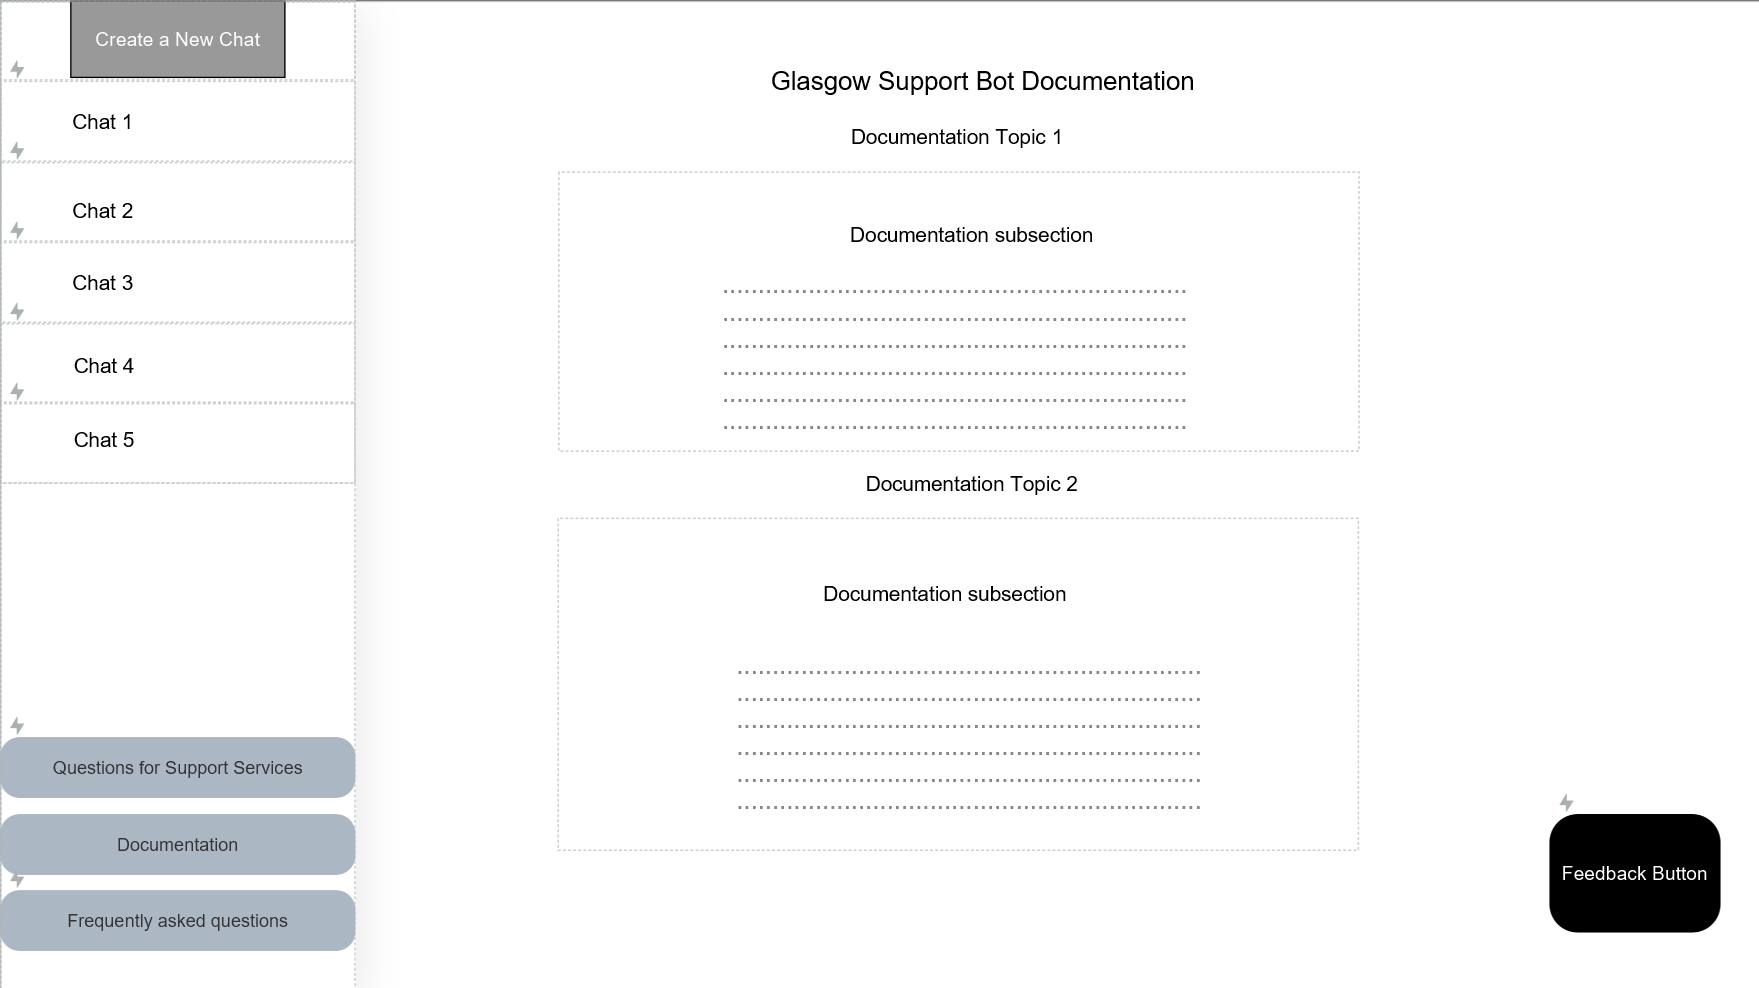
\includegraphics{images/wireframedocpage.png}
  \end{adjustbox}
  \caption{Documentation Page.}
\end{figure}

\begin{figure}[h!]
  \centering
  \begin{adjustbox}{center,max height=0.4\textheight, max width=\linewidth}
    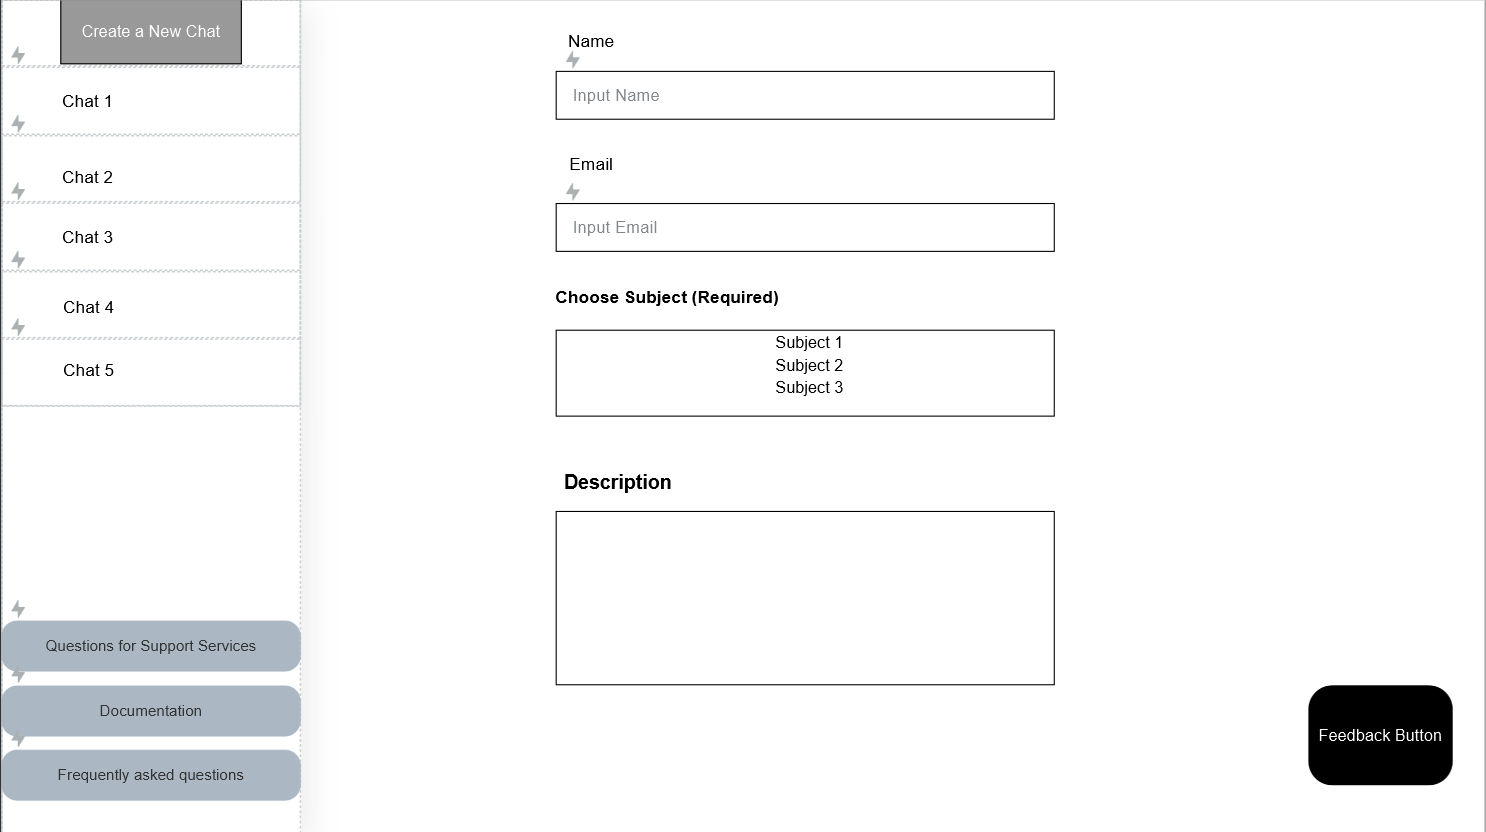
\includegraphics{images/wireframecfeedbackpage.png}
  \end{adjustbox}
  \caption{Feedback Interface.}
\end{figure}


\begin{figure}[h!]
  \centering
  \begin{adjustbox}{center,max height=0.4\textheight, max width=\linewidth}
    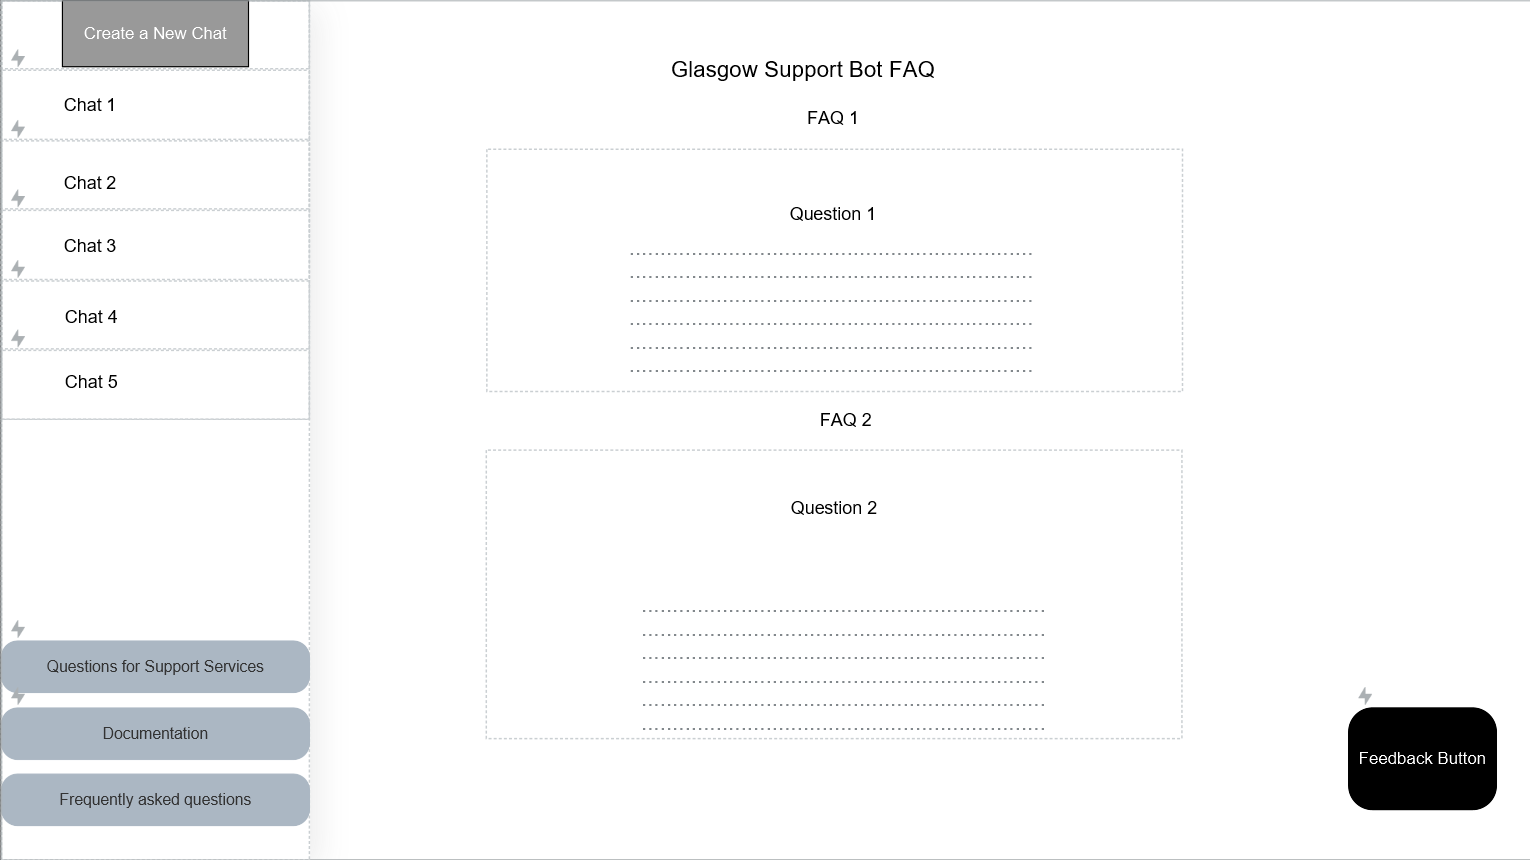
\includegraphics{images/wireframefaqpage.png}
  \end{adjustbox}
  \caption{FAQ Page.}
\end{figure}

\begin{figure}[h!]
  \centering
  \begin{adjustbox}{center,max height=0.4\textheight, max width=\linewidth}
    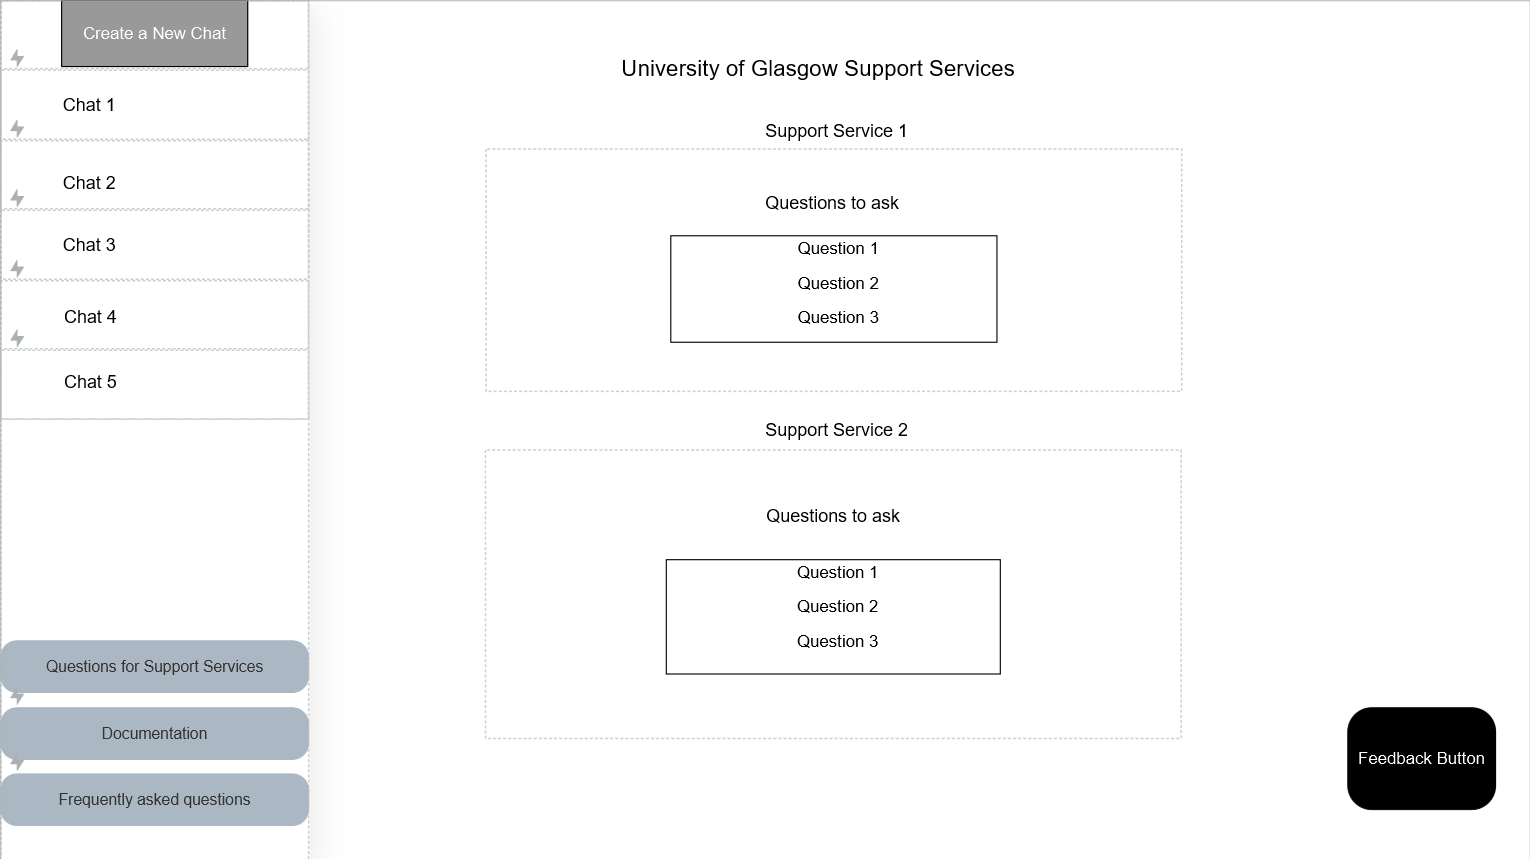
\includegraphics{images/wireframesupppage.png}
  \end{adjustbox}
  \caption{Support Services Page.}
\end{figure}

\chapter{Activity Diagram}
\label{Activity Diagram}

\begin{figure}[h!]
  \centering
  \begin{adjustbox}{center,max height=0.60\textheight, max width=\linewidth}
    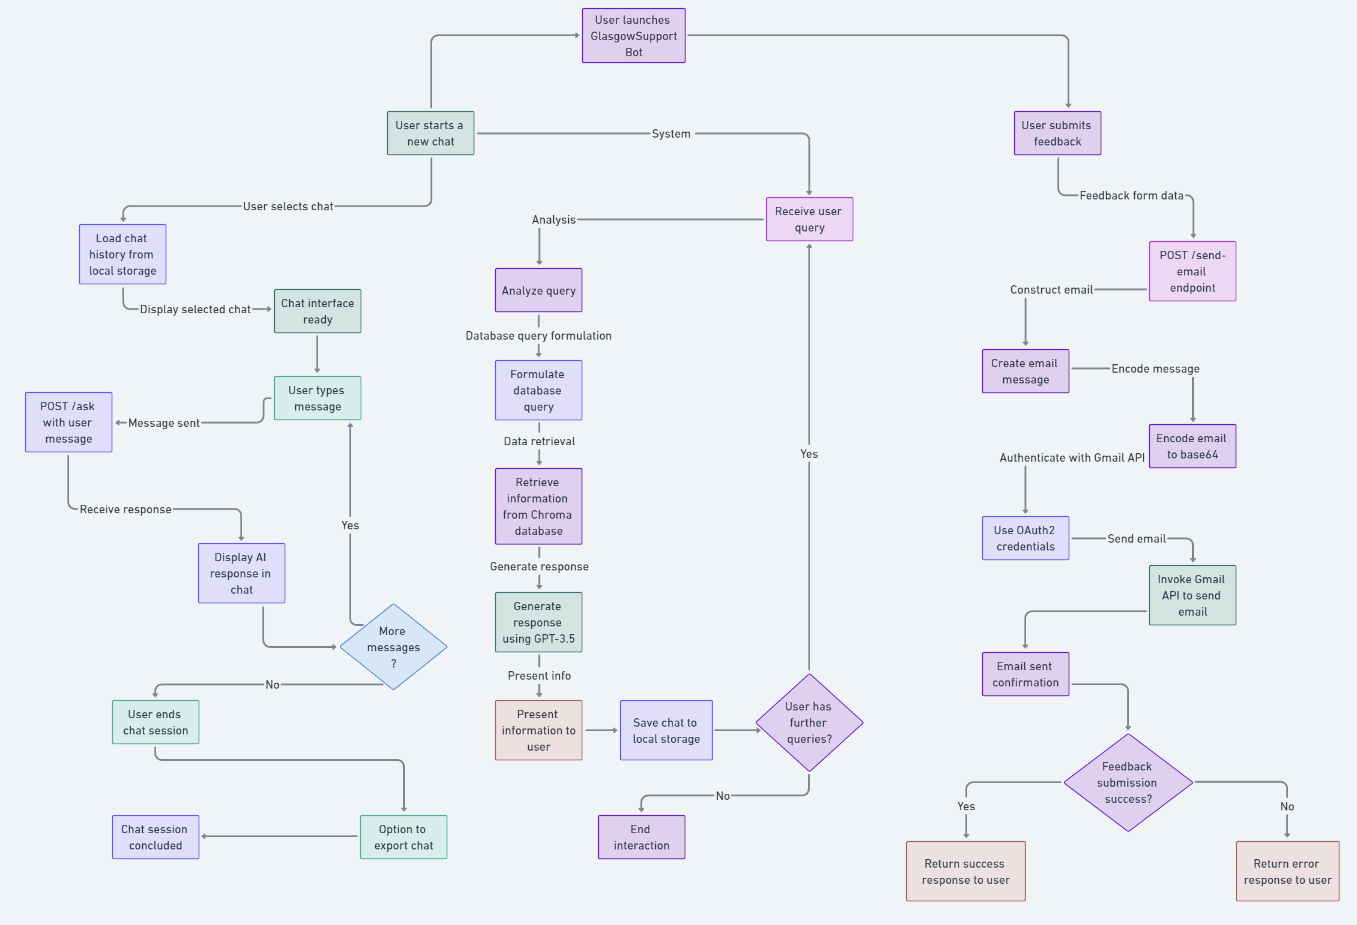
\includegraphics{images/activitydiagram.png}
  \end{adjustbox}
  \caption{Activity Diagram.}
  \label{fig:activitydiagram}
\end{figure}

\chapter{ER Diagram}
\label{ER Diagram}

\begin{figure}[h!]
  \centering
  \begin{adjustbox}{center,max height=0.4\textheight, max width=\linewidth}
    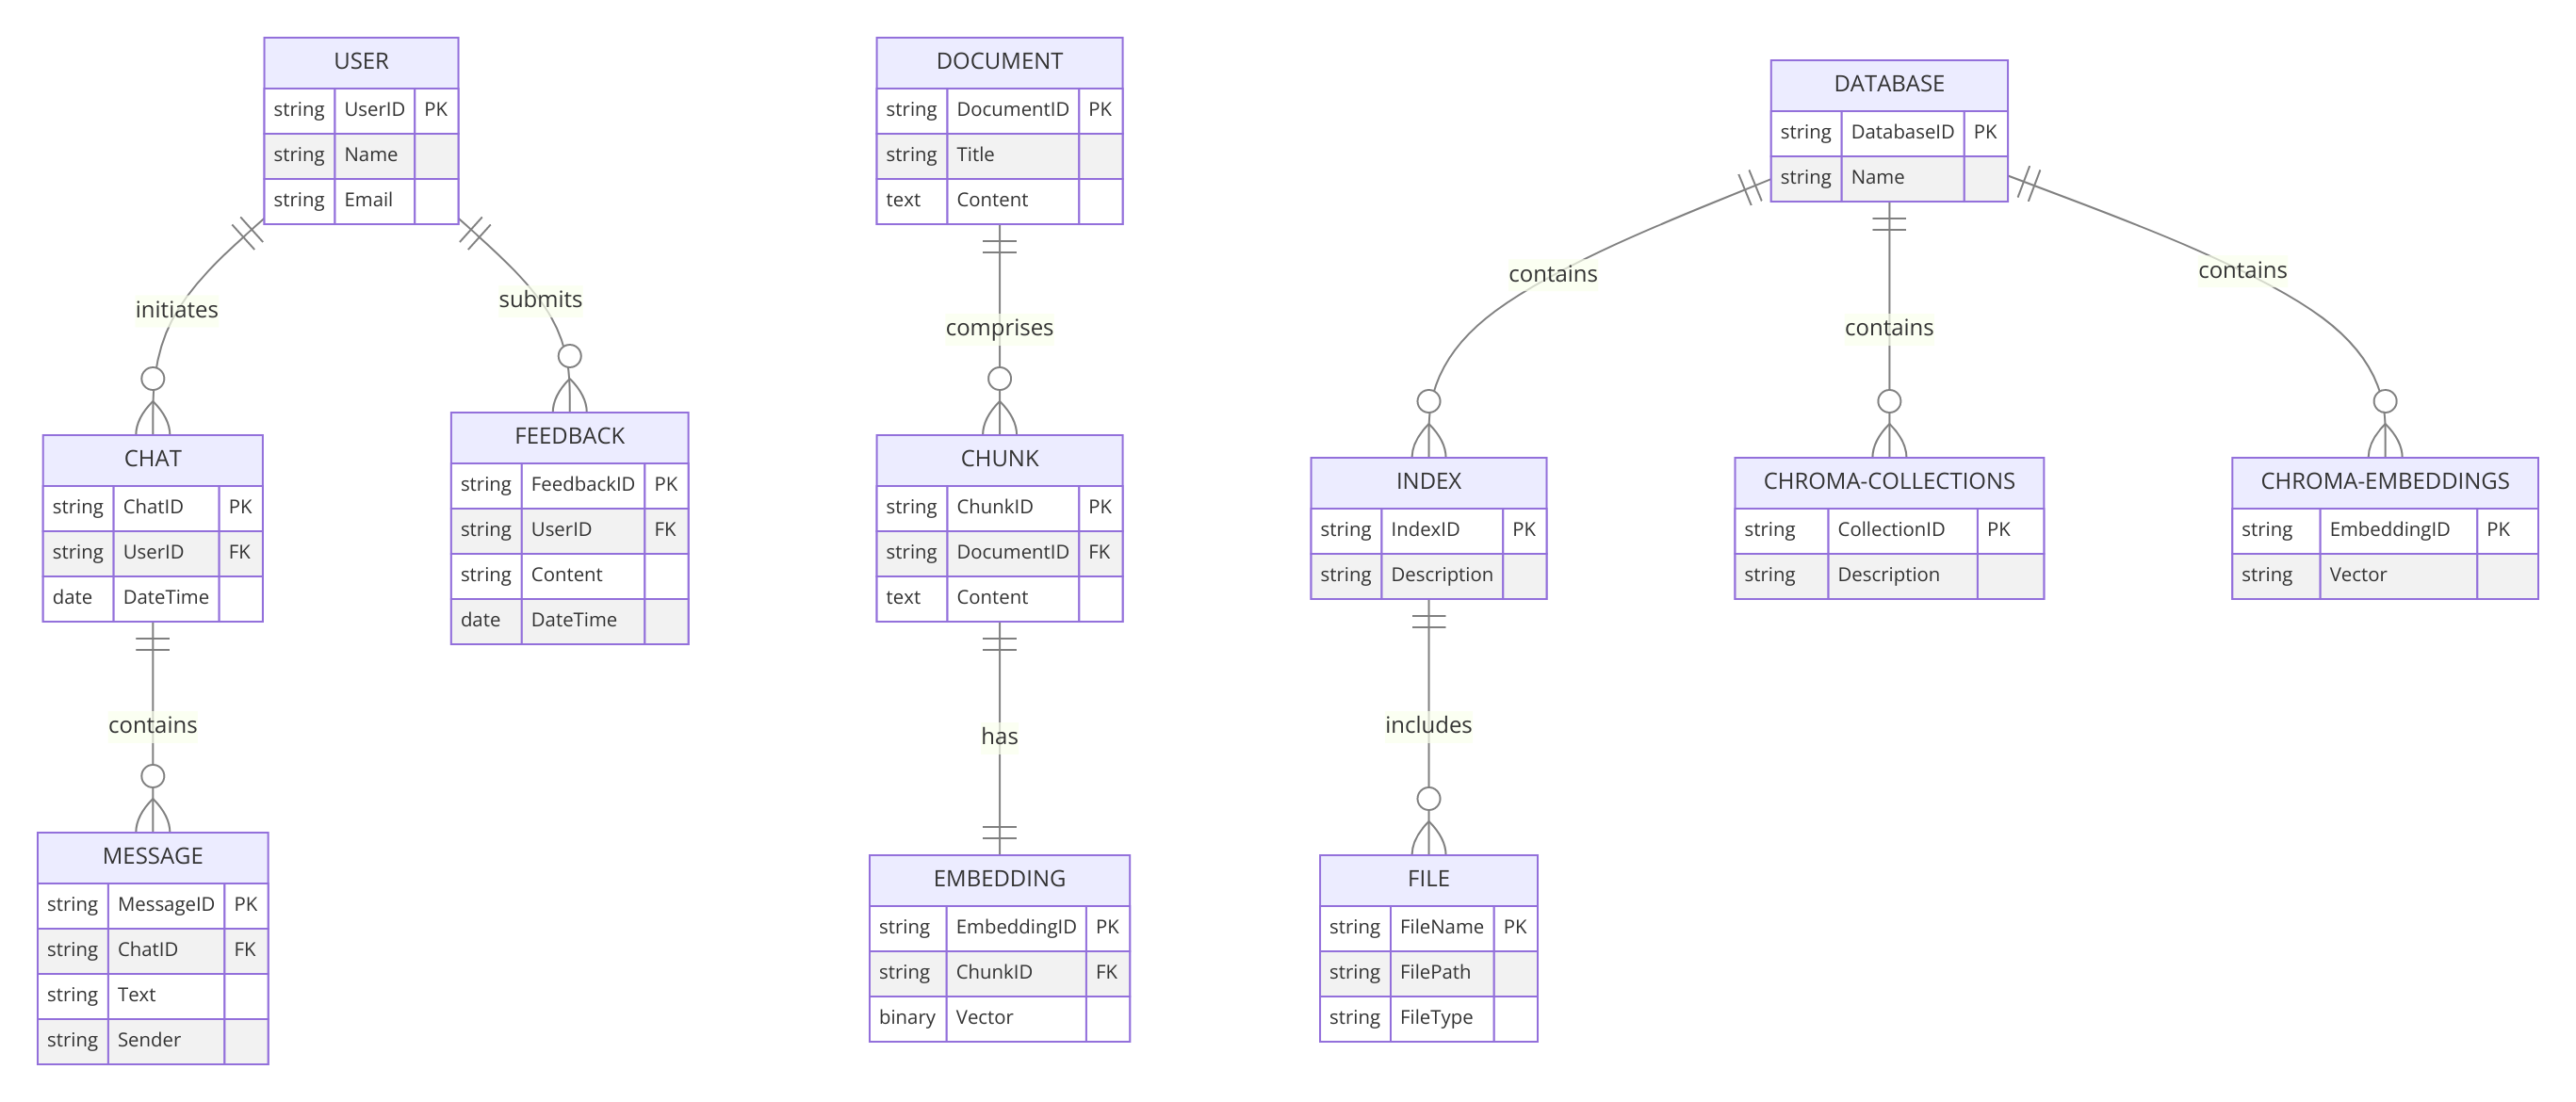
\includegraphics{images/ER Diagram.png}
  \end{adjustbox}
  \caption{ER Diagram.}
  \label{fig:ER Diagram}
\end{figure}


\chapter{Sequence Diagram}
\label{Sequence Diagram}

\begin{figure}[h!]
  \centering
  \begin{adjustbox}{center,max height=0.45\textheight, max width=\linewidth}
    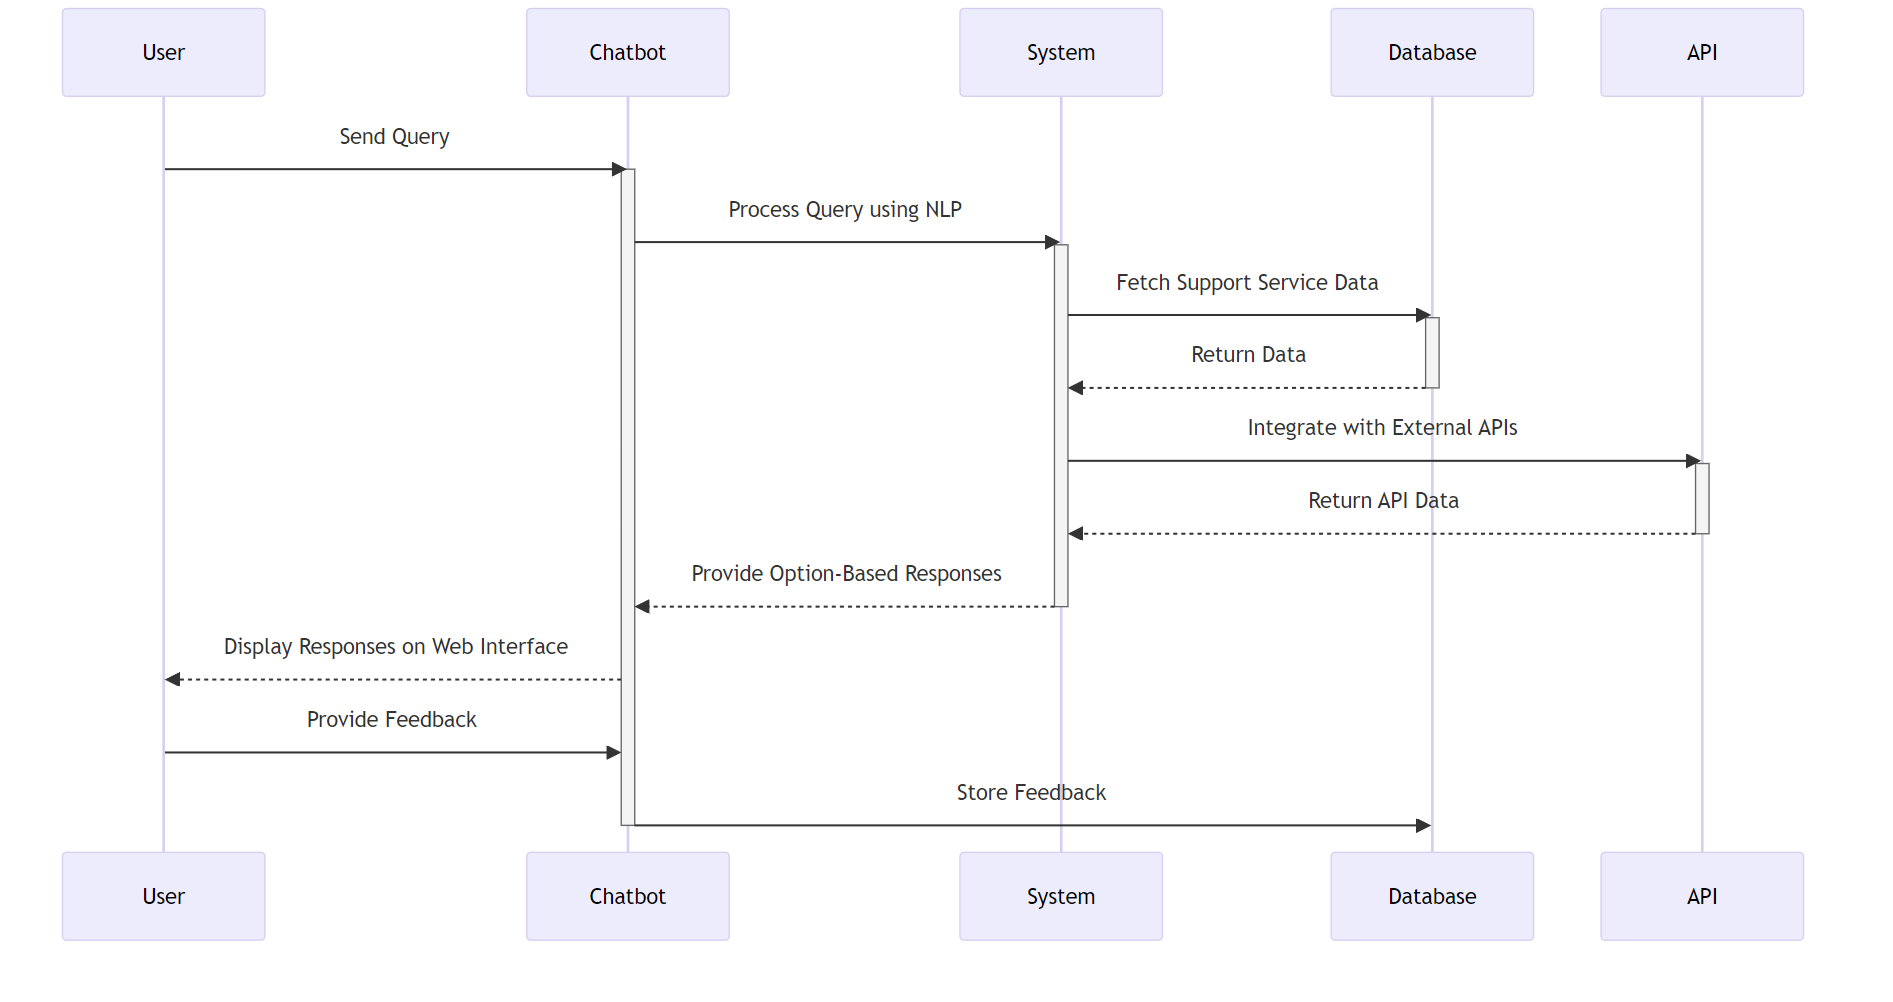
\includegraphics{images/sequencediagram.png}
  \end{adjustbox}
  \caption{Sequence Diagram.}
  \label{fig:Sequence Diagram}
\end{figure}

\chapter{Use Case Diagram}
\label{Use Case Diagram}

\begin{figure}[h!]
  \centering
  \begin{adjustbox}{center,max height=0.6\textheight, max width=\linewidth}
    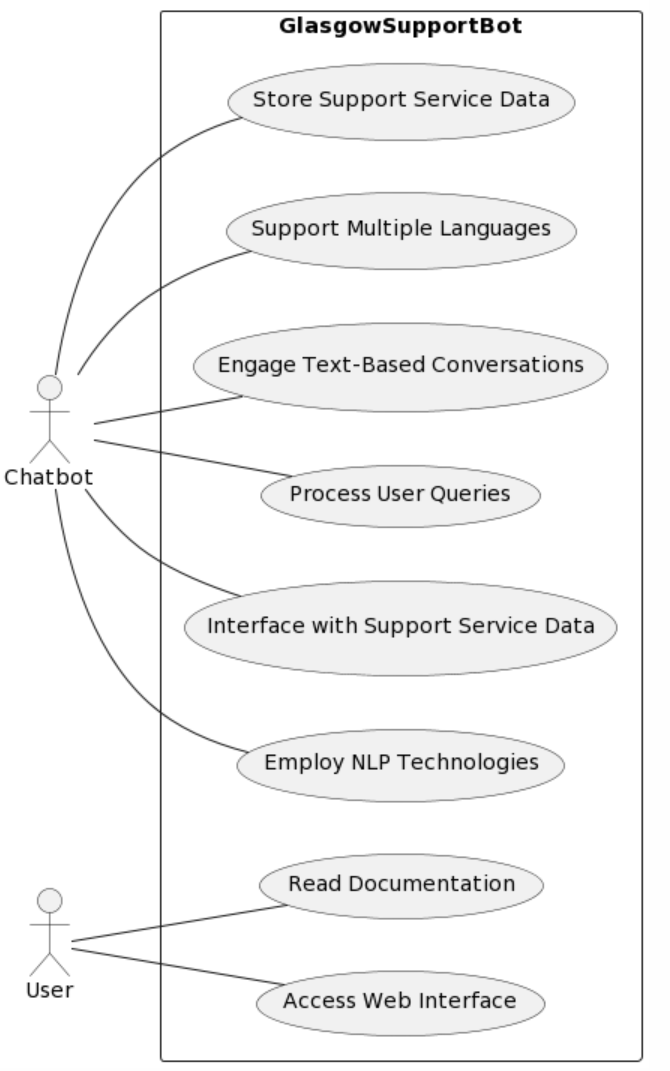
\includegraphics{images/usecase.png}
  \end{adjustbox}
  \caption{Use Case Diagram.}
  \label{fig:usecasediagram}
\end{figure}

\chapter{System Usability Student Results}
\label{System Usability Student Results}

\begin{table}[htbp]
  \centering
  \begin{tabular}{cccccccccccccc}
    \toprule
    Participant & Q1 & Q2 & Q3 & Q4 & Q5 & Q6 & Q7 & Q8 & Q9 & Q10 & Total Points & SUS Score \\
    \midrule
    Student 1 & 5 & 2 & 5 & 1 & 4 & 2 & 5 & 1 & 5 & 2 & 36 & 90.0 \\
    Student 2 & 4 & 1 & 5 & 1 & 4 & 1 & 5 & 1 & 5 & 1 & 38 & 95.0 \\
    Student 3 & 4 & 2 & 4 & 2 & 4 & 1 & 5 & 1 & 5 & 2 & 34 & 85.0 \\
    Student 4 & 3 & 1 & 5 & 1 & 4 & 2 & 5 & 1 & 5 & 2 & 35 & 87.5 \\
    Student 5 & 3 & 1 & 5 & 1 & 4 & 2 & 5 & 2 & 5 & 1 & 35 & 87.5 \\
    Student 6 & 3 & 2 & 4 & 2 & 4 & 2 & 4 & 3 & 5 & 2 & 29 & 72.5 \\
    Student 7 & 5 & 1 & 5 & 2 & 4 & 2 & 4 & 2 & 4 & 1 & 34 & 85.0 \\
    Student 8 & 4 & 2 & 5 & 1 & 5 & 1 & 5 & 2 & 4 & 1 & 36 & 90.0 \\
    Student 9 & 5 & 1 & 5 & 1 & 4 & 2 & 5 & 1 & 4 & 1 & 37 & 92.5 \\
    Student 10 & 4 & 1 & 5 & 1 & 4 & 1 & 5 & 1 & 5 & 1 & 38 & 95.0 \\
    Student 11 & 3 & 1 & 5 & 2 & 5 & 1 & 4 & 2 & 4 & 2 & 33 & 82.5 \\
    Student 12 & 5 & 1 & 4 & 2 & 5 & 1 & 4 & 1 & 4 & 1 & 36 & 90.0 \\
    Student 13 & 5 & 1 & 4 & 1 & 5 & 1 & 5 & 1 & 4 & 2 & 37 & 92.5 \\
    Student 14 & 5 & 1 & 5 & 2 & 5 & 1 & 5 & 1 & 5 & 1 & 39 & 97.5 \\
    Student 15 & 4 & 2 & 4 & 2 & 4 & 2 & 4 & 2 & 5 & 1 & 32 & 80.0 \\
    Student 16 & 4 & 1 & 5 & 2 & 5 & 1 & 5 & 1 & 5 & 2 & 37 & 92.5 \\
    Student 17 & 4 & 2 & 4 & 2 & 4 & 2 & 4 & 2 & 3 & 2 & 29 & 72.5 \\
    Student 18 & 4 & 1 & 5 & 1 & 4 & 2 & 5 & 2 & 5 & 1 & 36 & 90.0 \\
    Student 19 & 3 & 2 & 4 & 1 & 4 & 1 & 4 & 3 & 4 & 2 & 30 & 75 \\
    Student 20 & 4 & 1 & 5 & 1 & 4 & 1 & 5 & 2 & 5 & 1 & 37 & 92.5 \\
    Student 21 & 4 & 1 & 5 & 2 & 5 & 1 & 5 & 1 & 5 & 1 & 38 & 95 \\
    Student 22 & 5 & 1 & 5 & 1 & 5 & 1 & 5 & 1 & 5 & 2 & 39 & 97.5 \\
    Student 23 & 5 & 1 & 5 & 1 & 5 & 1 & 5 & 1 & 4 & 1 & 39 & 97.5 \\
    \bottomrule
  \end{tabular}


  \caption{The total points obtained from the System Usability Scale questionnaire. It shows the overall points and SUS scores for each student. The average SUS score is 88.5.}
  \label{tab:sus_results}
\end{table}



\end{appendices}

%==================================================================================================================================
%   BIBLIOGRAPHY   

% The bibliography style is abbrvnat
% The bibliography always appears last, after the appendices.

\bibliographystyle{agsm}

\bibliography{l4proj}




\end{document}
